%template Master Thesis 
%University of Bonn Master of Life Science Informatics
% arara: pdflatex: { synctex: on }

\documentclass[twoside, 12pt,  footinclude=true,  headinclude=true,  cleardoublepage=empty]{scrbook}

\usepackage[utf8]{inputenc}
\usepackage [english] {babel} 

\usepackage[]{biblatex}
\addbibresource{references.bib}

\usepackage{lipsum}
\usepackage[linedheaders,parts,pdfspacing]{classicthesis}
\usepackage{amsmath}
\usepackage{amsthm}
\usepackage{booktabs}
\usepackage{graphicx}
\usepackage{float}
\usepackage{indentfirst}
\usepackage [T1]{fontenc}
\usepackage{listings}
\usepackage{color}
\usepackage{multirow}
\usepackage{tikz}
\usepackage[toc,page]{appendix}
\usepackage{MnSymbol}
\usepackage{longtable}
\usepackage{graphicx}
\usepackage{subcaption}
\usepackage{mathtools} 
\usepackage{enumerate}
\usepackage{csquotes}
\usepackage{amsmath}
\usepackage{hyperref}
\usepackage{acro}
\usepackage[a4paper,includeall,bindingoffset=20mm,margin=2cm,marginparsep=0cm,marginparwidth=0cm]{geometry}
\usepackage[font={footnotesize,it}, labelfont=bf]{caption}

\DeclareAcronym{AD}{
	short = AD ,
	long  = Alzheimer's disease
}
\DeclareAcronym{API}{
	short = API ,
	long  = Application Programming Interface
}
\DeclareAcronym{BioPAX}{
	short = BioPAX,
	long  = Biological Pathway Exchange Language
}
\DeclareAcronym{BEL}{
	short = BEL,
	long  = Biological Expression Language
}
\DeclareAcronym{BELIEF}{
	short = BELIEF,
	long  = Biological Expression Language Information Extraction Workflow
}
\DeclareAcronym{BRENDA}{
	short = BRENDA,
	long  = Braunschweig Enzyme Database
}
\DeclareAcronym{ChEBI}{
	short = ChEBI,
	long  = Chemical Entities of Biological Interest
}
\DeclareAcronym{CI}{
	short = CI,
	long  = Continuous Integration
}
\DeclareAcronym{CSV}{
	short = CSV,
	long  = Comma Separated Values
}
\DeclareAcronym{DL}{
	short = DL,
	long  = Descriptive Logic
}
\DeclareAcronym{eQTL}{
	short = eQTL,
	long  = Expression Quantitative Trait Loci
}
\DeclareAcronym{eSNPO}{
	short = eSNPO,
	long  = eQTL Single Nucleotide Polymorphism Ontology
}
\DeclareAcronym{FCS}{
	short = FCS,
	long  = Functional Class Scoring
}
\DeclareAcronym{GML}{
	short = GML,
	long  = Graph Markup Language
}
\DeclareAcronym{GO}{
	short = GO,
	long  = Gene Ontology
}
\DeclareAcronym{GraphQL}{
	short = GraphQL,
	long  = Graph Query Language
}
\DeclareAcronym{GRP}{
	short = GRP,
	long  = Gene Set File Format
}
\DeclareAcronym{GSEA}{
	short = GSEA,
	long  = Gene Set Enrichment Analysis
}
\DeclareAcronym{HGNC}{
	short = HGNC,
	long  = HUGO Gene Nomenclature Committee
}
\DeclareAcronym{HTML}{
	short = HTML,
	long  = HyperText Markup Language
}
\DeclareAcronym{HUGO}{
	short = HUGO,
	long  = Human Genome Organization
}
\DeclareAcronym{IMI}{
	short = IMI,
	long  = International Medicine Initiative
}
\DeclareAcronym{INDRA}{
	short = INDRA,
	long  = Integrated Dynamical Reasoner and Assembler
}
\DeclareAcronym{IRI}{
	short = IRI,
	long  = Internationalized Resource Identifier
}
\DeclareAcronym{JGIF}{
	short = JFIG,
	long  = JSON Graph Interchange Format
}
\DeclareAcronym{JSON}{
	short = JSON,
	long  = JavaScript Object Notation
}
\DeclareAcronym{JSONLD}{
	short = JSON-LD,
	long  = JSON Linked Data
}
\DeclareAcronym{KEGG}{
	short = KEGG,
	long  = Kyoto Encyclopedia of Genes and Genomes
}
\DeclareAcronym{MeSH}{
	short = MeSH,
	long  = Medical Subject Headings
}
\DeclareAcronym{NDEx}{
	short = NDEx,
	long  = Network Data Exchange
}
\DeclareAcronym{NeuroMMSig}{
	short = NeuroMMSig,
	long  = Multimodal Mechanistic Signatures for Neurodegenerative Diseases
}
\DeclareAcronym{NPA}{
	short = NPA,
	long  = Network Perturbation Amplitude
}
\DeclareAcronym{OBO}{
	short = OBO,
	long  = Open Biomedical Ontology
}
\DeclareAcronym{OLS}{
	short = OLS,
	long  = Ontology Lookup Service
}
\DeclareAcronym{ORA}{
	short = ORA,
	long  = Over Representation Analysis
}
\DeclareAcronym{OWL}{
	short = OWL,
	long  = Web Ontology Language
}
\DeclareAcronym{PD}{
	short = PD,
	long  = Parkinson's disease
}
\DeclareAcronym{PT}{
	short = PT,
	long  = Pathway Topology
}
\DeclareAcronym{PTSD}{
	short = PTSD,
	long  = Post-traumatic Stress Disorder
}
\DeclareAcronym{miRNA}{
	short = miRNA,
	long  = Micro-Ribonucleic Acid
}
\DeclareAcronym{mRNA}{
	short = mRNA,
	long  = Messenger Ribonucleic Acid
}
\DeclareAcronym{RCR}{
	short = RCR,
	long  = Reverse Causal Reasoning
}
\DeclareAcronym{RDF}{
	short = RDF,
	long  = Resource Description Format
}
\DeclareAcronym{RDFS}{
	short = RDFS,
	long  = Resource Description Format Schema
}
\DeclareAcronym{REST}{
	short = REST,
	long  = Representational State Transfer
}
\DeclareAcronym{RNA}{
	short = RNA,
	long  = Ribonucleic acid
}
\DeclareAcronym{SBML}{
	short = SBML,
	long  = Systems Biology Markup Language
}
\DeclareAcronym{SIF}{
	short = SIF,
	long  = Simple Interaction Format
}
\DeclareAcronym{SPARQL}{
	short = SPARQL,
	long  = SPARQL Protocol and RDF Query Language
}
\DeclareAcronym{SQL}{
	short = SQL,
	long  = Structured Query Language
}
\DeclareAcronym{SNP}{
	short = SNP,
	long  = Single-Nucleotide Polymorphism
}
\DeclareAcronym{SST}{
	short = SST,
	long  = Sampling of Spanning Trees
}
\DeclareAcronym{TBI}{
	short = TBI,
	long  = Traumatic Brain Injury
}
\DeclareAcronym{UBERON}{
	short = UBERON,
	long  = Uber Anatomy Ontology
}
\DeclareAcronym{UniProt}{
	short = UniProt,
	long  = Universal Protein Resource
}
\DeclareAcronym{XML}{
	short = XML,
	long  = eXtensible Markup Language
}
\DeclareAcronym{XMLS}{
	short = XMLS,
	long  = eXtensible Markup Language Schema
}
\DeclareAcronym{XGMML}{
	short = XGMML,
	long  = eXtensible Graph Markup and Modeling Language
}

\title{Master Thesis}
\author{Charles Tapley Hoyt}
\date{\today}
\begin{document}
	\begin{titlepage}
		\centering
		Bonn-Aachen International Center for Information Technology (B-IT)
		
		University of Bonn
		
		 Master Programme in Life Science Informatics
		
		\vspace{1in}
		 {\Large \bfseries Master's Thesis}
		\vspace{1in}
		
		{\LARGE \bfseries PyBEL: a Computational Framework for Biological Expression Language}
		\vspace{1in}
		
		{\large Submitted by}
		
		{\LARGE Charles Tapley Hoyt\par}
		
		\vspace{1in}
		
			First Supervisor: Prof. Dr. Martin Hofmann-Apitius
			\par
			Second Supervisor: Prof. Dr. Thomas Schultz
			\par
			Internal Supervisor: Christian Ebeling
			
		\vfill
		In collaboration with the Fraunhofer Institute for Algorithms and Scientific Computing (SCAI)
		\begin{flushleft}
			\today
		\end{flushleft}
		
	\end{titlepage}
	
%	% Add blank page
%	\newpage
%	\thispagestyle{empty}
%	\mbox{}
	
	% /frontmatter -> Turn on roman numbering for the following content and turns off normal numbering
	
	\frontmatter

\chapter*{Acknowledgment}

\begingroup
\setlength{\parskip}{1em}
		
I would like to thank Prof. Dr. Martin Hofmann-Apitius for his encouragement and the precious gift of freedom in my work.
        
I would like to thank Christian Ebeling for his valuable supervision, critique, and wisdom in not only my work, but my ongoing development as a scientist and as a person.

I would like to thank Andrej Konotopez for his contributions to PyBEL and his valuable ideas.

I would like to thank Daniel Domingo-Fernández, on whose work, NeuroMMSig, much of this thesis is built.

I would like to thank Reagon Kharki for providing the data for the analysis presented in the final section of this thesis.

I would also like to thank colleagues at Fraunhofer SCAI for their ongoing interest in my work.

Finally, I would like to thank Scott Colby for always being my scientific confidant and consult.

\endgroup	

\tableofcontents

\listoffigures
\listoftables

\chapter*{Abstract}
The quantity of data, information, and knowledge in the biomedical domain is increasing at an unprecedented rate — with no signs of deceleration. Even with the assistance of information retrieval technologies, it is overwhelming, if not impossible, for individuals or groups of researchers to be knowledgeable of the state-of-the-art in any but an incredibly specific topic. Besides their obvious increases in volume and velocity, data are also increasing in variety as multi-modal and multi-scale experiments grow more important in the investigation of complex diseases. As experiments' complexities grow, so does the intellectual and temporal burden of analysis and interpretation. 

The ability to reason over the wealth of knowledge from both structured and unstructured sources to generate and prioritize hypotheses in order to automatically interpret new data sets would provide a huge relief to this burden. 

Developing systematic and reproducible methods first requires the formalization and assembly of knowledge in a computable form. As an aside, many techniques and methodologies in bioinformatics are biased towards the study of cancer biology and focus on data and knowledge at the molecular level. In this modeling strategy, often called the bottom-up approach, network and mathematical models are validated against the literature and experiments. 

As we foray into the assembly of knowledge pertaining to new disease areas and associated clinical indications, we find much more focus on the process level and phenotypic level. Because the links between genetics, molecular mechanisms, phenotypes, and clinical measurements are much less clear, they also require the top-down approach to modeling, which first focuses on the larger scales.  While most modeling languages and data formats for assembling knowledge are insufficient, the \ac{BEL} possesses the unique faculty to capture this multi-scale knowledge. It has the potential to serve as a semantic integration platform on which the data measured across scales can be integrated and analyzed. 

The purpose of this work is to outline the first steps taken towards the building of an automatic interpretation and hypothesis generation machine. The contents of this thesis describe the framework built to parse and manipulate the knowledge assemblies encoded in \ac{BEL}, which enables \ac{BEL} to act as a semantic integration layer for heterogeneous data and knowledge sources, the development of a framework for automatic integration of relevant knowledge from structured sources, and the development of schema-free analytical techniques to generate data-driven hypothesis.

% /frontmatter -> Turn on normal numbering 
\mainmatter

\chapter{Introduction}
\label{ch:intro}

\section{Motivation for Formalizing and Assembling Knowledge}
\label{ka_motivation}

The final step of knowledge discovery requires scientists to interpret and evaluate the patterns produced by data mining of pre-processed and transformed data \cite{Fayyad1996}. Classically, this step is guided by the knowledge of the scientist performing the interpretation. However, the quantity of knowledge the biomedical domain is increasing at an unprecedented rate with no signs of deceleration \cite{Bellazzi2014}. Even with the assistance of information retrieval technologies, it is overwhelming, if not impossible, for individuals or groups of researchers to be knowledgeable of the state-of-the-art in any but an incredibly specific topic.

The diversity of the content of the data in the biomedical domain is increasing as multi-modal and multi-scale experiments are more commonly used to investigate complex diseases. As experiments grow in complexity, so does the intellectual and temporal burden of interpretation and evaluation. A support system with the ability to reason over knowledge from both structured and unstructured sources in order to automatically interpret new data sets and generate hypotheses would provide a huge relief to this burden. The first step towards building a support system is to formalize knowledge into a computable form.

The most relevant is unstructured knowledge in biomedical literature. While previous efforts with manual curation have produced high-quality knowledge bases (e.g, \ac{UniProt} \cite{Bateman2017}, \ac{BRENDA} \cite{Placzek2017}, etc.), they also suffer from the burden of velocity and volume. Advances in automated and semi-automated information and relation extraction workflows are easing this burden. While the methods of information and relation extraction are not the focus of this thesis, a background on the schemata and formats used to store their result is necessary to proceed.

\section{Formats for Knowledge Assembly}
\label{ka_formats}

The most abstract level of knowledge, methodological knowledge, describes the formalisms through which knowledge can be represented. The two most common schemata for methodological knowledge are \ac{RDFS} and \ac{OWL}. They provide the faculty to describe the middle level, conceptual knowledge, which encodes the classes, relations, and constraints relevant to a given domain.  The most common conceptual knowledge formats in the biomedical domain are \ac{BioPAX}, \ac{SBML}, and \ac{BEL}. The most concrete level is factual knowledge, which consists of instances of these classes and relationships \cite{Marchetti2008}. These abstractions are illustrated in Figure 1.

\begin{figure}
\captionsetup{format=plain}
\makebox[\textwidth]{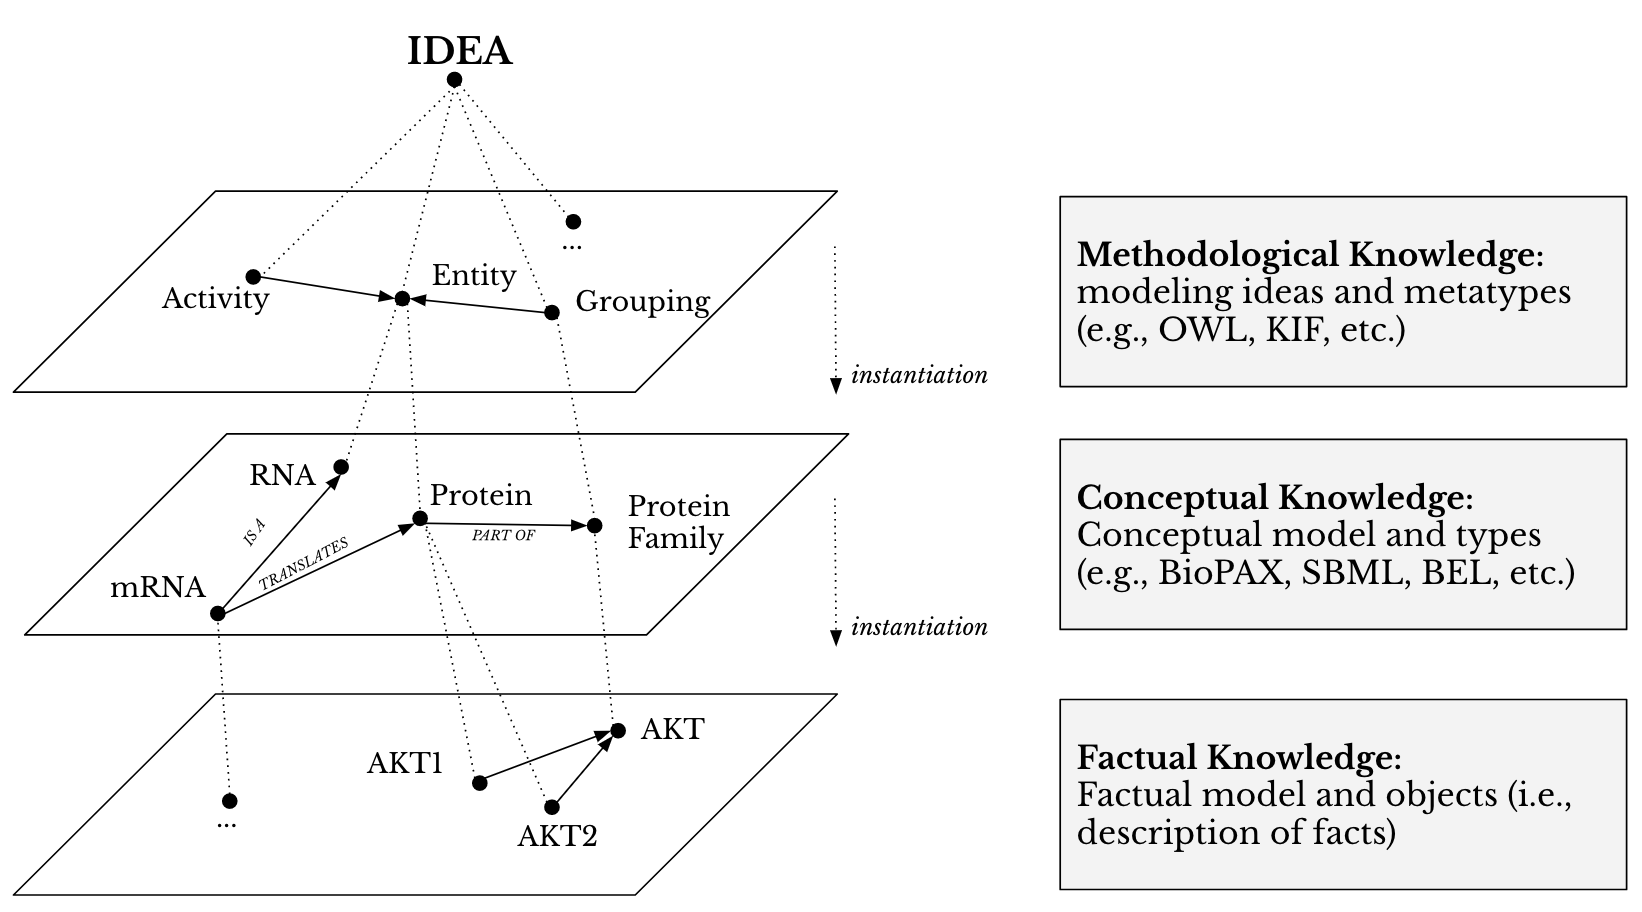
\includegraphics[width=160mm]{images/knowledge_types.png}}
\caption[Levels of Knowledge Abstraction]{The interplay of the three levels of knowledge abstraction in an example from the biological domain.}
\label{Fig:knowledge_types}
\end{figure}
	
\subsection{Resource Description Framework Schema}
    
\ac{RDF} uses triples of subjects, predicates, and objects to represent relations between concepts. Each resource in a triplet is backed by an \ac{IRI}. While its simple format grants it huge expressive power, RDF lacks structure or domain specificity. 

\ac{RDFS} is a set of concepts and predicates appropriate for describing knowledge at the conceptual level. Included are predicates for asserting class hierarchies (\verb|rdfs:subClassOf|), asserting memberships (\verb|rdf:type|), describing the domain and range of predicates (\verb|rdfs:domain|, \verb|rdfs:range|), and representing epistemological concepts such as classes, literals, and other data types \cite{Beckett2014}.

RDF and RDFS are supported by most popular programming languages with packages to serialize and deserialize \ac{RDF} in a variety of formats (e.g., \ac{XML}, N-Triples, turtle, etc.) and reason over \ac{RDFS}.
    
\subsection{Web Ontology Language}

Like \ac{RDFS}, \ac{OWL} consists of the methodological knowledge for modeling domain-specific knowledge. Its most simple form, \ac{OWL} Lite, enables the representation of classes, their properties, relations, and constraints. The most common form, \ac{OWL} \ac{DL}, contains the additional expressive power of descriptive logic over which inferences can be made. The most expressive form, \ac{OWL} Full, removes the remaining restrictions on \ac{OWL} \ac{DL} but paradoxically becomes undecidable and hinders automatic reasoning \cite{Marchetti2008}. The expressive levels of \ac{OWL} are depicted in Figure 2.

\begin{figure}
\captionsetup{format=plain}
\makebox[\textwidth]{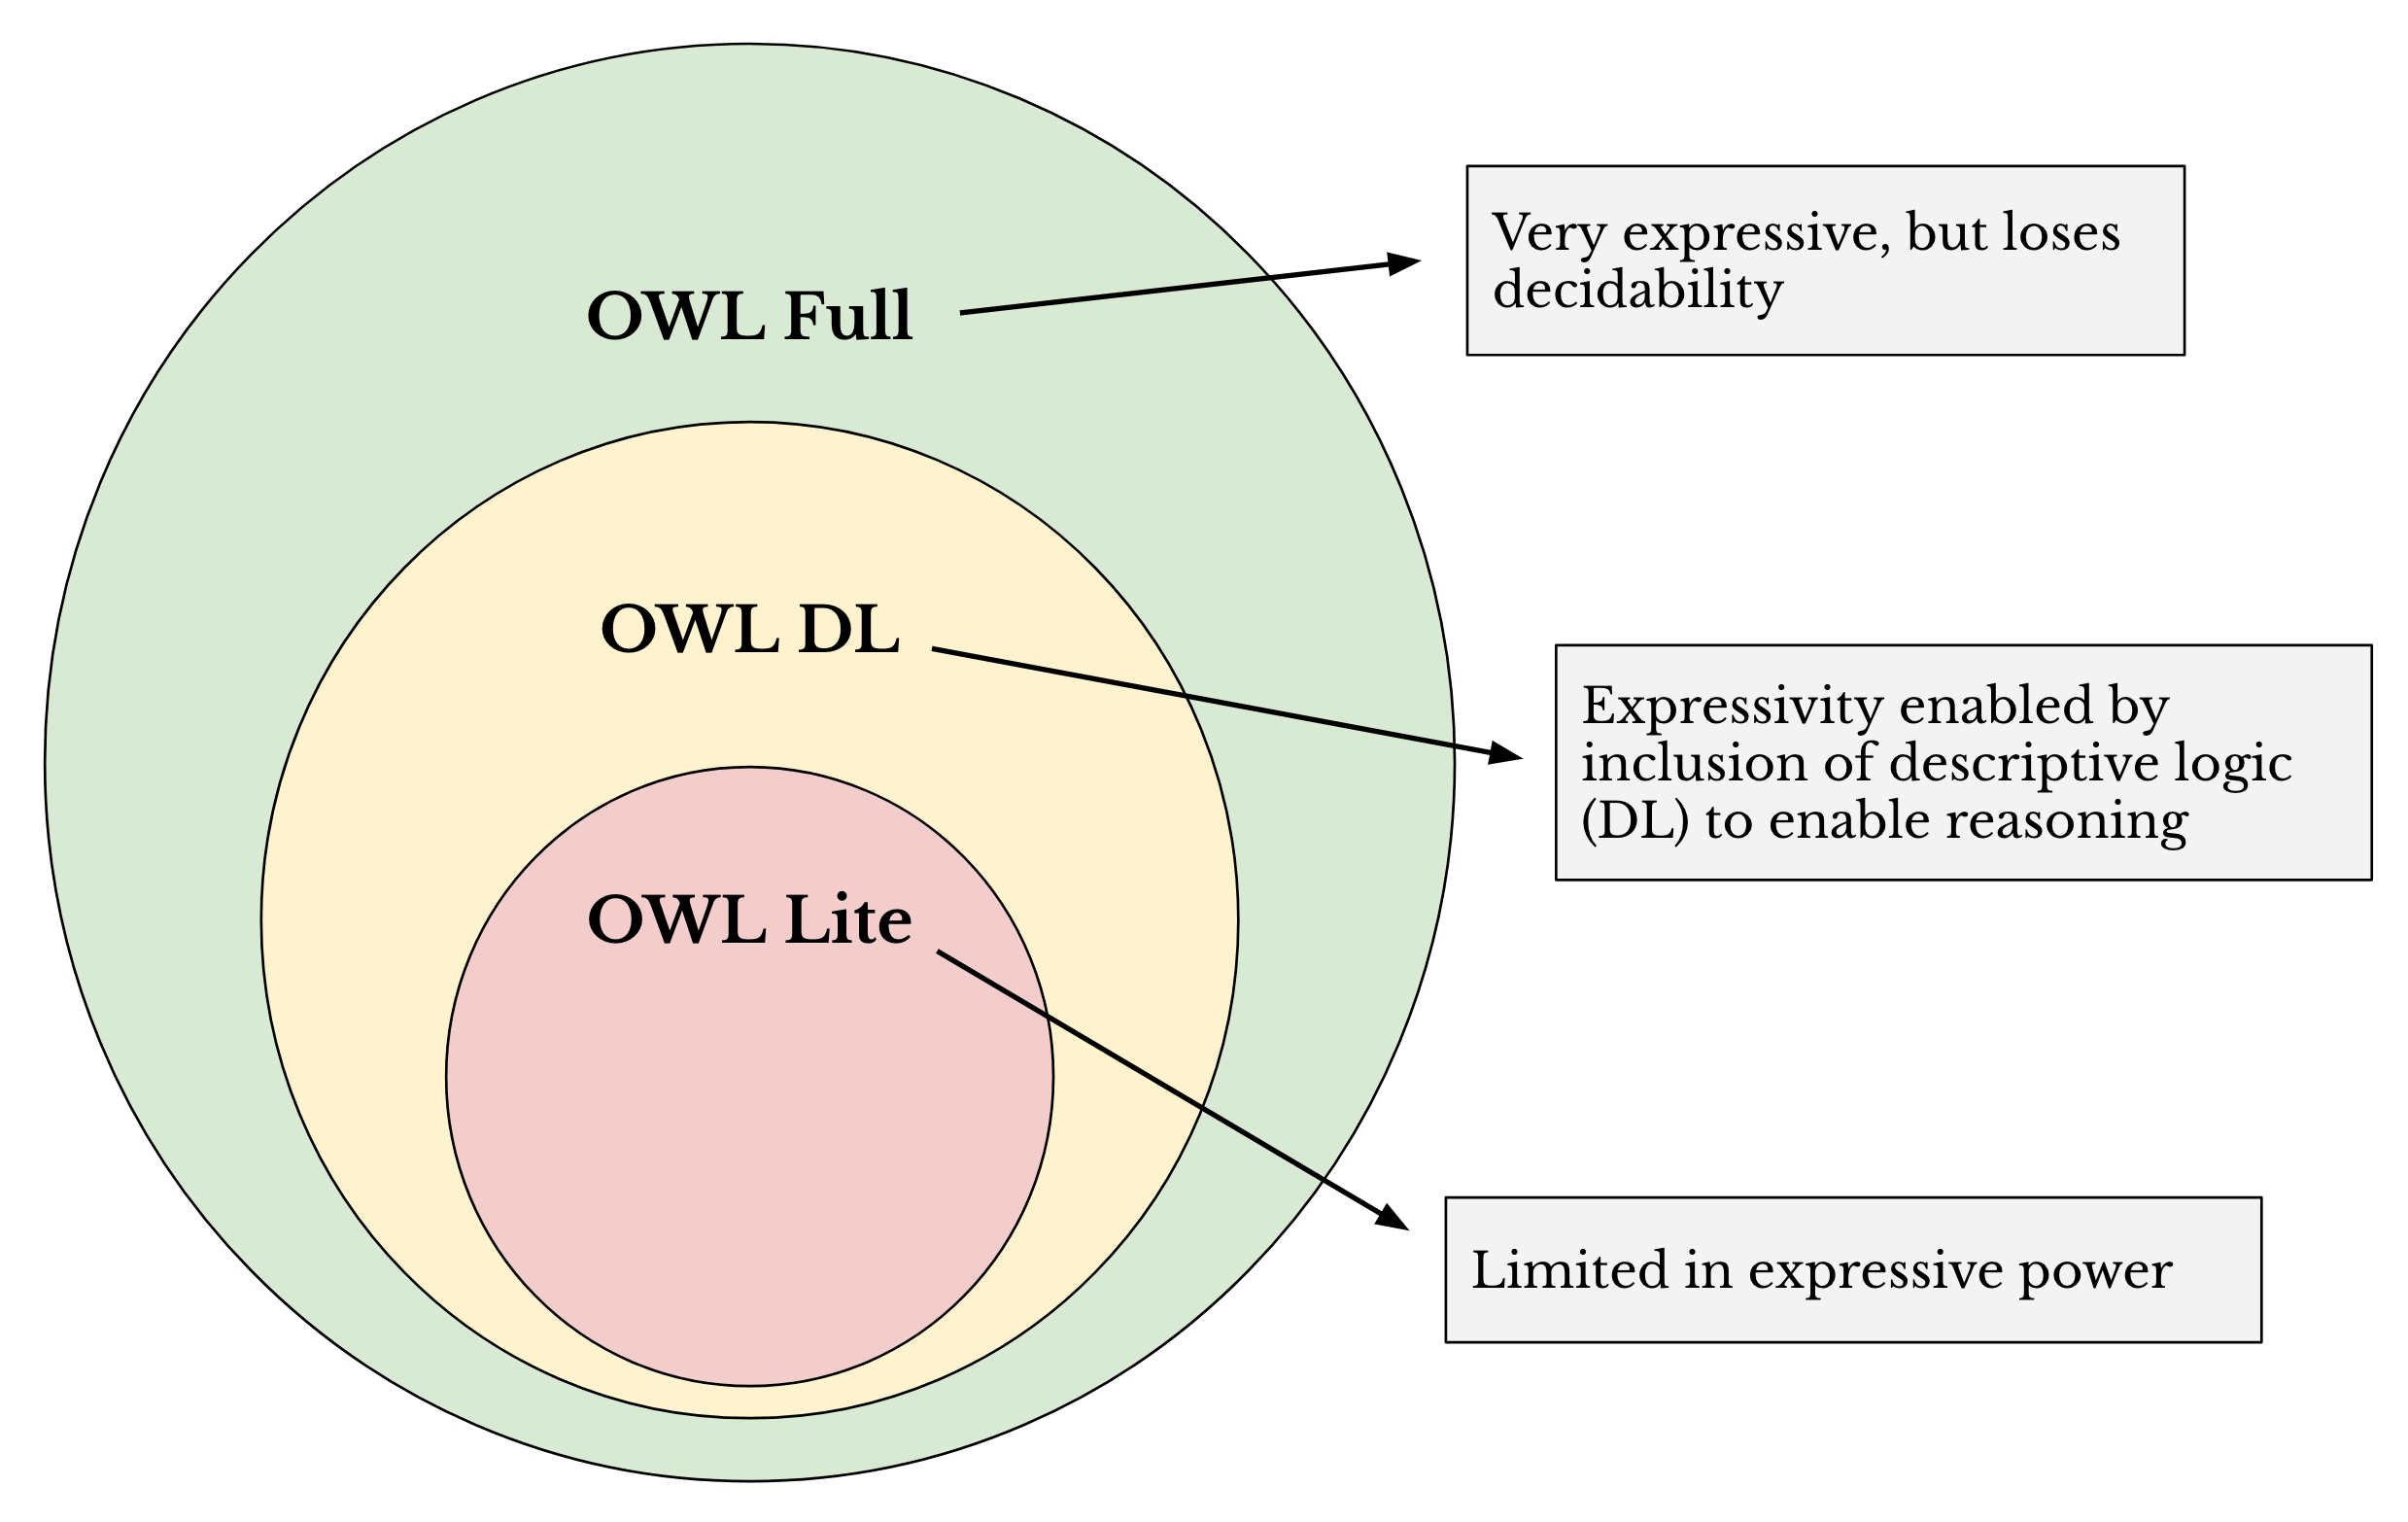
\includegraphics[width=160mm]{images/owl_types.png}}
\caption[Descriptive Levels of OWL]{The expressive levels of OWL ontologies. Adapted from \cite{Marchetti2008}.}
\label{Fig:owl_types}
\end{figure}

\ac{OWL} can be serialized to \ac{RDF}, RDF/XML, OWL/XML, Manchester, and several other formats. As an aside, the community of ontologists has historically used the Java programming language because of the definitive \verb|OWL API| \cite{owlapi} package. Because many bioinformatics tools have been written in the Perl, R, and Python scripting languages, they have been unable to easily make use of the most powerful reasoners available. Development on Python packages (e.g., \verb|OWLReady| \cite{owlready}, \verb|OntoSpy| \cite{ontospy}, \verb|obonet| \cite{obonet}, etc.) is beginning to enable Python programmers to make full use of the abstract concepts introduced in knowledge formalization.

\subsection{Biological Pathways Exchange Language}

\ac{BioPAX} uses \ac{OWL} to define the conceptual knowledge in the domain of biological pathways on the molecular and cellular level. Its ability to collect and index metabolic, signaling, molecular, gene-regulatory, and genetic interaction networks makes it an ideal exchange format for the growing number of pathway databases with varying specificities in regards to target organisms and disease indications \cite{Demir2010}.

This was realized with the aggregation of several pathway and interaction databases (e.g., BindingDB \cite{Gilson2016}, DrugBank \cite{Law2014}, IntAct \cite{Orchard2014}, \ac{KEGG} \cite{Kanehisa2017}, Reactome \cite{Fabregat2016}, WikiPathways \cite{Pico2008}, etc.) to form the Pathway Commons Database \cite{Cerami2011}. Immediately, this database enabled exploration of molecular interactions at the highest granularity. For example, it powers the Enrichment Map Cytoscape Plugin \cite{Merico2010} that was used to support data-driven analysis in identifying medulloblastoma subgraphs based on intratumoral heterogeneity \cite{Cavalli2017}.

\subsection{Systems Biology Markup Language}

\ac{SBML} uses a completely custom formalism defined with \ac{XMLS} to represent the dynamic and quantitative aspects of biochemical reactions, signal transduction, and gene regulatory networks \cite{Hucka2003}. Like \ac{BioPAX}, it provides the conceptual framework necessary to encode knowledge in the biomedical domain. \ac{SBML} also provides the basis for CellDesigner \cite{Funahashi2003}, which has been incredibly successful in allowing biologists without informatics backgrounds to diagram gene regulatory and biochemical networks as well as import them to graphical ordinary differential equation solvers and simulation workflows. 

\subsection{Biological Expression Language}

\ac{BEL} supports the assembly of context-specific qualitative causal and correlative relations between biological entities across multiple scales. Statements are assembled and serialized in \ac{BEL} Script with full provenance information including namespace references, relation provenance (citation and evidence), and relation metadata such as  biological context (i.e. anatomy, cell, disease, etc.) \cite{Slater2014}. The schemata of BEL relations and BEL Scripts are depicted in Figures 3 and 4, respectively.

Data-driven network analyses on \ac{BEL} knowledge assemblies have been successfully performed across a wide variety of clinical applications, including the identification of upstream controllers in hepatocytes \cite{Deehan2012}, mechanistic hypothesis generation for drug response \cite{Laifenfeld2014}, and patient stratification \cite{Laifenfeld2012} by using over-representation analysis techniques developed such as \ac{RCR} \cite{Catlett2013} and pathway topological analytical methods such as \ac{NPA} \cite{Martin2014}. 

\begin{figure}
\captionsetup{format=plain}
\makebox[\textwidth]{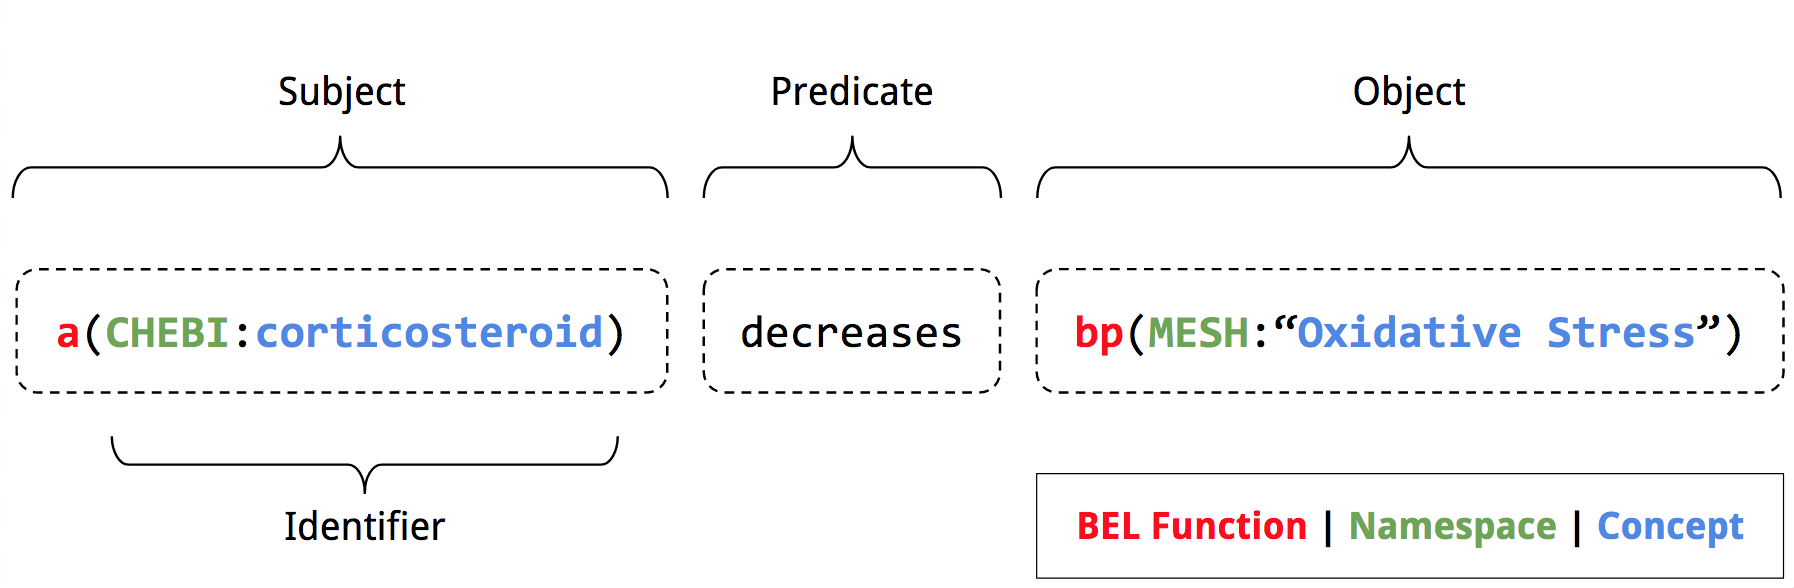
\includegraphics[width=160mm]{images/bel_relation.png}}
\caption[The Schema of a BEL Relation]{A BEL relation is encoded as a triplet containing a subject, a predicate, and an object. The predicate can represents the type of relation while the subject and object can either represent the abundance of molecular entities such as genes, proteins, chemicals, or more abstract concepts such as biochemical reactions, biological processes, and pathologies. Identifiers for these concepts use references to external namespaces (Figure 4B) to qualify their respective names. In this example, \ac{ChEBI} \cite{Hastings2013} is used to qualify chemicals and \ac{MeSH} \cite{ROGERS1963} for biological processes.}
\label{Fig:bel_relation}
\end{figure}

\begin{figure}
\captionsetup{format=plain}
\makebox[\textwidth]{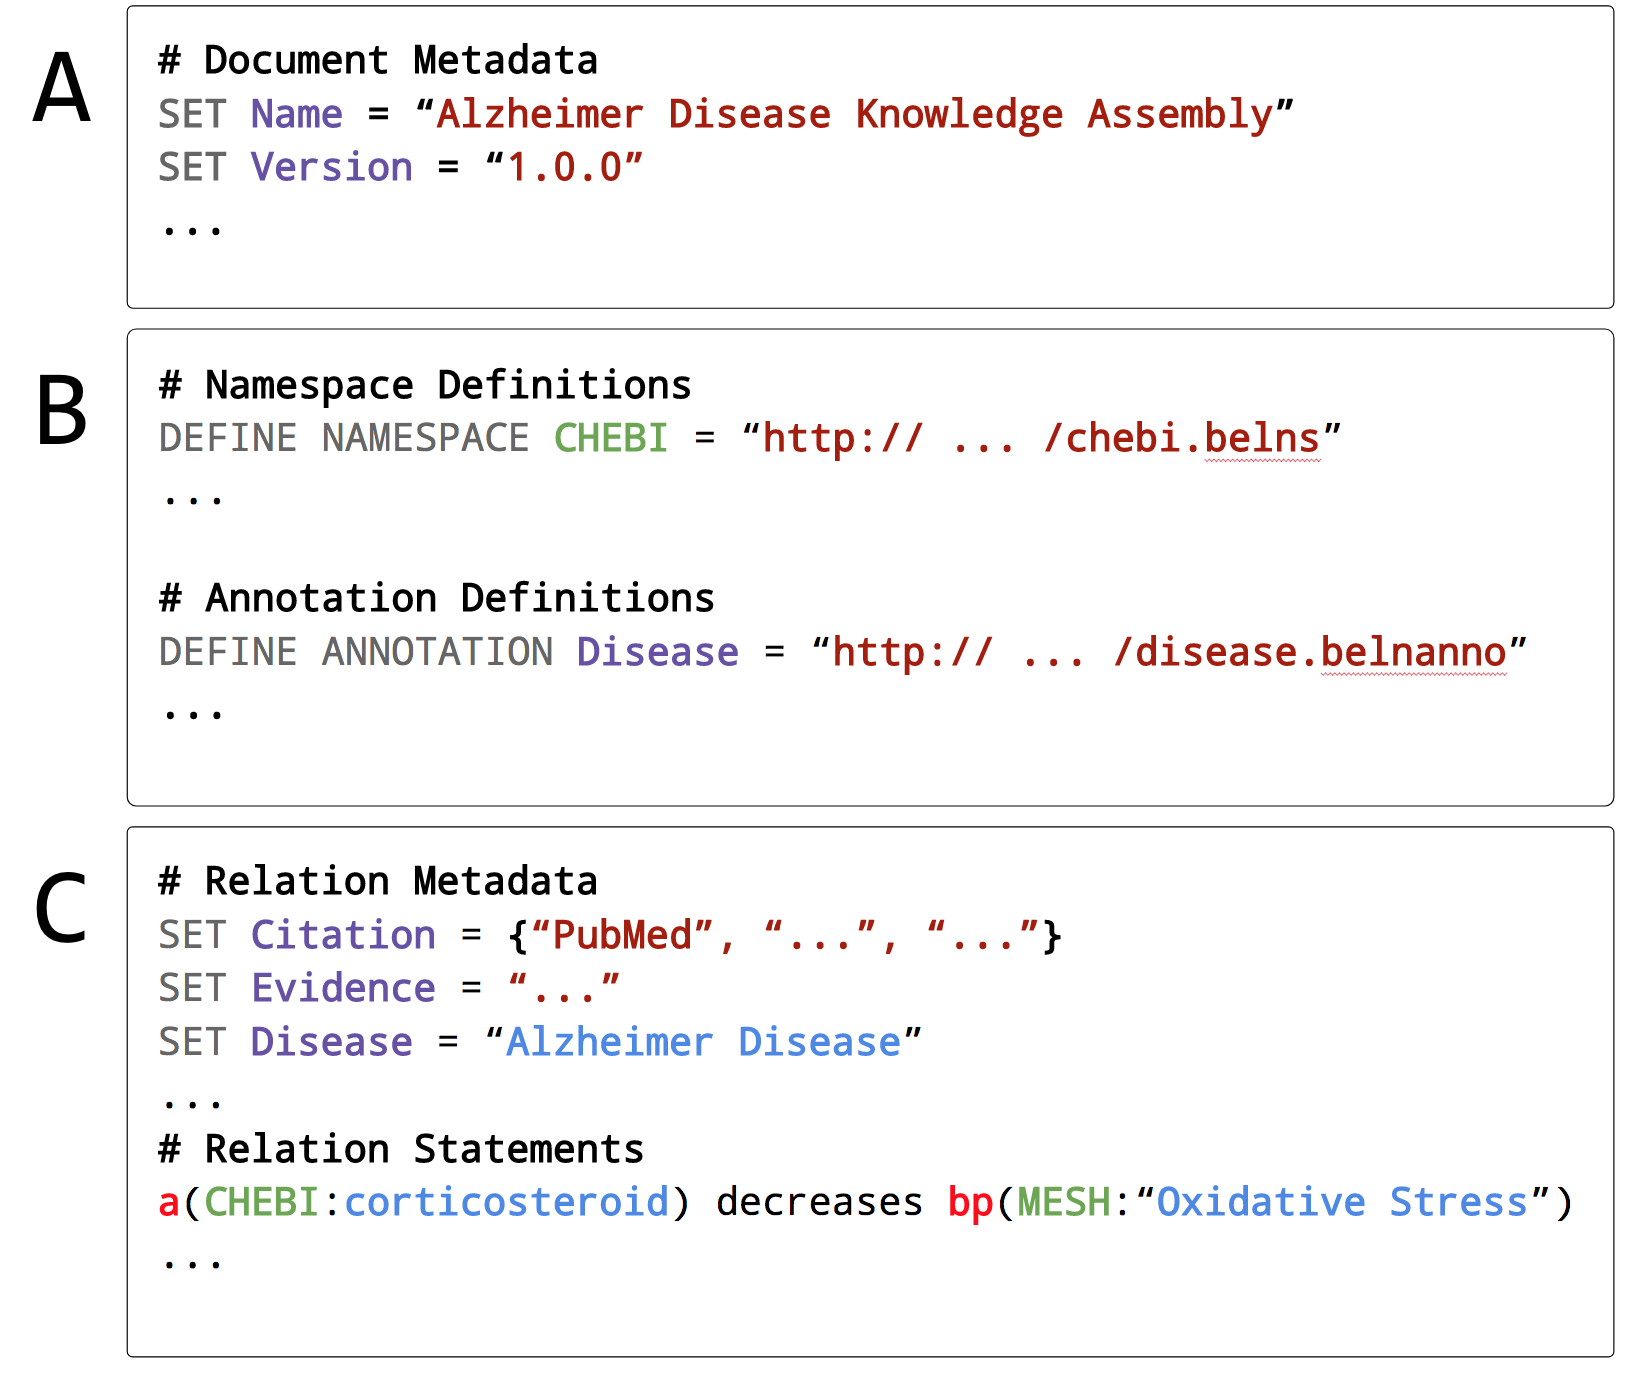
\includegraphics[scale=0.6]{images/bel_script.png}}
\caption[The Schema of a BEL Script]{A BEL Script contains three sections: A) the document metadata section provides provenance information such as the name, version, and author; B) the definitions section provides references to external resources that are used as identifiers and metadata in the relations section; and C) the relations section contains BEL relations and their metadata: minimally including a citation and evidence with the possibility to include additional information such as biological context (e.g. cell, anatomy, disease).}
\label{Fig:bel_script}
\end{figure}

BEL was developed by Selventa, a bioinformatics and computational biology consulting firm, to support knowledge-driven analysis of data. In 2012, they released the \ac{BEL} v1.0 specification as an open standard through the OpenBEL Consortium. However, the inability of BEL to express important concepts in molecular biology (such as genetic variants) prompted the \ac{BEL} v2.0 revision in 2014.

The foray into new disease areas and clinical indications has necessitated the assembly of knowledge on wider scales from the genetic to the phenotypic and population levels. While most modeling languages and data formats for assembling knowledge are insufficient for such a task, BEL possesses the faculty for capturing multi-scale knowledge. 

In the same way \ac{BioPAX} was successful at combining many molecular pathway and interaction database, \ac{BEL} has the potential to serve as a semantic integration platform through which knowledge and data across scales can be integrated and analyzed. \ac{BEL} can be used to reason over the previously untapped sources of chemogenomic and chemical genetic information in the realm of disease-disease, disease-protein, disease-chemical, and chemical-chemical networks.

Modeling interactions across scales is not without its issues. As biological processes, pathologies, and phenotypes represent collections of molecular interactions, they are prone to having excessive associative and correlative relations to other biological entities. This biases typical graph mining algorithms that rely on  graph traversals to visit these types of nodes, and therefore produce less meaningful results. While it is not within the scope of this thesis, there are many solutions for addressing these issues whose complexities vary from simple filtering to empirical traversal rules. or adding extra rules for traversals.

\section{Biological Applications}
\label{biological_applications}

\subsection{NeuroMMSig}

The work in this thesis was carried out in order to support the \ac{IMI} \cite{imisite} project, AETIONOMY \cite{aetionomy}. The goal of this project is to provide a taxonomy of neurodegenerative disease in order to support further development of clinical and computational methods to identify patient subgroups and classify individuals accordingly. 

The first step taken towards this goal was to encode the relevant knowledge surrounding \ac{AD}, \ac{PD}, and Epilepsy in BEL \cite{Kodamullil2015}. Next, a taxonomy of candidate mechanisms was curated in the \ac{NeuroMMSig} Knowledge Base and annotated to these knowledge assemblies \cite{Domingo-Fernandez2017}. These candidate mechanisms contain multiple causal pathways, correlative and associative relations, as well as other related information and are most appropriately named "subgraphs."


\chapter{Motivation \& Outline}
\label{ch:motivation_goal}

\section{Motivation}

The overarching purpose of this master's thesis is to outline the first steps taken towards building a generally reusable, automatic interpretation and hypothesis generation machine.

While many analyses, including those previously referenced, can successfully aid scientists in interpretation of data, each are developed with specific data sets, knowledge assemblies, or application scenarios in mind. Those that were developed using schemata that lacked the generalized multi-scale and multi-modal (schema-free) integration enabled by BEL could have potentially disregarded relevant and important knowledge. 

\section{Outline}

The first section of this thesis describes the PyBEL, the framework built to parse and manipulate BEL Script and resulting knowledge assemblies. The following section describes the development the Bio2BEL data integration framework and the beginning of a cross-scale data integration project similar to Pathway Commons. The final section describes the development of algorithms for analyzing the robustness of knowledge assemblies, preprocessing techniques, and ultimately, proposes a reusable, general, schema-free analytical technique that generates hypotheses with knowledge-driven analyses of data.


\chapter{PyBEL}
\label{ch:pybel}

\section{Survey of Current Technologies}

While there exist several software packages for \ac{BioPAX} and \ac{SBML}, the ecosystem of open-source software for \ac{BEL} is much more limited.

\subsection{OpenBEL Framework}

With its publication of the \ac{BEL} v1.0 specification as an open standard, the OpenBEL Consortium released the OpenBEL Framework \cite{openbelframework} ; a Java framework for parsing BEL v1.0 documents and its companion Cytoscape plugin \cite{openbelframeworkcytoscapeplugins} for network visualizations.

\subsection{bel.rb}
Ongoing development slowed \cite{openbelframeworkgraphs} as the focus of OpenBEL development shifted towards \verb|bel.rb| \cite{belrb}; a Ruby tool for parsing and transforming BEL v1.0 Script to \ac{RDF}. Additionally, there is only limited community support through GitHub and the proposed channel on Gitter.

Neither of the previously mentioned softwares provide explicitly documented support for this revision; and the aging codebase of the OpenBEL Framework and the generally low usage of Ruby in the bioinformatics community provide little incentive for updates. 

\section{Motivation}

There is an unmet need for publicly available, easily installable, stable, facile software that parses modern BEL and provides programmatic access to a data container that enables the resulting network to be extended, queried, manipulated, analyzed, and visualized. Furthermore, a converter between common data formats is needed to enable re-usability and interoperability between general and BEL-specific software for network analysis and visualization. This chapter presents PyBEL, a Python language software package designed to fulfill each of these needs.

\section{Software Architecture}

Development of the PyBEL software package adheres to a component-based software architecture. The schematic view in Figure 5 illustrates how data flows between components. components interact to build an integrated environment for working with networks encoded in BEL Script. 

\begin{figure}
\captionsetup{format=plain}
\makebox[\textwidth]{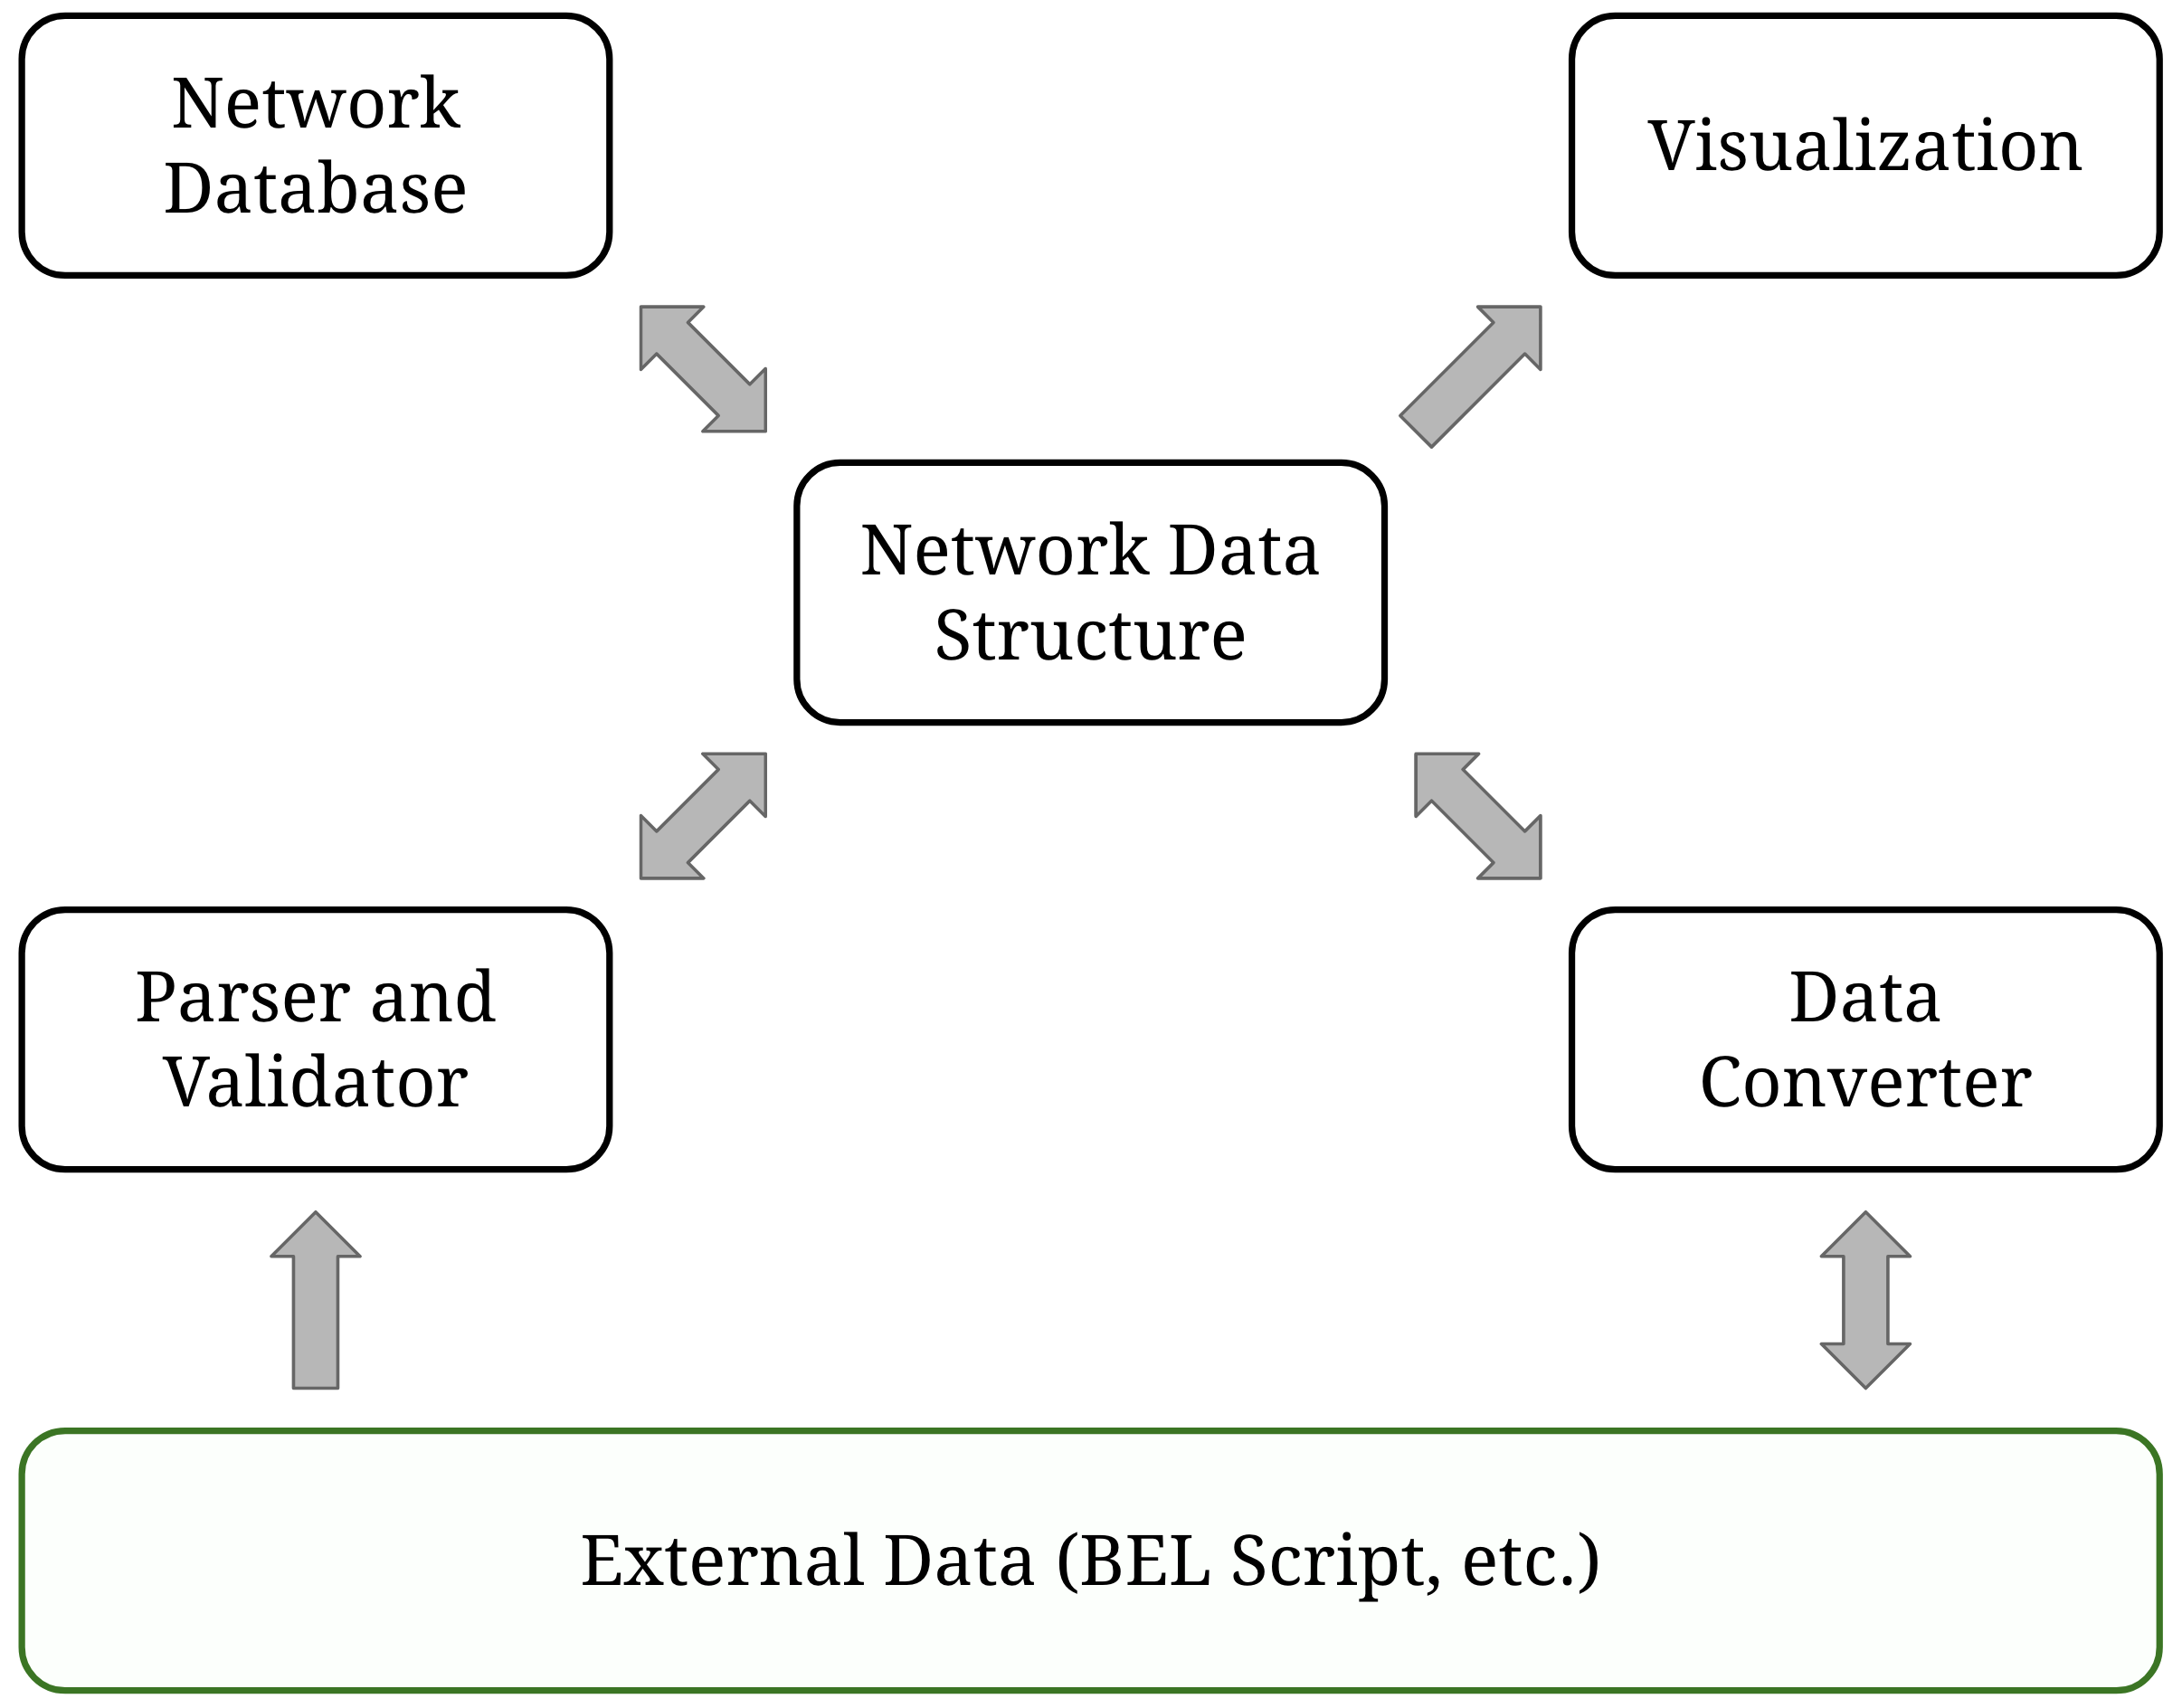
\includegraphics[width=120mm]{images/pybel_components.png}}
\caption[The PyBEL Software Architecture]{The PyBEL software package consists of five main parts: (1) the data container, (2) the parser and validator, (3) the network database, (4) the data converter, and (5) visualization. Arrows represent the direction of the flow of data between components. Together, these components provide a framework for developing tools for exploration and analytics.}
\label{Fig:pybel_components}
\end{figure}

\subsection{Network Data Container}
While a graph refers to an abstraction for a set of objects (i.e. nodes) and their relations (i.e. edges), its instantiation in a real-world application is often called a network. PyBEL implements a directed multigraph (i.e. a graph whose edges have directionality and any given pair of nodes may have multiple edges) that maps the biological entities and concepts in the subjects and objects of \ac{BEL} relations to nodes in a network and their relations, with corresponding metadata, to edges. It extends the MultiDiGraph class from NetworkX, a Python package for manipulation of networks \cite{Hagberg2008}, to enable users direct access to their suite of network algorithms and provide additional tools to develop them into biologically meaningful analyses. While no-SQL database systems like Neo4J \cite{neo4j} are also able to store and make increasingly complicated queries over networks, they inherently lack the extensibility of data structures native to programming languages like Python that can be extended and directly manipulated.

Additional information can be annotated on each of the node, edge, and graph levels. This can allow of the integration of tabular information (i.e. differential gene expression on nodes or $IC_{50}$ values for edges representing inhibition experiments of chemicals on enzymes). Network-level annotations allows for storage of all relevant provenance information related to curation and namespace definitions in order to enable semantic data integration with other network and tabular data sources. 

\subsection{Parsing and Validation}

The parser combines components for performing tokenization, lexical analysis, parsing, and validation on each of the three sections of BEL Script. Each was implemented using the internal domain-specific language provided by the PyParsing \cite{pyparsing} Python package because of its exceptional speed, ease of writing compared to regular expressions, and ability to register callbacks for different language features. One callback annotates the entries in the document metadata section to a network instance while another downloads and stores the resources referenced in the definitions section. The relations section has two main callbacks; one to maintain a list of current annotations from SET statements and another to parse BEL relations (Figure 4C-D) and populate a network instance with the corresponding nodes, edges, and their metadata from the current internal state.  

While relations' syntax is implicitly validated by the implementation of BEL in PyParsing, the semantics of their subjects' and objects' identifiers are validated with the references stored earlier. Finally, feedback is provided to users with thorough error analyses to support thoughtful re-curation, which could lead to more robust knowledge assemblies and enable more reproducible science.

\subsection{Network and Edge Store}

PyBEL uses a relational database to cache external namespaces and pre-parsed networks to improve the speed of validation and access to data. While relational databases are not generally appropriate for applying network algorithms, they do provide indexing functionality that enables complicated queries and filters over the nodes, edges, and metadata of increasingly large collections of networks. For example, this could enable the identification of intersections and potential cross-talk in different disease-specific networks. SQLAlchemy \cite{sqlalchemy}, a popular object-relational mapper, was used to maintain the database schema, transport the results of queries to PyBEL, and enable integration of external relational databases. Additionally, SQLAlchemy supports both fully-featured relational database management systems as well as SQLite \cite{sqlite} for a zero-configuration option. 

\subsection{Data Converter}

Lossless conversion protocols were implemented for common file formats including Node-Link \ac{JSON}, \ac{JGIF}, CX, and Python Pickle as well as for multiple common database formats including \ac{SQL}, Neo4J, and the \ac{NDEx} (Table 1). Additional lossy exporters were provided to \ac{CSV}, \ac{SIF}, Excel, \ac{XGMML}, and \ac{GSEA} and \ac{GRP} to facilitate usage in other programs (Table 2). Notably, implementing a RDF converter was deferred until improvements are made to the existing BEL to RDF mapping and its documentation \cite{openbelrdf}.

\begin{table}
\centering
\caption[PyBEL Interconversion Formats]{Multiple lossless converters are provided to common file formats and databases. Full descriptions of the programmatic API can be found at http://pybel.readthedocs.io/en/latest/io.html}
\label{tab:conversion}
\def\arraystretch{1.5}
\begin{tabular}{p{2cm} p{12cm}}
Format & Usage \\
\hline
BEL Script & Output to BEL scripts results in upgrade of statements from BEL v1.0 and a standardized formatting. \\
Binary & Using Python’s pickle module, pre-parsed BEL Script can be stored as binary data for fast loading, storage in databases, and transfer via network protocols. \\
Node-Link & Node-Link \cite{nodelink} is the standard \ac{JSON} format for many web-based network visualization tools, including D3.js \cite{d3js}. Output is facilitated by standard code provided by NetworkX. \\
JGIF & \ac{JGIF} \cite{jsongraphformat} is defined by a schema that is nearly a proper subset of the Node Link format. Conversion with this format provides compatibility with other software and repositories, such as the Causal Biological Network Database \cite{Talikka2015}. \\
CX & CX \cite{cxmodel} is an aspect-oriented network interchange format encoded in JSON with a format inspired by the JSON-LD \cite{jsonld} encoding of RDF. It is primarily used by the \ac{NDEx} and more recent versions of Cytoscape. \\
NDEx & PyBEL contains wraps the \ac{NDEx} Python client \cite{ndexpython} for seamless upload/download to the \ac{NDEx} in the CX format. \\
SQL & SQLAlchemy is used to make abstract queries over the nodes and edges of a collection of networks. \\
Neo4J & Neo4J  is a graph database that enables complex graph queries with the Cypher querying language.
\end{tabular}
\end{table}

\begin{table}
\centering
\caption[PyBEL Export Formats]{Exporters to lossy and irretrievable formats are provided to promote usability in other programs.}
\label{tab:lossy_exporters}
\def\arraystretch{1.5}
\begin{tabular}{p{2cm} p{12cm}}
Format              & Usage \\
\hline
CSV, SIF, and Excel & \ac{CSV}, \ac{SIF}, and Excel all consist of an edge list with interaction types that are suited for viewing in Excel or Cytoscape.                                                                                              \\
XGMML               & \ac{XGMML} \cite{xgmml} supersedes \ac{GML} by adding support for both node and edge annotations. Its name derives from its encoding in \ac{XML}. It can be directly imported to Cytoscape for viewing. \\
HTML                & Interactive visualizations can be produced using JSON export and D3.js. They can be embedded directly in Jupyter Notebook.                                                                                                                                                  \\
GSEA                & This export option outputs a list of genes in the \ac{GRP} format for use with the Broad Institute’s \ac{GSEA} platform \cite{Subramanian2005}.
\end{tabular}
\end{table}


\subsection{Visualization}

Networks can be exported to \ac{CSV}, \ac{SIF}, \ac{XGMML}, or CX for visualization in Cytoscape \cite{Franz2015} or uploaded to \ac{NDEx} \cite{Pratt2015} to take advantage of its viewer and simple query interface. Alternatively, PyBEL provides an interactive network explorer and visualizer that is tailored to \ac{BEL} networks (appropriate node coloring, metadata pop-ups, etc.) that can be directly embedded as \ac{HTML} in email, Jupyter Notebook \cite{Kluyver2016}, or a web application. For example, it has already been used to produce visualizations in the NeuroMMSig web server \cite{Domingo-Fernandez2017}. Figures 6-8 present the Alzheimer’s Disease Knowledge Assembly Wnt Signaling Subgraph from \ac{NeuroMMSig} in three different visualizations.

\begin{figure}
\captionsetup{format=plain}
\makebox[\textwidth]{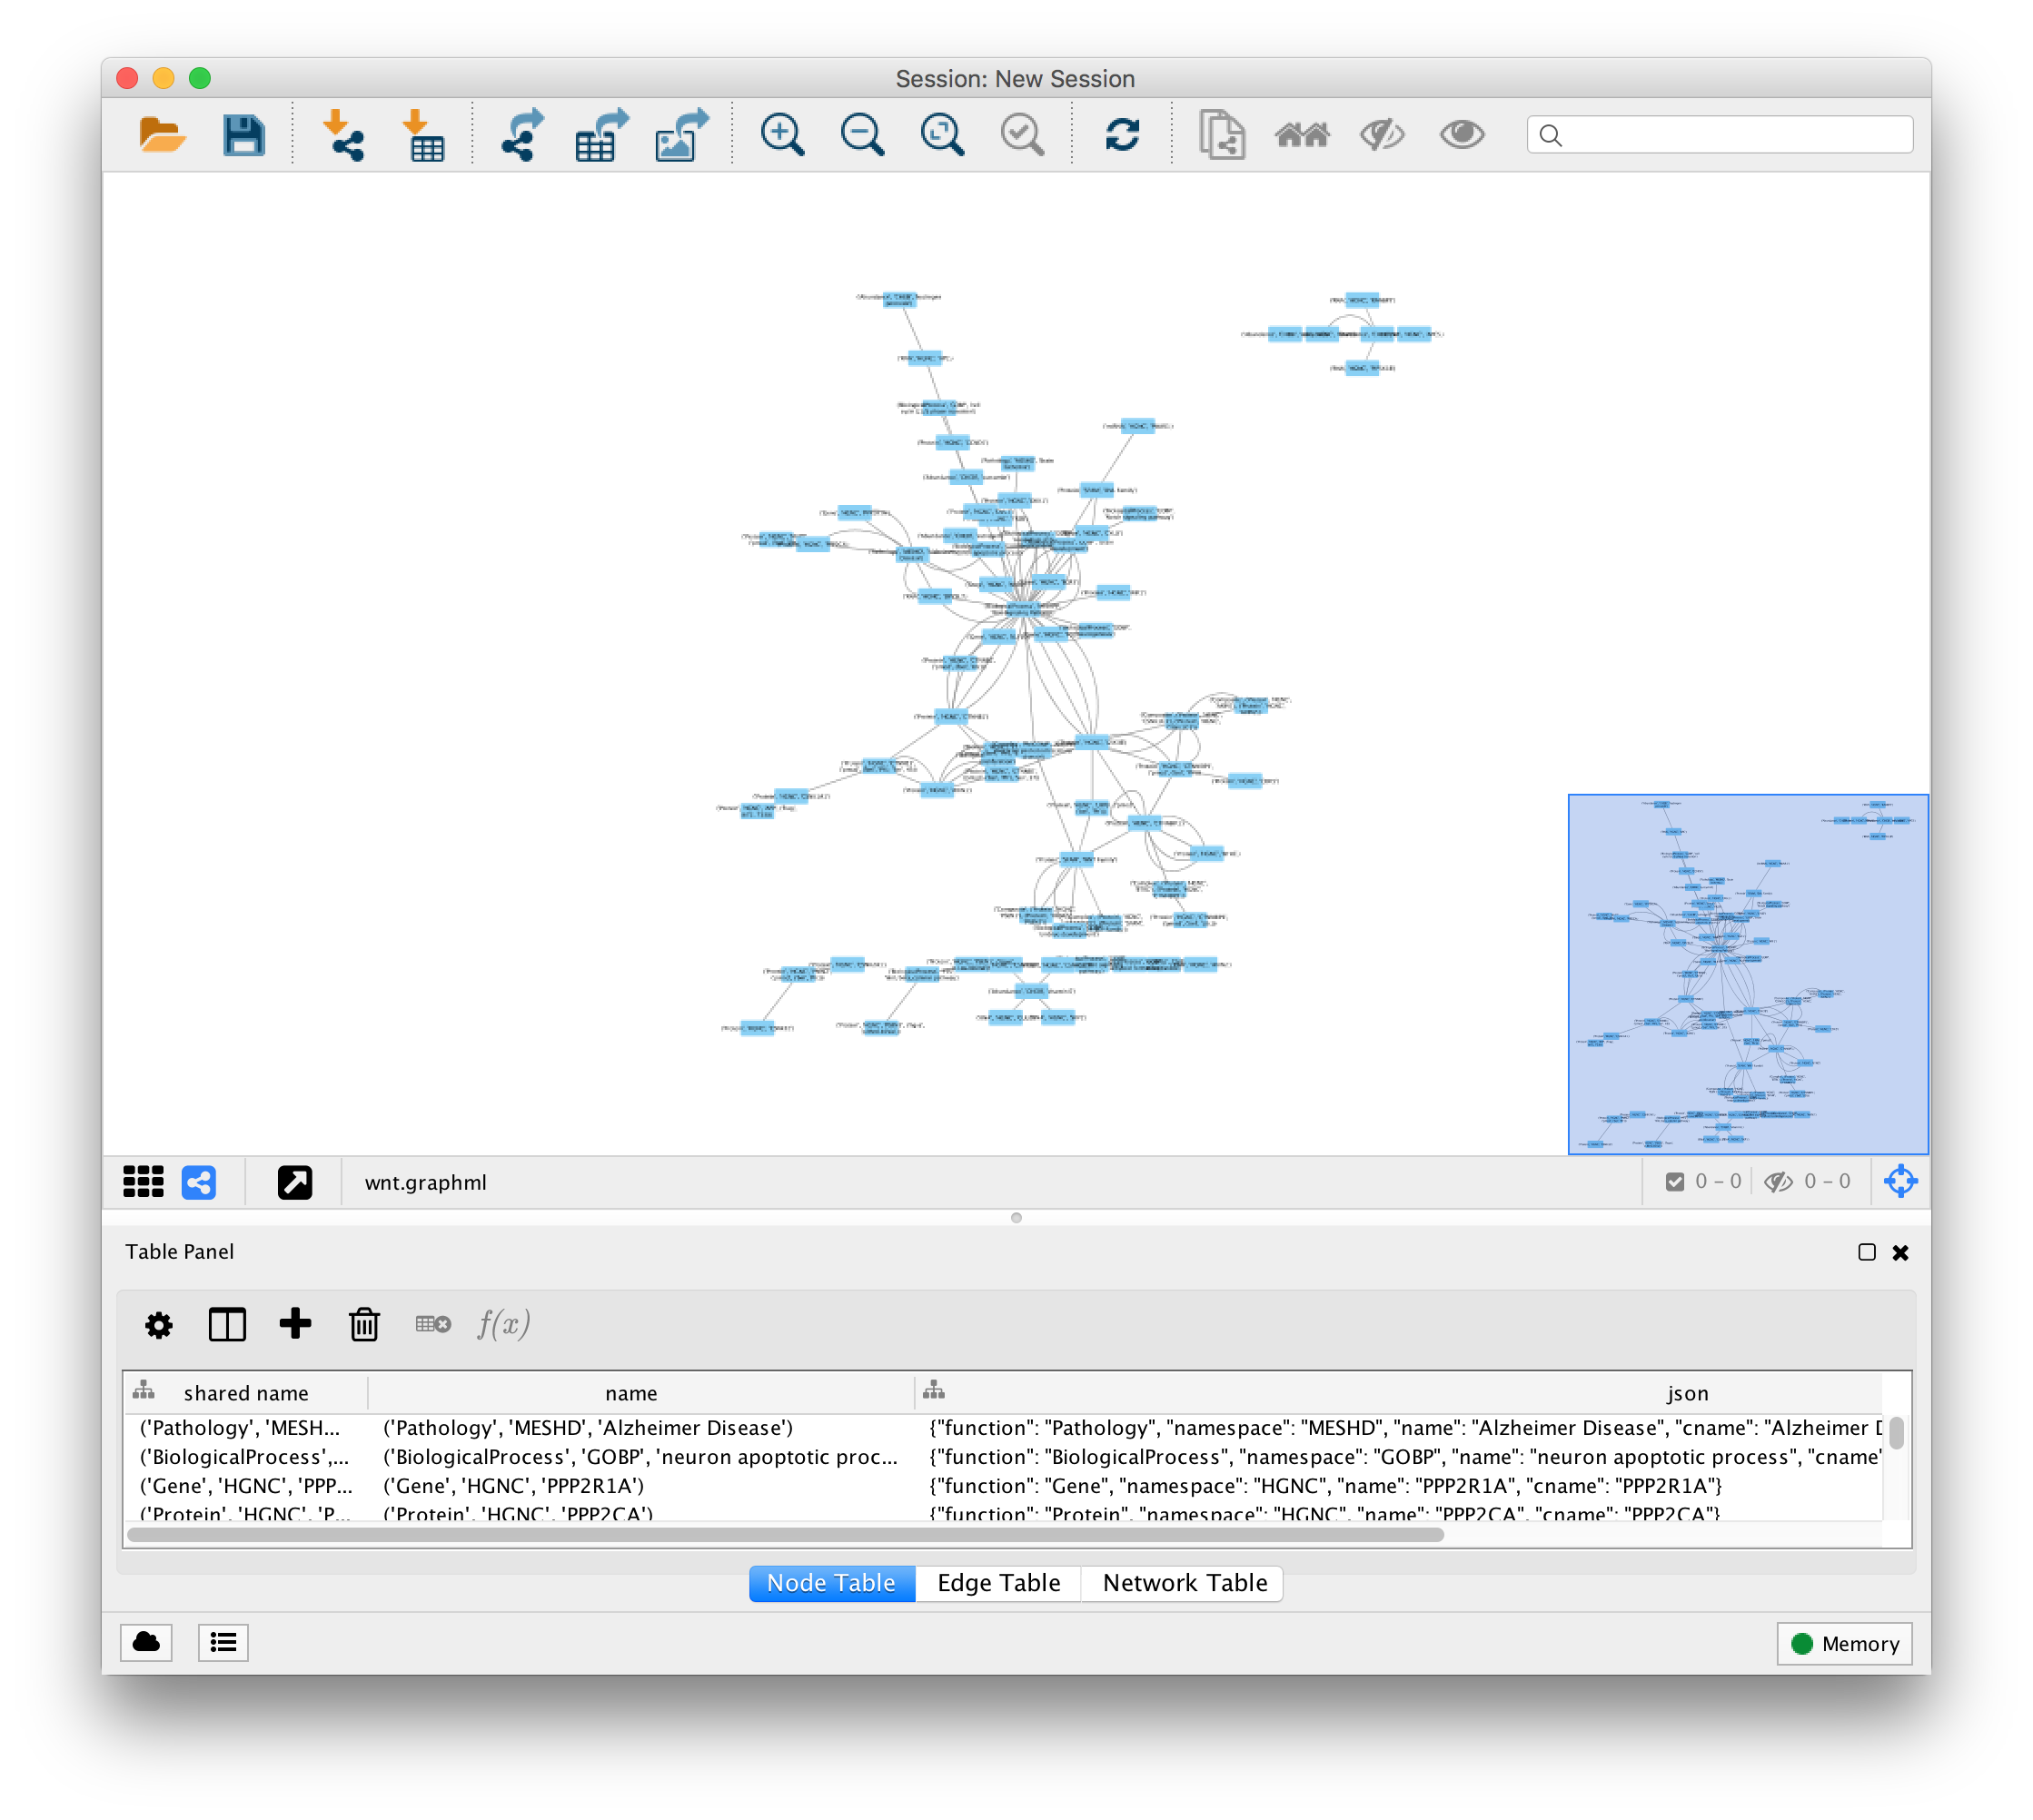
\includegraphics[width=160mm]{images/wnt_cytoscape.png}}
\caption[PyBEL Visualization of Wnt Signaling in Cytoscape]{Visualization of the Wnt Signaling Subgraph from the \ac{NeuroMMSig} Alzheimer’s Disease Knowledge Assembly with Cytoscape provides extensive styling and rudimentary access to the node and edge properties stored in PyBEL. Cytoscape also provides some network analytics functions.}
\label{Fig:wnt_cytoscape}
\end{figure}

\begin{figure}
\captionsetup{format=plain}
\makebox[\textwidth]{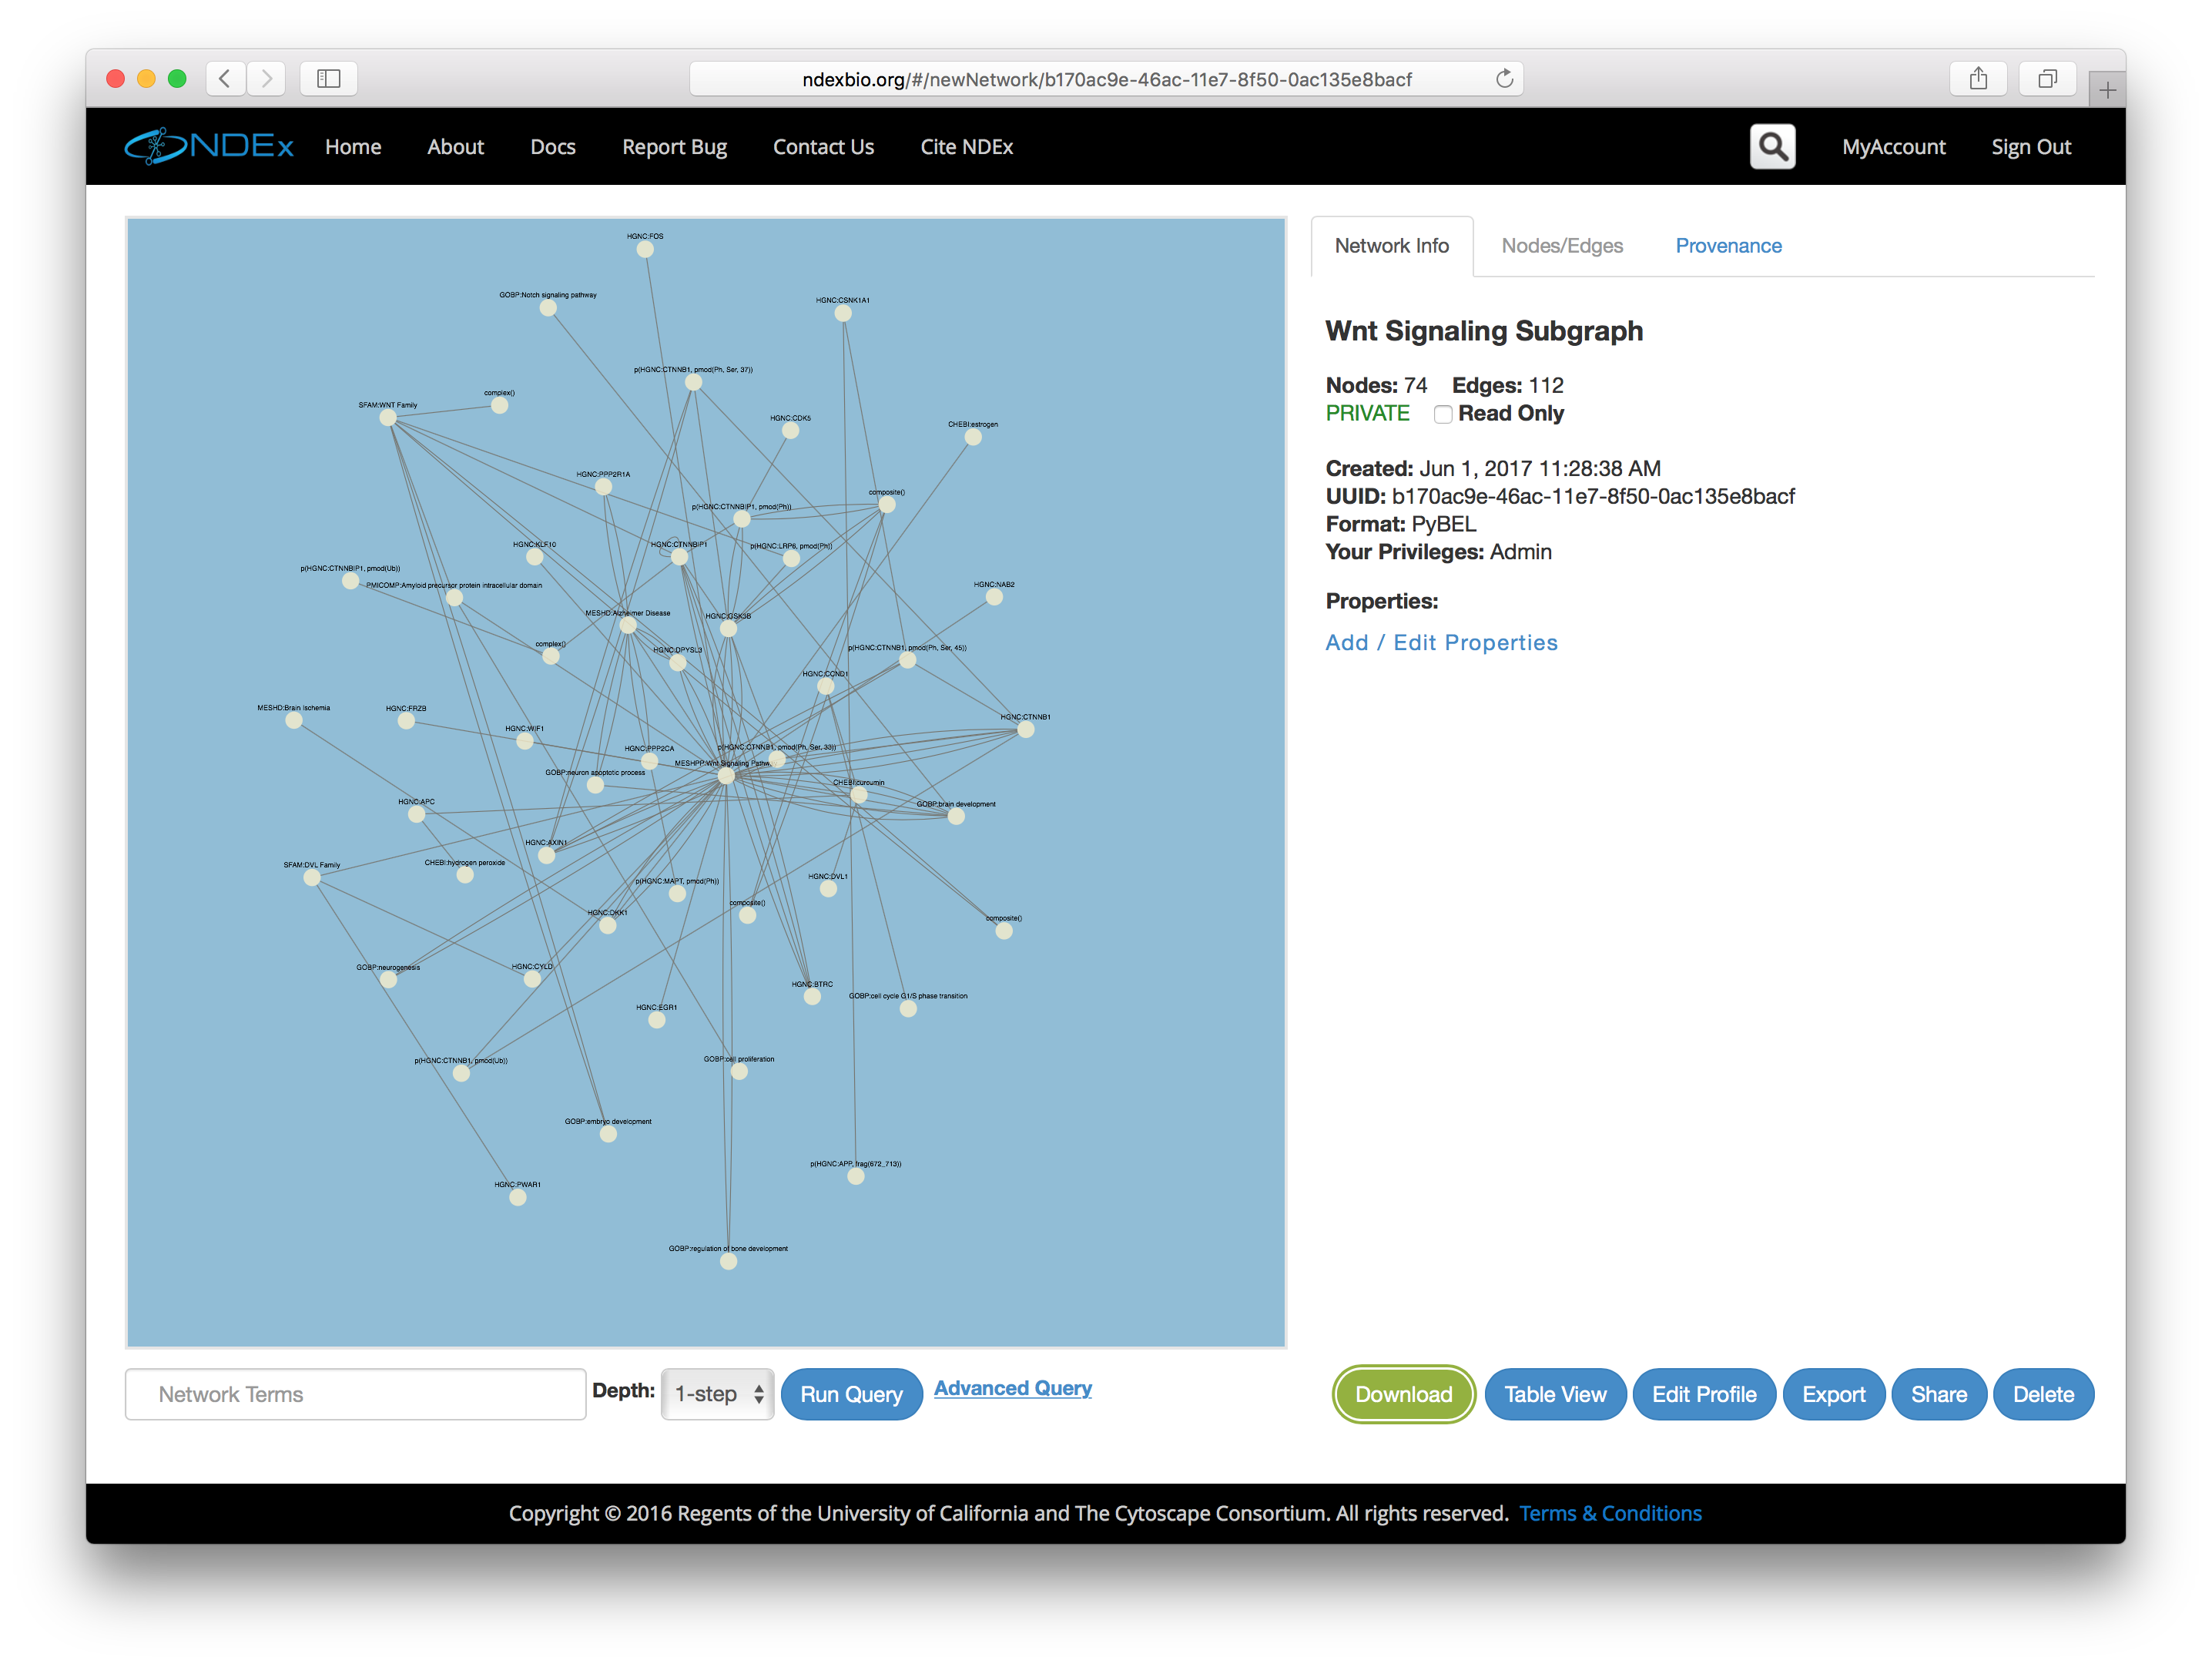
\includegraphics[width=160mm]{images/wnt_ndex.png}}
\caption[PyBEL Visualization of Wnt Signaling in NDEx]{Visualization of the Wnt Signaling Subgraph from the \ac{NeuroMMSig} Alzheimer’s Disease Knowledge Assembly with \ac{NDEx} allows users to easily share their networks.}
\label{Fig:wnt_ndex}
\end{figure}

\begin{figure}
\captionsetup{format=plain}
\makebox[\textwidth]{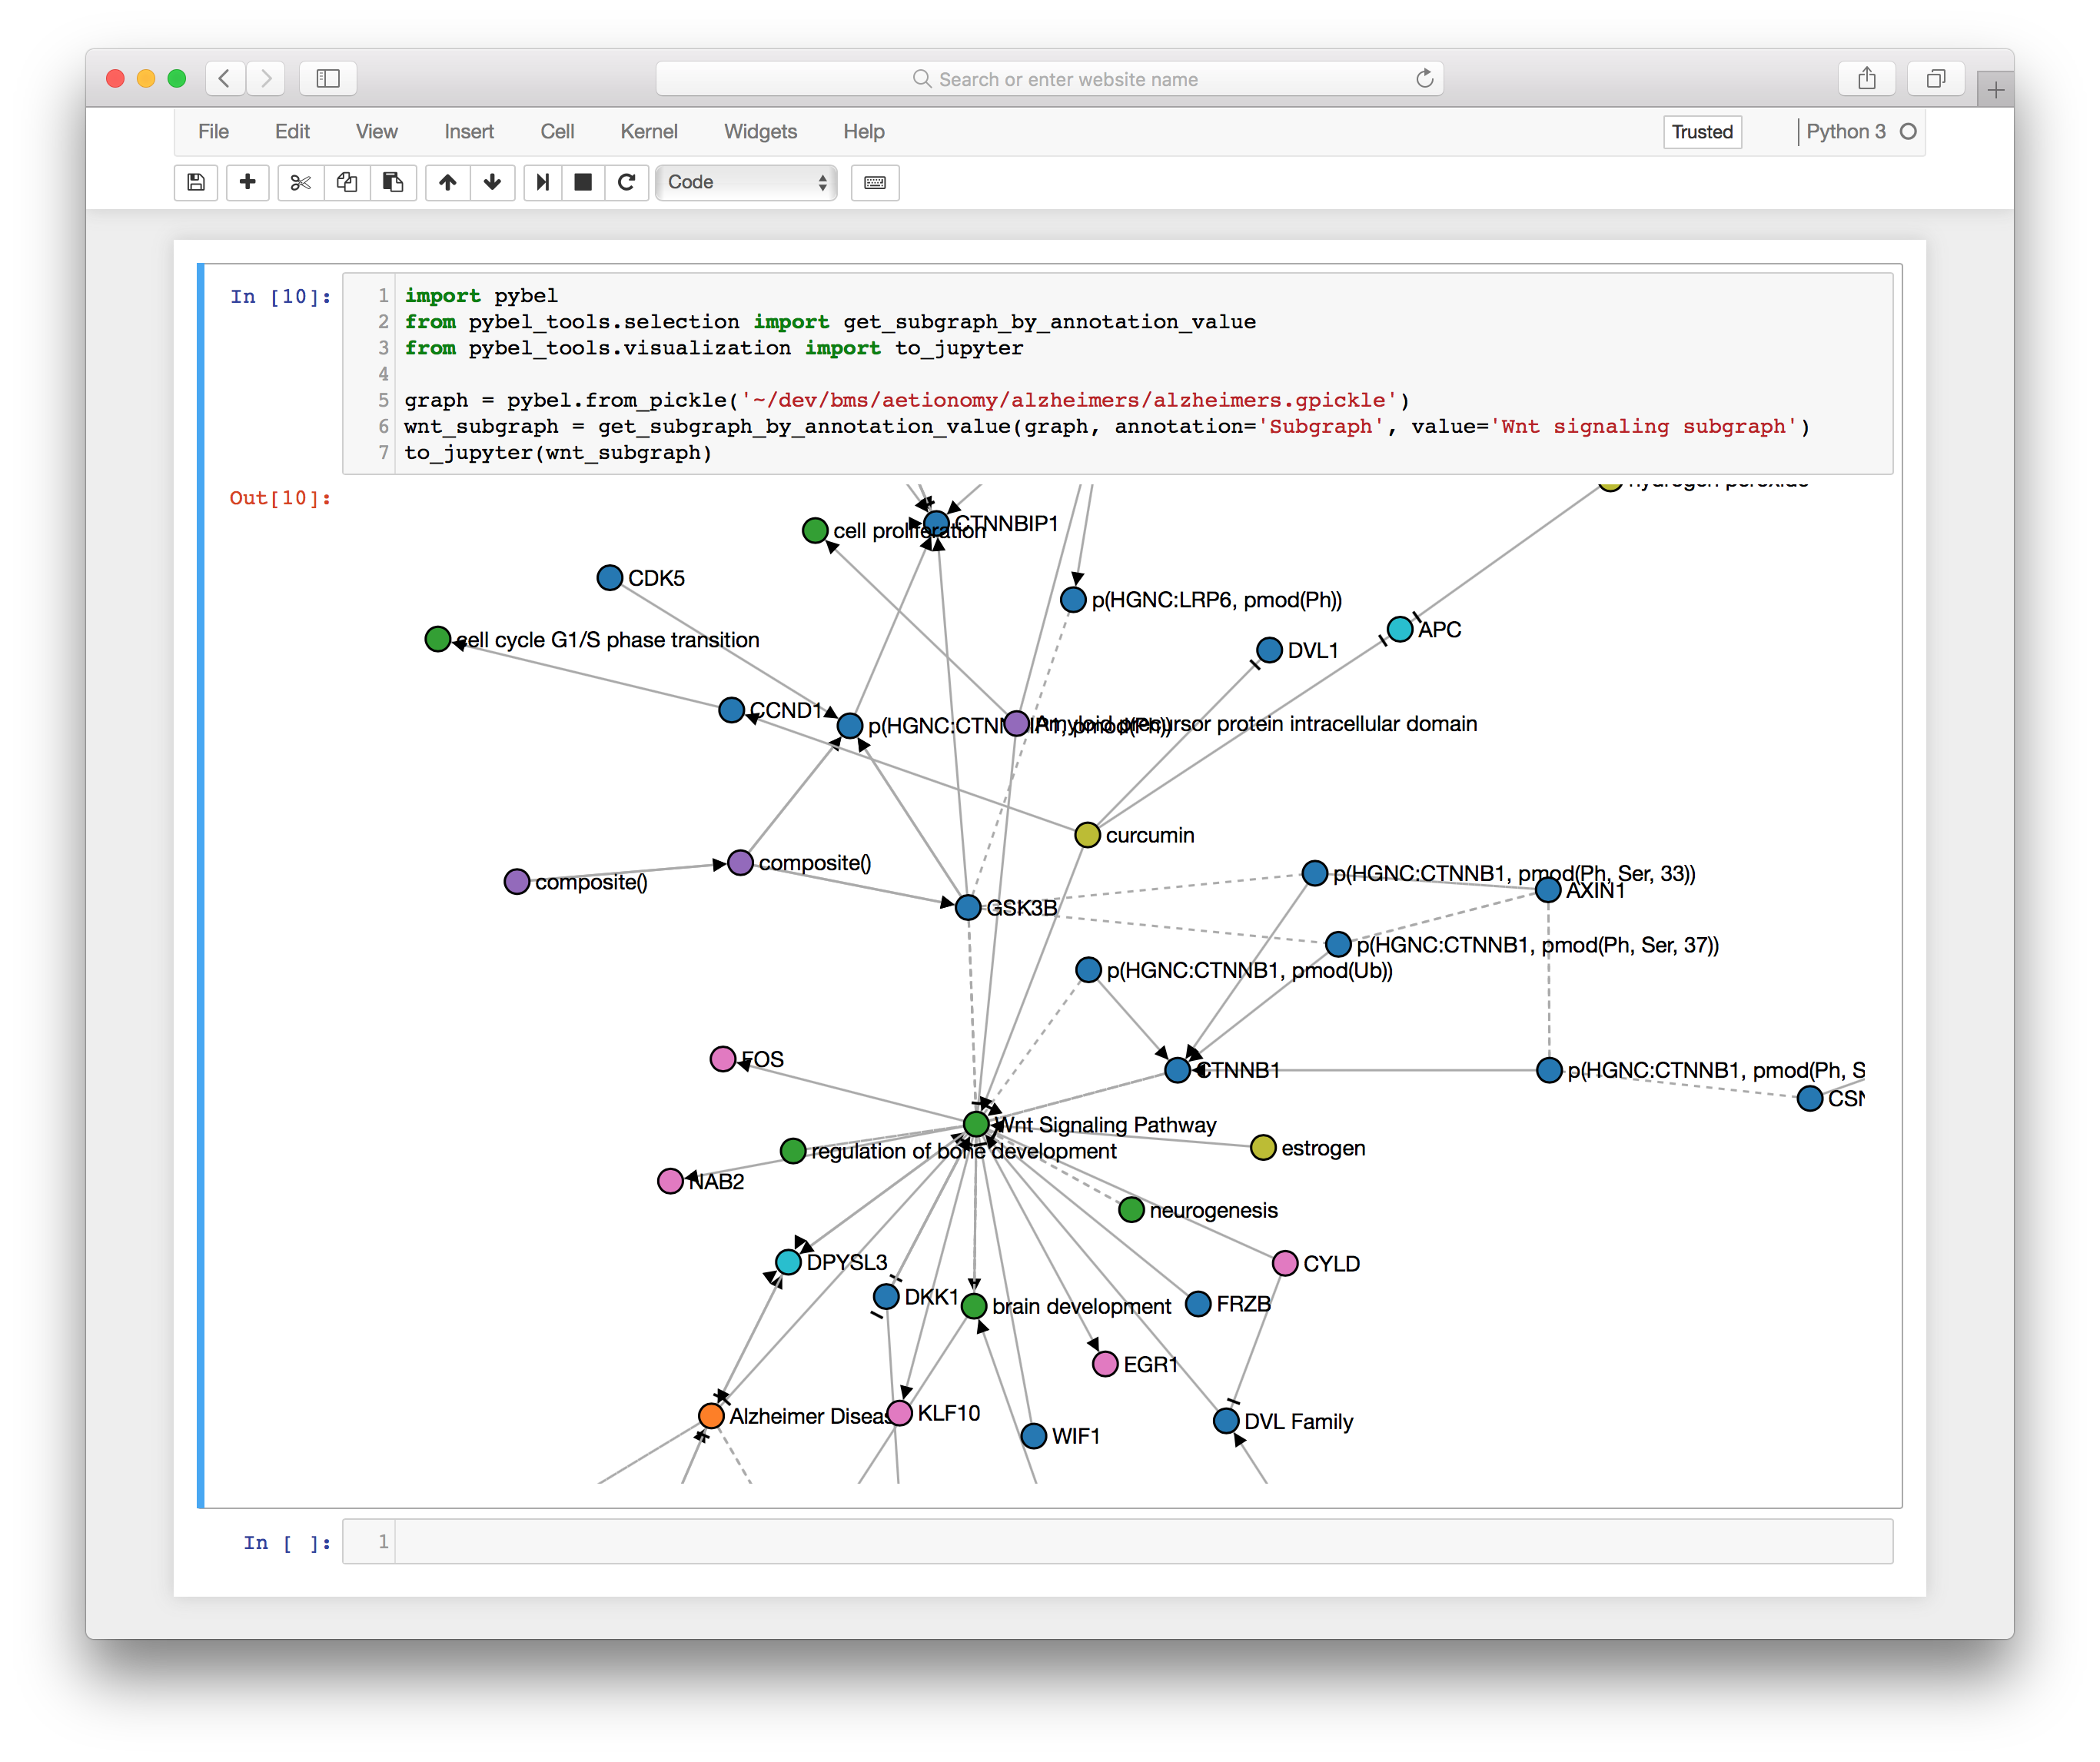
\includegraphics[width=160mm]{images/wnt_jupyter.png}}
\caption[PyBEL Visualization of Wnt Signaling in Jupyter Notebook]{Visualization of the Wnt Signaling Subgraph from the NeuroMMSig Alzheimer’s Disease Knowledge Assembly with Jupyter Notebook allows for embedding within scientific workflows.}
\label{Fig:wnt_jupyter}
\end{figure}

The visualization system from PyBEL has been built in a modular way so it can be integrated in other applications. The underlying Javascript and \ac{HTML} are written with the Jinja templating language \cite{jinja} and exposed via Python functions that can be integrated in Python code or exposed through a RESTful \ac{API}. There is ongoing work to enable users to easily visually explore the results of the \ac{BELIEF} \cite{Madan2016} and \ac{INDRA} \cite{indra} text mining pipelines. Other projects, such as the development of a web service to display and explore a knowledge base assembled for an ongoing project related to \ac{PTSD} are also currently using the PyBEL visualization to embed specific knowledge assemblies with other clinical and molecular data. Figures 9-11 present the PyBEL visualization embedded in other applications that are already in the prototype or release stage of development.

\begin{figure}
\captionsetup{format=plain}
\makebox[\textwidth]{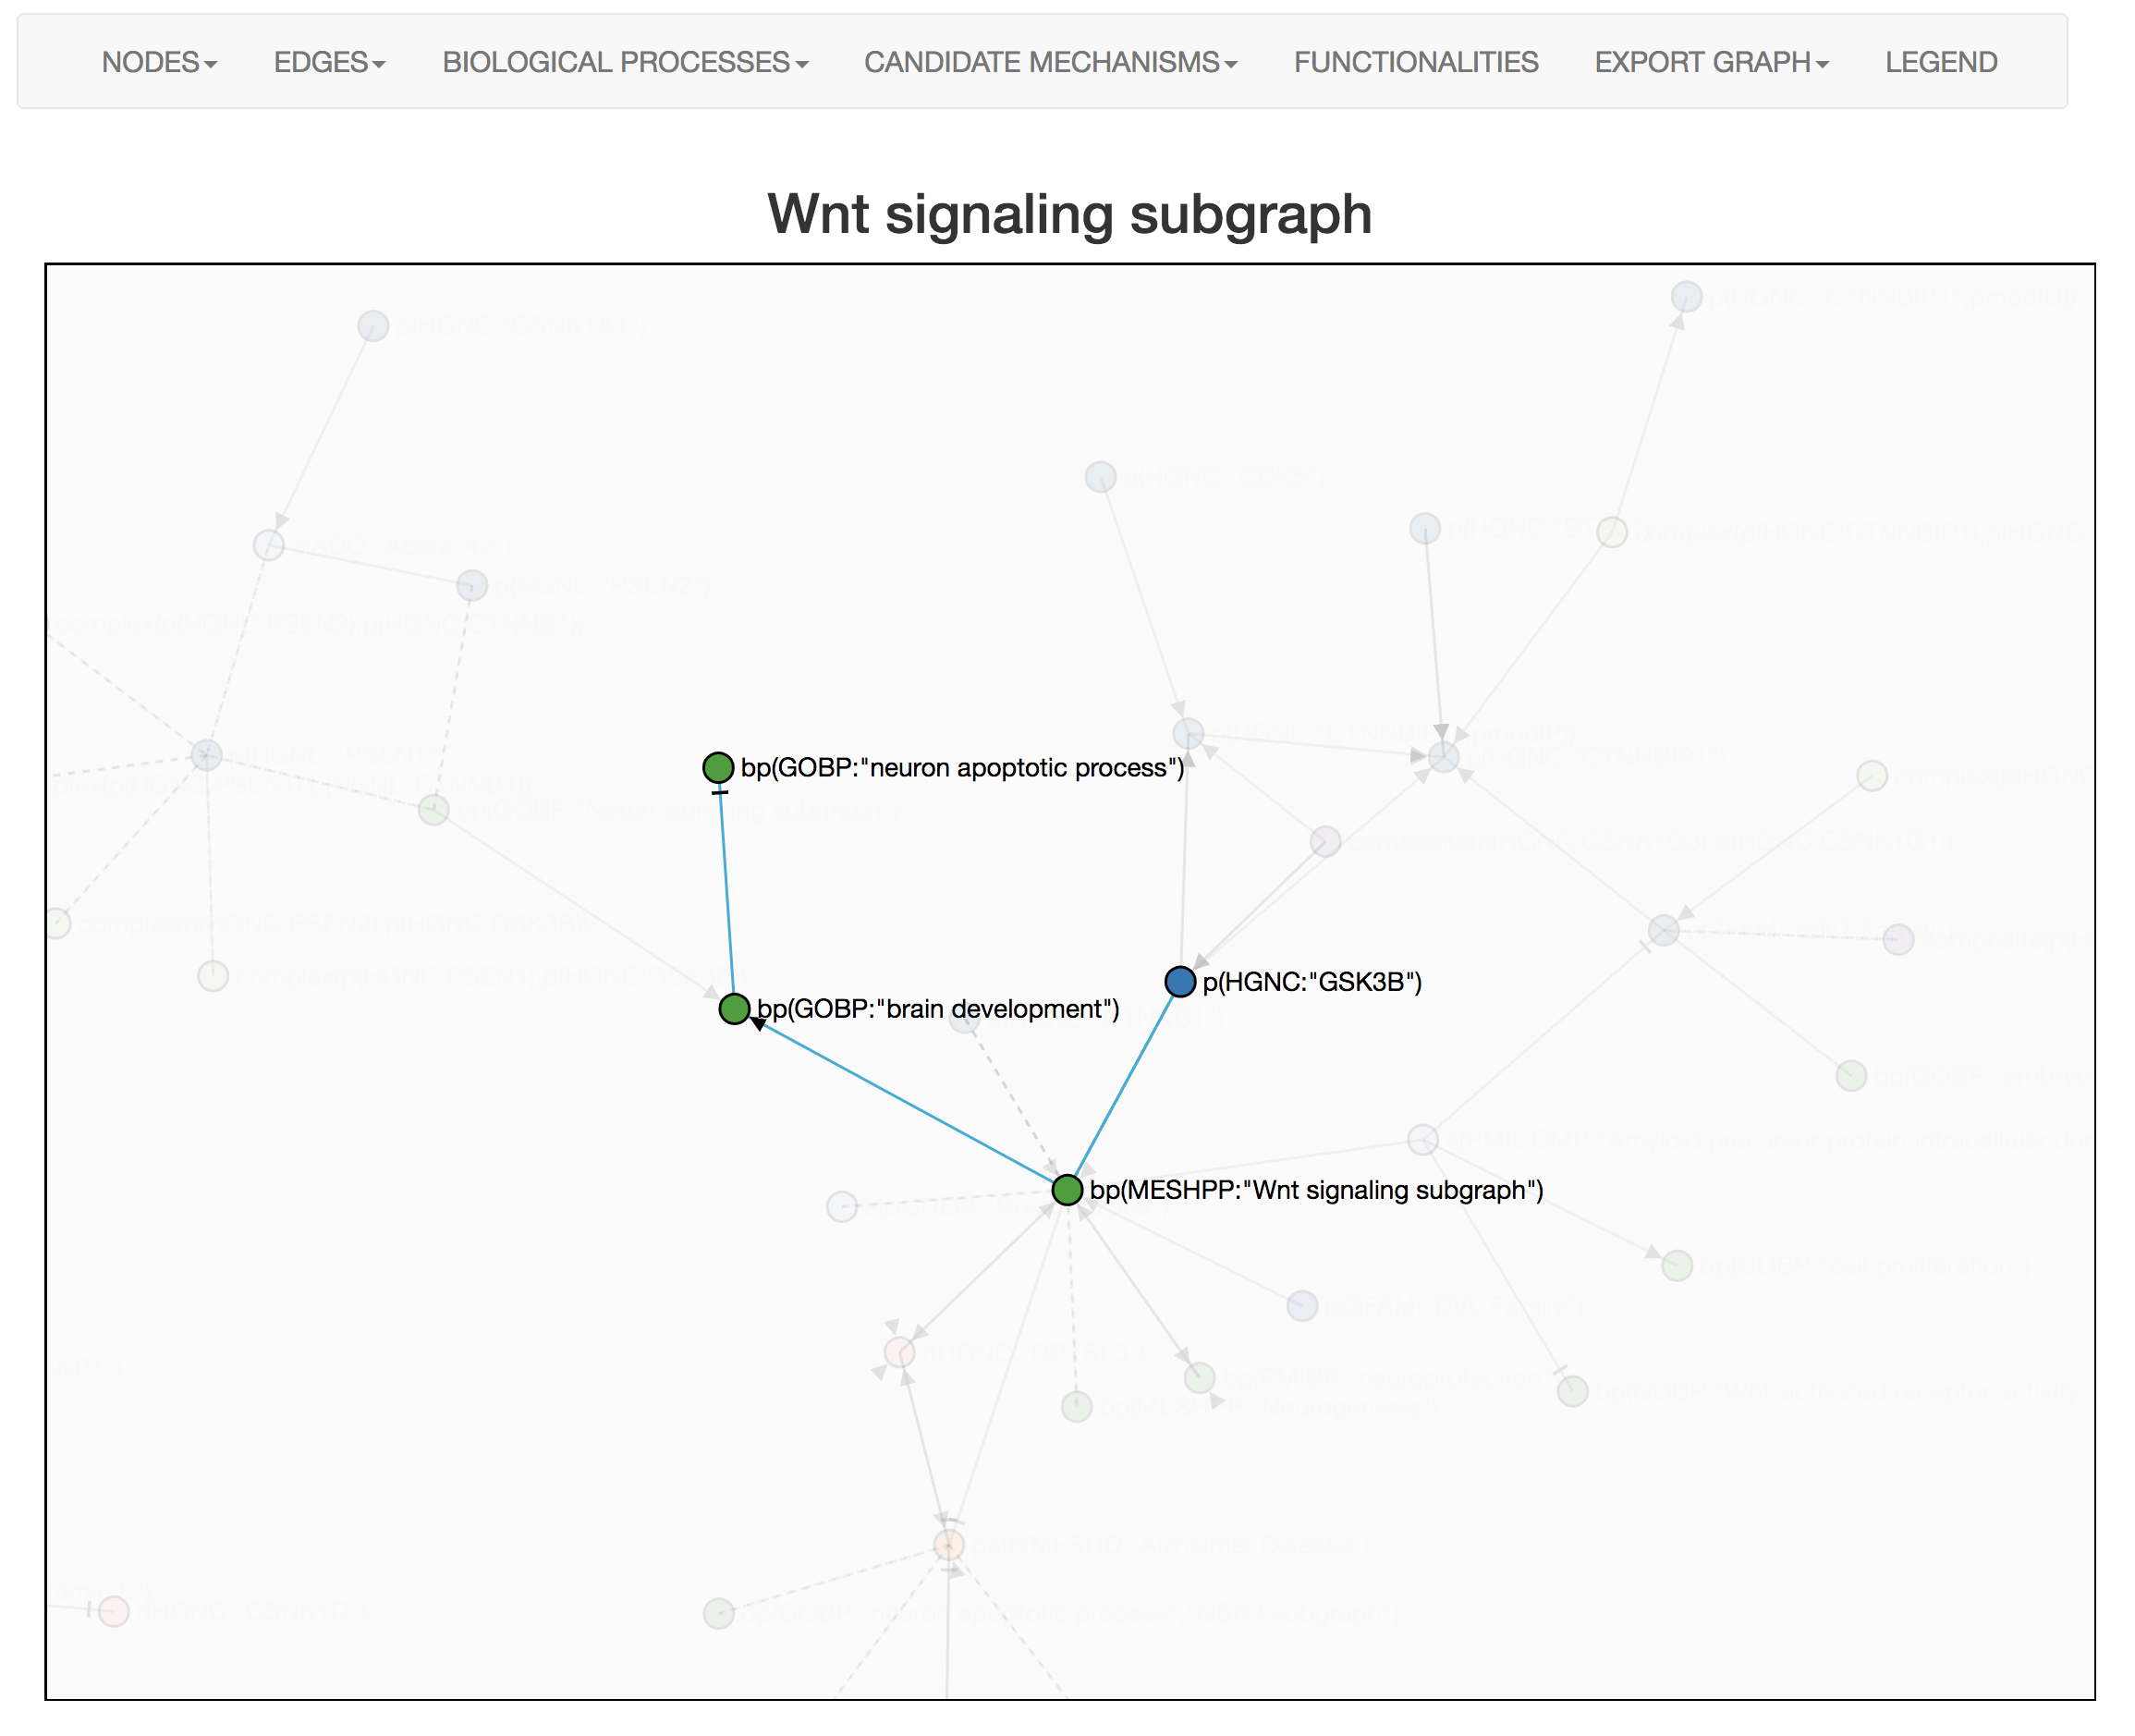
\includegraphics[width=160mm]{images/wnt_neurommsig.png}}
\caption[PyBEL Integration with the NeuroMMSig Mechanism Enrichment Server]{The NeuroMMSig Mechanism Enrichment server uses PyBEL visualization to present a downstream mechanism to the user following multi-modal mechanism enrichment.}
\label{Fig:wnt_neurommsig}
\end{figure}

\begin{figure}
\captionsetup{format=plain}
\makebox[\textwidth]{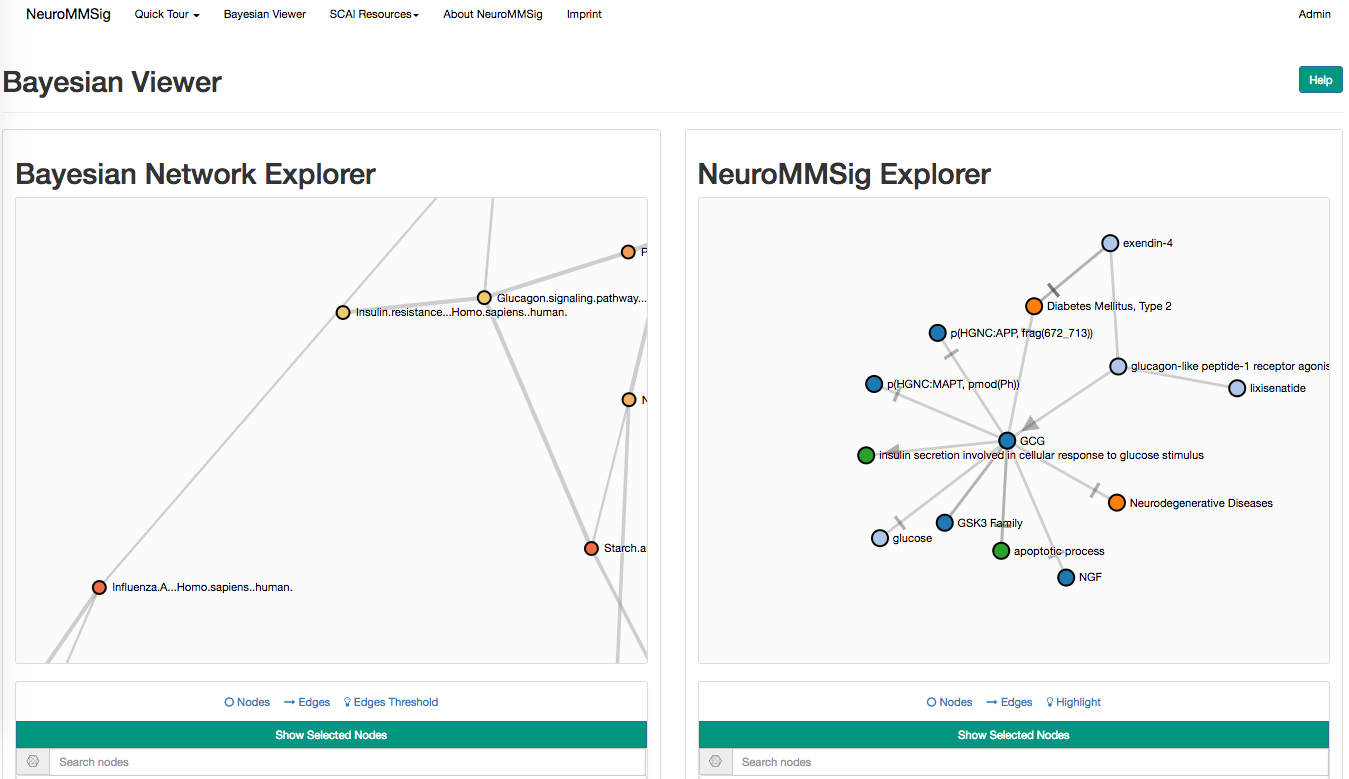
\includegraphics[width=160mm]{images/bayesian_viewer.png}}
\caption[PyBEL Integration with the NeuroMMSig Bayesian Network Explorer]{As an addition to the \ac{NeuroMMSig} Mechanism Enrichment Server, bayesian modeling techniques are used to analyze the dependencies of clinical variables, mapped to \ac{NeuroMMSig} subgraphs, and displayed in a multi-scale exploration environment using the underlying PyBEL visualization system.}
\label{Fig:bayesian_viewer}
\end{figure}

\begin{figure}
\captionsetup{format=plain}
\makebox[\textwidth]{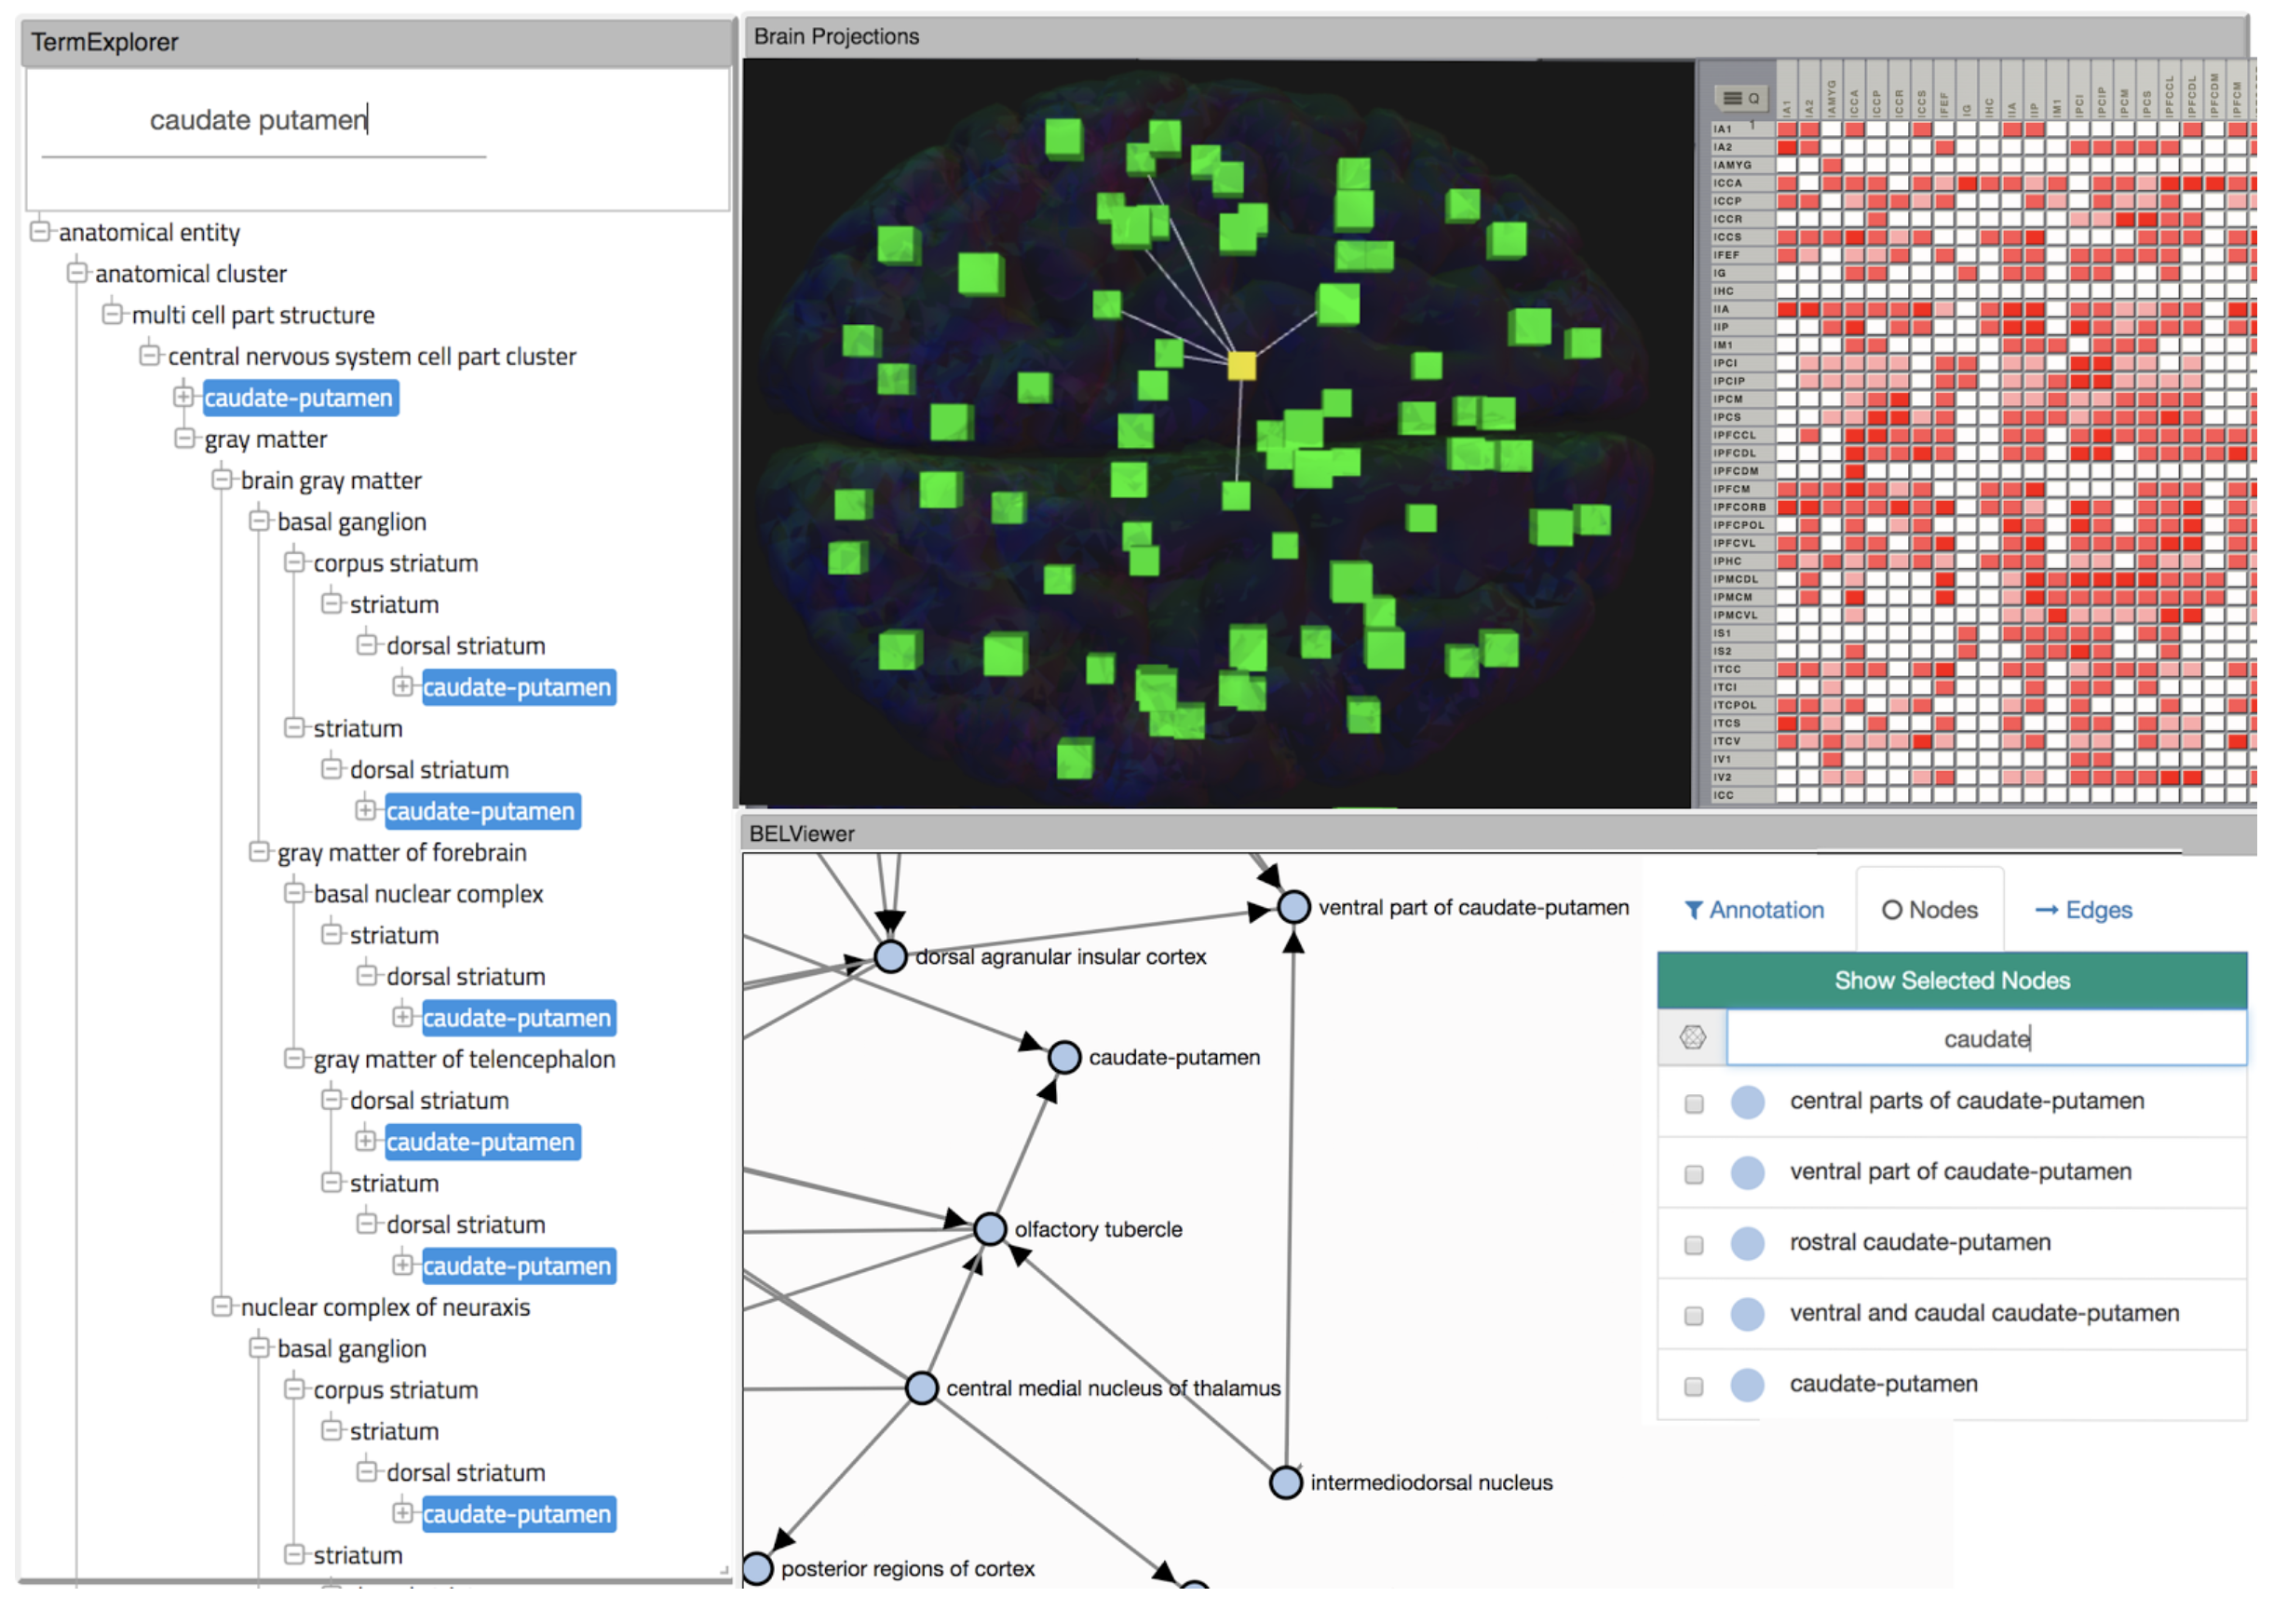
\includegraphics[width=160mm]{images/integration_tvb.png}}
\caption[PyBEL Integration with The Virtual Brain]{The PyBEL visualization system is linked to the tree browser from the Ontology Lookup Service \cite{Cote2006} and connectivity viewer from The Virtual Brain \cite{Leon2013} to allow for interactive exploration of the knowledge related to given brain regions as well as their undirected connectivity or directed projection information.}
\label{Fig:integration_tvb}
\end{figure}

\section{Remarks on Development}

\subsection{Software Stability}

This software was developed under a test-driven development cycle, where extensive unit tests were written to check the stability of the many functions that make up the five components of the software. The procedure for running these tests is encoded with the \verb|tox| build system that is automatically run by Travis \ac{CI} (https://travis-ci.org) upon each push of code to GitHub (https://github.com). The coverage of these tests are then assessed by CodeCov (https://codecov.io).

\subsection{Installation and Usability}

Travis CI also integrates with the "tags and releases" aspect of GitHub to enable automatic build of the code and distribution through PyPI (https://pypi.org), the main packaging system for Python. All relevant information for installation is bundled in the package, so it can be installed with zero configuration on any computer using \verb|pip install pybel| from any terminal, on any operating system, running any modern version of the Python programming language. Finally, the documentation for PyBEL is included in its repository and is automatically built with Sphinx (http://www.sphinx-doc.org) and uploaded to Read the Docs (https://readthedocs.org) upon each push of code to GitHub.

\section{Discussion}

\subsection{Extensibility of Syntax}

Even after its v2.0 update, the \ac{BEL} specification does not yet explicitly specify many concepts in molecular biology such as epigenetic information (e.g. methylation), which is a crucial part of modeling of complex diseases \cite{Irin2015}. The inevitability of language evolution prompted the development of the parser in modules so that new syntax could be proposed and implemented quickly. As a proof of concept, a syntax extension for gene modifications is included in the package by default.

\subsection{Extensibility of Resources}
Historically, \ac{BEL} namespace files have used a custom definition format; but the creation and maintenance of terminologies in the biological domain has tended towards the usage of \ac{OWL}. Furthermore, many namespaces such as dbSNP \cite{Sherry2001} are growing too large to enumerate during semantic integration and validation. The modular architecture of the PyBEL parser enables easy implementation of new definition file formats, external validation services, or even alternative schemes for definition statements to address these issues.

PyBEL introduces syntax for defining namespaces with a consistent pattern using a regular expression to overcome this issue. For these namespaces, semantic validation can be perform in post-processing against the underlying database. The dbSNP namespace can be defined with a syntax familiar to BEL annotation definitions with regular expressions as follows:

\verb|DEFINE NAMESPACE dbSNP AS PATTERN "rs[0-9]+"|

\subsection{Integration of Data}

While \ac{BEL} is often used to formalize knowledge curated from unstructured sources, PyBEL also accommodates the integration of knowledge from structured sources. Existing solutions for resolving equivalences across namespaces have relied on the creation and external hosting of extensive lookup tables. PyBEL could take inspiration from the \ac{OWL} format and enable equivalency information to be directly integrated in a network as edges. 

Again, the parser is extensible enough to implement dedicated syntax for equivalency similar to the standard syntax for gene orthology (\verb|orthologousTo|), protein complex component definitions (\verb|hasComponent|), and protein family membership (\verb|hasMember|). This is realized with the addition of the \verb|equivalentTo| relation, which can be reasoned over using network algorithms directly or collapsed for further use. For example, the fragments produced by amyloid cleavage can be represented in \ac{BEL} with either a protein and fragment combination, or referred directly by its entry in \ac{ChEBI} \cite{Hastings2013}. With the PyBEL extension, this can be written as:

\verb|p(HGNC:APP, frag(672_713)) equivalentTo \|

\verb|a(CHEBI:"amyloid-beta polypeptide 40")|

The hierarchical information encoded in ontologies can also be directly integrated. For example, integrating the \ac{ChEBI} Ontology could allow for reasoning over its multiple functional and structural hierarchies of chemical space. These entries can enable mechanistically-focused chemical repurposing strategies by identifying links between chemical inhibitors in disparate regions of a network \cite{Hastings2013}. 

\subsection{Inaccessible Formats}

Data locked away in other formats such as BioPax and SBML cannot be accessed by PyBEL currently. Development of knowledge assemblers, like \ac{INDRA} \cite{indra}, provide support for import of many formats. PyBEL will enable the import of \ac{BEL} documents much more quickly, and ultimately enable the export of \ac{SBML}. In the future, it would also be useful to develop additional interchange tools for \ac{BioPAX} to \ac{BEL}, but this is a large task that will be limited by the expressibility of each language and the difficult development of a two-way mapping.
There is ongoing work on integrating PyBEL and \ac{INDRA} to immediately make accessible the text mining results from REACH \cite{Valenzuela-Escarcega2015} and TRIPS \cite{Allen2008} as well as the prior knowledge sources assembled for the \ac{INDRA} workflow. Future work is planned to integrate the \ac{BELIEF} workflow \cite{Madan2016} as well.

\subsection{Comparison with Previous Software}

After describing PyBEL, Table 3 is used to make a direct feature comparison with the OpenBEL Framework and bel.rb. While the OpenBEL Framework has some features that are still in develop in the PyBEL ecosystem (see following section on Bio2BEL), PyBEL is the most feature complete and robust option.

\begin{table}
\centering
\caption[BEL Software Ecosystem Comparison]{A comparison of the available software for processing \ac{BEL}. *To the best of our ability, we were unable to install bel.rb using its documentation and unsuccessful in soliciting support through GitHub or OpenBEL's proposed channel of communication on Gitter (https://gitter.im/OpenBEL/chat)}
\label{tab:comparison}
\def\arraystretch{1.1}
\begin{tabular}{p{4cm} p{4cm} p{4cm} p{4cm}}
 & OpenBEL Framework & bel.rb & PyBEL \\
\hline
Programming Language & Java & Ruby & Python \\
Latest Official Release & 2015-06-11 & 1.1.2 - 2017-05-22 & 0.9.0 - 2017-09-19 \\
Installation & Not available on package manager such as brew or apt-get & \verb|gem install bel|* & \verb|pip install pybel| \\
BEL 2.0 Support & No & Experimental & Yes \\
Testing & Yes & Yes & Yes \\
Continuous Integration & No & Yes & Yes \\
Code Quality Testing & No & No & CodeCov and Code Climate \\
Documentation and Tutorials & No & Yes & Yes \\
Command Line Interface & Yes & Yes & Yes \\
Import & BEL Script & BEL Script, RDF & See Table 1 \\
Export & KAM Navigator & RDF & See Tables 1 and 2 \\
Visualization & KAM Navigator & None & See Figures 6-8 \\
Namespace Formats & BELNS & BELNS & BELNS and OWL \\
Compilation Process & Orthology, Named Complexes, Central Dogma & None & Central Dogma \\
Explicit Equivalence Handling & Yes & No & No \\
Extensible Parser & No & No & Yes \\
Programmatic API & No & No & Yes \\
Caching Mechanism & Yes & Yes & Yes \\
Internal DSL & No & Yes & No \\
Ongoing Development & No & No & Yes
\end{tabular}
\end{table}

\section{Conclusions}

\subsection{Applications in Re-curation}
The \ac{NeuroMMSig} knowledge assemblies for \ac{AD} and \ac{PD} had many syntactic, semantic, and biological errors. The PyBEL parser provides a much more useful error analysis than previous software and immediately enabled fixes for many of the syntactic and semantic errors. During this process, a preliminary version control process was implemented to track progress over time. With less than 200 commits and over a period of six months, 5327 of the 8030 errors in the Alzheimer's disease knowledge assembly and 465 of the 1171 errors in the Parkinson's disease knowledge assembly were fixed (Figure 12).

\begin{figure}
\captionsetup{format=plain}
\makebox[\textwidth]{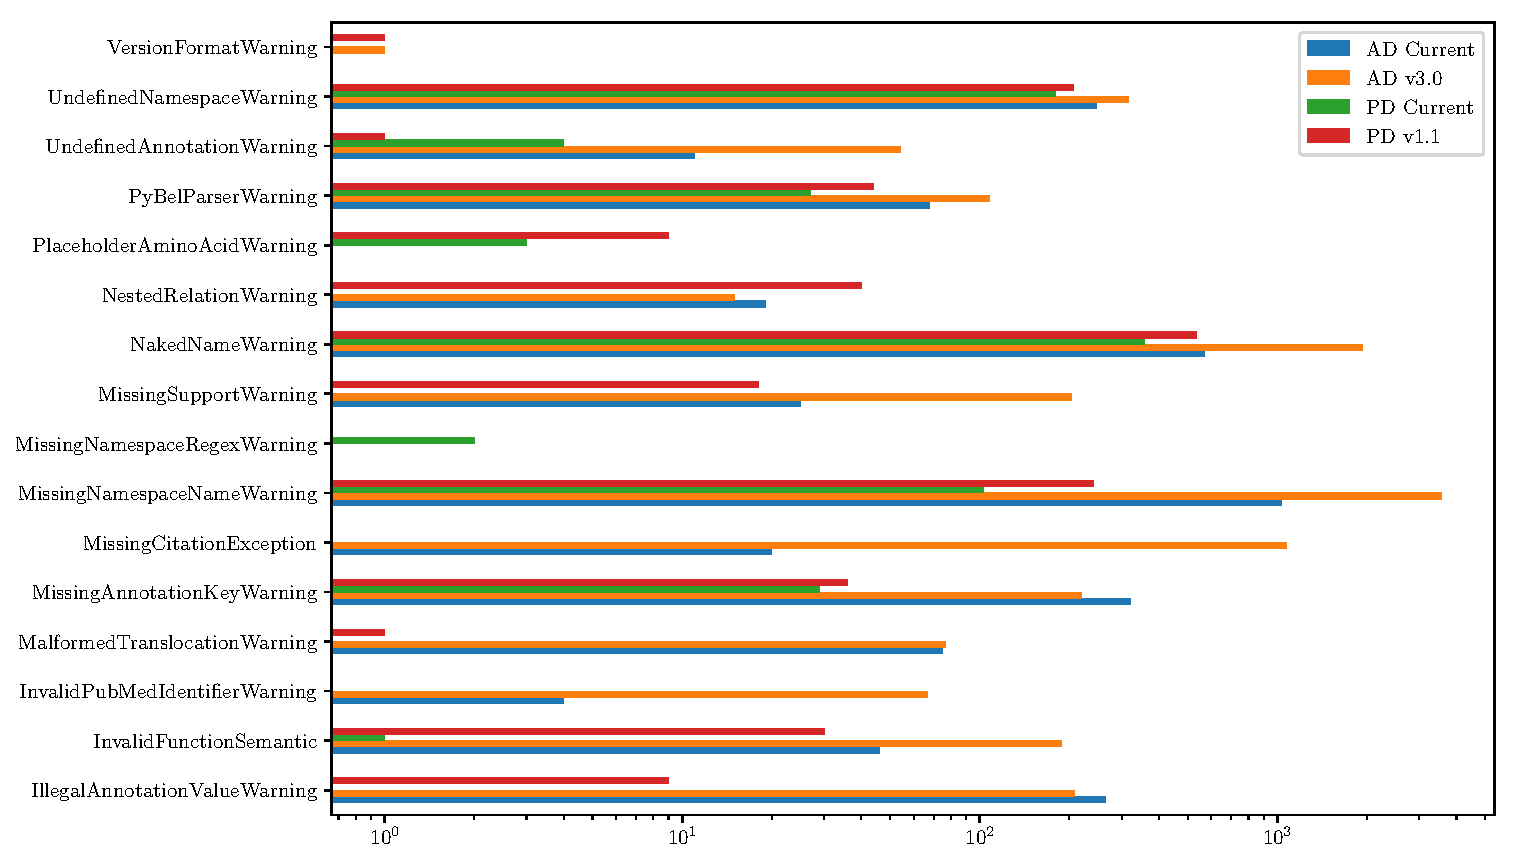
\includegraphics[width=160mm]{images/recuration_bars.pdf}}
\caption[NeuroMMSig Recuration Summary]{The re-curation efforts of the Alzheimer's disease and Parkinson's disease knowledge assemblies showed significant progress after the introduction of PyBEL.}
\label{Fig:recuration_summary}
\end{figure}

Biological problems are much more difficult to detect a priori, but later sections in this thesis describe how integrating data from external sources could allow for an assessment of the "biological grammar" underlying the knowledge assemblies. Future integration with \ac{INDRA} can provide the first steps in automatic analysis of biological correctness using its belief propagation algorithm for quantifying the reliability of statements  based on consensus across text mining and a-priori knowledge bases.

\subsection{Applications in Psychology and Psychiatry}

PyBEL has already been used to stretch the boundaries of manual curation. Projects dealing with anxiety and anhedonia have led to the curation of neuronal connectivity and projects. Other projects dealing with \ac{PTSD} and \ac{TBI} have led to a much larger focus on the curation of biological processes, phenotypes, and clinical measurements. The limited information on the molecular level combine with the focus on non-molecular clinical measurements in these domains motivates the need for integration of new a-priori knowledge bases to assist in the contextualization of new information, critical assessment of the completeness and correctness of new curated material, and new analytical techniques.

\subsection{Future Work}

Integrating chemical information systems like the Comparative Toxicogenomics Database \cite{Davis2017} could enable a previously envisioned chemoinformatics platform \cite{Emon2017} backed by the mechanistic knowledge encoded in \ac{BEL} networks. The extensibility of the network data container enables the integration of relations that are not explicitly defined by \ac{BEL}, such as weighted chemical similarities, for development of novel algorithms and analyses as well as enables the implementation of previously published algorithms for more general use. 


\chapter{Bio2BEL}
\label{ch:bio2bel}

\section{Background on Bio2RDF}

An outline was proposed as early as 1995 for integrating data in the biomedical domain that involved transforming data into a common model, aligning semantically related objects, integrating schemata, and federating data \cite{Davidson1995}. \ac{RDF} has the faculty to address these concerns, and were ultimately realized with the Bio2RDF project, in which multiple biological databases and knowledge bases were serialized to RDF for later integration \cite{Belleau2008}.

As stated before, the expressive power of RDF is counteracted by its lack of domain specificity. While it can be used as an interchange format, it still requires converters to formats for which analytical pipelines have already been developed. Furthermore, the suite of conversion scripts are written in PHP, which has very little traction in the bioinformatics community and therefore is difficult to integrate in pre-existing workflows. This section presents Bio2BEL: a project similar to Bio2RDF for the BEL community to directly the usage of the other tools presented in this thesis.

\section{Generation of Namespace Resources}

There are multiple granularities at which a terminology can be modeled. At the lowest is a vocabulary, in which each term is enumerated and described. Higher is a taxonomy, in which hierarchical relations are expressed. At the highest granularity is an ontology, which contains arbitrary and complex relations.

While it is not the primary goal of knowledge modeling, ontologies can also represent cross-references that connect multiple terminologies that describe the same entities. The most common model for representing ontologies is \ac{OWL} which most commonly uses \ac{RDF} as an interchange format, whose main goal is to provide a platform for semantic integration. This immediately provides ontologies with the facilities developed to support semantic data integration. This is very important in the biomedical domain as rapidly progressing technology frequently results in new experiments and new language for describing biological phenomena.

OWL, and a more domain-specific variant, \ac{OBO}, have been widely adopted by the biomedical domain to structure terminologies and enable semantic integration across knowledge and data sources \cite{Smith2007}. Multiple tools for storing, disseminating, and searching them have been including the Brenda Ontology Explorer \cite{brendaontologyexplorer}, BioPortal \cite{Whetzel2011}, OBO Foundry \cite{Smith2007}, and the EBI \ac{OLS} \cite{Cote2006}.

The semantics of the \ac{BEL} require entities to be identified with a name linked to a namespace. The original framework for handling \ac{BEL} Scripts also provided scripts for gathering different resources (vocabularies, taxonomies, and ontologies) in varying formats and assembling them in a specific namespace file format. One of the advantages of BEL over other systems biology modeling languages is its ability to model knowledge across modes and scales. As it is used to describe new phenotypes, such as the domain of psychiatry, new namespaces must be identified and formatted. Below, two approaches for building new namespaces are described.

\subsection{Direct Generation of Namespace Resources}

The OpenBEL Consortium distributed several scripts that included directives and parsers for acquiring data from multiple knowledge bases and databases and structuring them to BEL namespaces in a reproducible manner. Often, this is necessary to acquire identifiers that are not exported to a standard format like OWL or OBO. Additional scripts were written to improve the reliability of these generators and to convert new namespaces summarized in Table 4.

\begin{table}
\centering
\caption[Direct Namespace Generation]{Data sources for which reusable BEL namespace conversion scripts have been implemented}
\label{tab:direct_namespace_generation}
\def\arraystretch{1.2}
\begin{tabular}{p{5cm} p{10cm}}
Data Source & Description \\
\hline
FlyBase & Drosophila genes and gene products \\
HGNC & Human genes and gene products \\
HGNC Gene Families & Human gene families \\
InterPro & Protein families, domains, and binding sites \\
ChEBML & Experiments describing the effects of chemicals on proteins \\
MeSH Psychiatry and Psychology & A taxonomy of concepts from psychiatry and psychology  \\
dbSNP & \ac{SNP}s \\
miRBase & Premature and mature \ac{miRNA} sequences
\end{tabular}
\end{table}

\subsection{Indirect Generation of Namespace Resources}

BEL namespaces are not generally useful for curators or text-mining platforms to perform named entity recognition. The data sources from which BEL namespaces can be derived often have other rich information (synonyms, hierarchies, and cross-references) that could be structured into an ontology that is more generally useful. 

Some of the namespaces that were originally generated directly by the OpenBEL Framework are derived from ontologies. Since the development of this pipeline, the aforementioned services for hosting ontologies have gained popularity. The \ac{OLS} provides a programmatic \ac{API} from which the terms in a given ontology can be accessed. The source code for this service is available and can be hosted locally. 

The indirect approach uses data sources to build ontologies that can be hosted in \ac{OLS} then to use the \ac{OLS} \ac{API} to iterate over the terms' labels in order to easily convert any ontology to a BEL namespace with a reusable procedure. Already, namespaces in Table 5 have been generated from the publicly available \ac{OLS}. 

\begin{table}
\centering
\caption[OLS-Mediated Namespace Generation]{Ontologies deployed in the OLS from which BEL namespaces have been generated.}
\label{tab:indirect_namespace_generation}
\def\arraystretch{1.2}
\begin{tabular}{p{6cm} p{8cm}}
Ontology & Description \\
\hline
Human Phenotype Ontology & Clinical and phenotypic abnormalities \\
Uber Anatomy Ontology & Anatomical structures in animals
\end{tabular}
\end{table}

As a proof of concept, the data sources in Table 6 have been downloaded and converted to an ontology, deployed on a local \ac{OLS} instance, and converted indirectly to a BEL namespace.

\begin{table}
\centering
\caption[Indirect Namespace Generation]{Data sources from which ontologies have been generated, deployed, and used to generate BEL namespaces.}
\label{tab:indirect_ols_namespace_generation}
\def\arraystretch{1.5}
\begin{tabular}{p{6cm} p{8cm}}
Data Source & Description \\
\hline
\ac{UniProt} & Proteins \\
miRBase & Premature and mature \ac{miRNA} sequences
\end{tabular}
\end{table}

\subsection{Distribution of Namespace Resources}

Each method for downloading, parsing, and generating a namespace is stored as its own self-contained Python package. They share common methods for interacting with the \ac{OLS} in the \verb|ols-client| package. Finally, resources are uniformly deployed and distributed with Artifactory \cite{artifactory}. Common code for uploading to Artifactory is included in PyBEL-Tools. 

\subsection{Discussion Related to Resources}

Not all data sources are amenable to the indirect approach. Infamously, the \ac{MeSH} is a thorough data source that was not developed to accomplish the same goals as ontologies. Therefore, it is incredibly difficult task to map its data to an ontology. Furthermore, the implicit solution to semantic integration that relied on ontologies is not generally applicable. In these scenarios, it is not only necessary to generate a namespace, but also mappings. Previous efforts have relied on lookup tables, but like BEL namespaces, are not generally reusable.

Using ontologies to build namespaces implicitly solves the technical problem of mapping terms from one terminology to another, but this does not necessarily generally solve the biological problem. Mappings between identifiers may have different validity for different applications. While it is often convenient for biological literature to name proteins by their genes' names, this can create ambiguity for genes that produce multiple products in the cases of differential splicing and post-transcriptional modification. For example, in some simplistic domains, it is possible to map HGNC gene identifiers to \ac{UniProt} protein identifiers. However, when modeling complex phenotypes that rely on this mechanism, this mapping cannot be used.

\section{Knowledge Integration}

Knowledge can be represented as statements each consisting of a subject, predicate, and object. As knowledge is assembled, the object of one statement may be the subject of another. This process implicitly builds a knowledge network over which reasoning and inference may be performed. Two general purpose technical solutions for storing statements are relational databases and \ac{RDF}.

A relational database allows for similar statements, often ones with the same types of subjects, same types of objects, and same predicates, to be stored in tables. Each row represents one statement, where the subject and the object are assigned a column and additional columns can represent the metadata associated with the assertion of the statement. While their structure is explicitly, relational databases have the disadvantage of becoming large and complicated when representing many types of knowledge. As a result, many knowledge bases are disparate. Further, the management systems underlying relational databases are generally not amenable to federation.

One solution to this problem is to expose the database through \ac{API}s that can be queried from external services to enable federation of multiple relational databases. A popular solution is the \ac{REST} \ac{API}, but to integrate many data sources might require multiple queries, which can put a strain on technical systems. A newer solution is \ac{GraphQL}, which attempts to provide an abstraction layer between relational databases and \ac{REST} \ac{API}s to handle federation more efficiently.

An alternative medium to relational databases entirely is \ac{RDF}, in which all statements are explicitly stored as triplets of subject, predicate, and object in an alternative database management system called a triple-store. The underlying data can be exposed with a \ac{SPARQL} endpoint, which enables the statements to be queried. Further, it directly enables path queries to enable reasoning and inference. \ac{RDF} was developed to enable federation directly using \ac{SPARQL} endpoints from multiple data sources. It also does not need a well-defined schema in the same way a relational database does. This is both a blessing and a curse; new data can be added quickly, but the lack of structure makes it both technically and pedagogically difficult to make pointed queries.

\subsection{Utility of Biological Expression Language}
Because relational databases and \ac{RDF} are general solution for storing knowledge, they are unaware of the domain-specific needs of knowledge representation and storage in the biomedical domain. Among other modeling languages and formats for systems and networks biology, \ac{BEL} is an apt medium for storing structured knowledge extracted from the literature because it enables inference and reasoning over varying topologies of the resulting networks and also a serialization format for structured knowledge bases to enable integration in a domain-specific medium. It is a solution to overcoming the technical limits imposed by RDF on representing relation metadata and the technical limits imposed by relational databases in constructing and querying networks.

BEL is commonly used for manual curation in a specific disease area. Integrating prior knowledge sources to these networks provides context not only to assist the curator in their understanding of the biological knowledge surrounding their curation, but also allows for automatic enrichment, improved reasoning, and a further step towards building a support system for data interpretation. 

Among the most easily integrable structured knowledge formats in BEL are taxonomies, ontologies, and networks. Taxonomies and ontologies directly provide the facility for reasoning and inferences of new knowledge. Networks, such as bipartite \ac{SNP}-disease, chemical-gene, or gene-pathway networks, can be directly integrated in \ac{BEL}. Even networks created by statistical calculations can be added to \ac{BEL} networks to investigate their explanatory power. For example, the \ac{eSNPO} provides statistical associations between \ac{SNP}s and \ac{GO} biological processes. While these don't have mechanistic support, they can provide additional insight and allow for more informed hypothesis triage in network analysis. Here, two approaches for serializing structured knowledge sources to \ac{BEL} are described.

\subsection{Direct Generation of Knowledge Resources}

While structured, the formats in which knowledge is stored varies by domain. For example, ChEBML \cite{Gaulton2012} is distributed as a relational database, while BKMS-react \cite{Schomburg2017} uses a table with specifically formatted entries to describe reactions. For each source in Table 7, a reusable Python library that downloads, structures, queries, and serializes \ac{BEL} was developed.

\begin{table}
\centering
\caption[Direct Knowledge Resource Generation]{Knowledge bases for which reproducible BEL serialization procedures were implemented.}
\label{tab:direct_knowledge_generation}
\def\arraystretch{1.5}
\begin{tabular}{p{25mm} p{20mm} p{45mm}}
Knowledge Source & Type & Description \\
\hline
ChEMBL & Relational Database & Chemical inhibition and binding of enzymes \\
HGNC Orthologies & Tabular & Gene orthology mappings between human, rat, and mouse \\
BKMS-react & Tabular & Biochemical reactions and catalytic enzymes \\
\ac{eSNPO} & Tabular & Relations between \ac{SNP}s and biological processes
\end{tabular}
\end{table}

\subsection{Indirect Generation of Knowledge Resources}

Serializing knowledge to \ac{BEL} is not generally useful outside of the domain of tools directed towards \ac{BEL} networks.  The knowledge bases from which \ac{BEL} can be derived often have other rich information that is not appropriate for \ac{BEL} that could be structured in other knowledge representation models such as \ac{OWL}. For these cases, the parser and serializer were separated in order to build an intermediate relational database. These have the added benefit of being queryable through \ac{SQL} or exposed with RESTful \ac{API}s for large data sets across networks. Finally, these database schemes have the additional benefit of providing a formalism for the knowledge before serializing it to BEL. As a proof of concept, packages have been developed for the parsing, database storage, and BEL serialization for sources listed in Table 8.

\begin{table}
\centering
\caption[Indirect Knowledge Resource Generation]{Knowledge bases for which an intermediate solution for downloading, parsing, and modeling data were used to facilitate the development of reproducible BEL serialization procedures.}
\label{tab:indirect_knowledge_generation}
\def\arraystretch{1.5}
\begin{tabular}{p{25mm} p{20mm} p{45mm}}
Knowledge Source & Type & Description \\
\hline
Comparative Toxicogenomics Database & \ac{XML} & Relations between chemicals, genes, pathways, and phenotypes \\
InterPro & Hierarchy & Protein Family Hierarchies \\
HGNC Gene Families & Tabular & Gene Family Hierarchies
\end{tabular}
\end{table}

\subsection{Discussion Related to Knowledge Resources}

Many more knowledge bases and data sources exist that could be integrated with \ac{BEL}. For example, \ac{miRNA}-Target interactions stored in mirTarBase \cite{Chou2016} could provide insight to the complex regulation patterns that applies to complex diseases. Other sources of knowledge could be extracted from data-mining pipelines, such as linkage disequilibrium block analysis, gene co-expression analysis, and perturbagen-based differential gene expression analyses to provide additional support to elucidate mechanistic insight from increasingly complicated and large knowledge assemblies.


\chapter{PyBEL Tools}
\label{ch:pybel_tools}

The following section describes a subset of the functions and workflows that have been developed to assess, enrich, and analyze knowledge assemblies parsed by PyBEL. All code is made available as open source and stored in the PyBEL Tools repository (https://github.com/pybel/pybel-tools) on GitHub. Like PyBEL, it is thoroughly documented as to allow for the community to build upon it.

\section{Critical Assessment of Networks}
Before knowledge assemblies can be used to help interpret data, their validity and robustness must first be quantified. While many dimensions can be explored during this quantification, this section places focus on the identification of biological network motifs that indicate inconsistencies in the knowledge assembly. Network motifs have been studied in the context of transcriptional and phosphorylation networks \cite{Alon2007} and already provide insight to the biological activity. As knowledge networks add the heterogeneity of edges including correlative relationships, many new motifs must be identified and their effects inferred. This section presents the first portions of a taxonomy for network motifs in knowledge assemblies, interpret their effects, and use them assess the \ac{NeuroMMSig} knowledge base.

\subsection{A Taxonomy of Knowledge Assembly Motifs}

The first and most simple motif is a contradictory pair. These occur when there exist multiple edges between a given source and target that have conflicting relations, such as increases vs. decreases. However, contradictory pairs are not canonically invalid. They may arise from the effects of the biological context under which different relations were observed. These cases must be carefully considered.

There are many aspects that can be considered to resolve conflicts that cannot be explained by different biological scenarios. First, the date of publication can be considered. The most recent publication is most likely to have made use of other knowledge available to researchers, and be more right. Alternatively, if many publications were made with conflicting views in a short amount of time, the impact factor of the corresponding citations' journals can be considered.  

While there exists a single motif for identifying contradictory pairs, multiple motifs comprise the set of contradictory triplets. The algorithms that identify these triangles within a network come from a deep graph theoretic background to identify logically inconsistent relations. Because BEL knowledge graphs contain both causal and correlative relations, they can be analyzed jointly. The most simple is a mutually unstable triplet, which occurs when entities A, B, and C all negatively correlate with each other. Similarly, separately unstable triplets occur when A positively correlates with both B and C, but B and C are negatively correlated. Three more triple types are identified where a mix of  correlative and causal relations do not match: increase mismatch triplets, decrease mismatch triplets, and jens triplets.

Alternatively, stability analysis can be conducted to identify elements that are likely to be regulated by other parts of a system. These elements are particularly interesting because of the high impact that any given edge could have that connects to it. There are two types of unstable pairs: chaotic pairs, where A and B both increase each other and dampened pairs, where A and B both decrease each other. The same logic extends to chaotic triplets and dampened triplets. Interestingly, analyses of many knowledge assemblies seldom identified dampened triplets; possibly indicating their biological novelty. Chaotic and dampened cycles of length 4 and above are not identified, because the average number of possible connections at those lengths makes qualitative biological interpretation prohibitively difficult. 

Table 9 presents statistics over the occurrence of various network motifs in the three knowledge assemblies produced during the AETIONOMY project. While each case, such as mutually unstable triples, might be interesting, this provides direct insight into the large amount of effort necessary to investigate each unstable motif and motivates the further development of automated approaches for quantifying the robustness of a given knowledge assembly.

\begin{table}
\centering
\caption[Stability Analysis of NeuroMMSig]{Stability analysis statistics over the AETIONOMY knowledge assemblies for Alzheimer's disease, Parkinson's Disease, and Epilepsy. The ratios suggest that the relative counts of each network motif are not similarly correlated with network size or density. }
\label{tab:stability}
\def\arraystretch{1.5}
\begin{tabular}{p{55mm} p{25mm} p{25mm} p{25mm}}
 & \ac{AD} Knowledge Assembly v4.0.3 & Epilepsy Knowledge Assembly v1.1.2 & \ac{PD} Knowledge Assembly v1.1.1 \\
Chaotic Pairs & 56 & 12 & 16 \\
Chaotic Triples & 115 & 27 & 11 \\
Contradictory Pairs & 68 & 18 & 26 \\
Dampened Pairs & 7 & 2 & 4 \\
Dampened Triples & 1 & 0 & 2 \\
Decrease Mismatch Triples & 20 & 0 & 6 \\
Increase Mismatch Triples & 51 & 4 & 20 \\
Jens Unstable Triples & 657 & 153 & 85 \\
Mutually Unstable Triples & 2 & 0 & 7 \\
Regulatory Pairs & 19 & 9 & 15 \\
Separately Unstable Triples & 16 & 0 & 16
\end{tabular}
\end{table}

\subsection{Discussion}

As data integration projects like Bio2BEL make more data accessible during analysis, further plausibility and stability checks can be performed. One would be to integrate the data from \ac{UniProt} for each function and traverse the Gene Ontology molecular function annotations to identify properly annotated activities and flag improperly annotated ones to be either proposed as new, or fixed. Another example would be to check that protein and gene modifications are annotated properly using \ac{UniProt} and dbSNP, respectively. Adding additional checks using prior knowledge makes \ac{BEL} curation much more accessible to curators with less biological knowledge and also text mining systems that currently have less biological intuition.

\section{Survey of Algorithms}

Algorithms for analyzing pathways and networks can be categorized into three main categories: \ac{ORA}, \ac{FCS}, and \ac{PT} \cite{Khatri2012}. Over-representation analysis often focuses on the number of differentially expressed genes present or absent in a gene set compared to chance, while functional class scoring is less susceptible to large effects and considers the aggregate of groups of small effects. Pathway topology finally considers the biological relations between members of the pathway during analysis.

Furthermore, there is a distinction between methods that rely on the assumption that protein activities are correlated with their corresponding \ac{mRNA}s' expression changes (forward reasoning) versus the effect that upstream controllers of \ac{mRNA} expression have (backwards reasoning) \cite{Martin2014}

These algorithms have been developed for a wide variety of applications, data formats, and graph types. While many are heterogeneous, below are the most notable algorithms specific to networks from knowledge assemblies encoded in \ac{BEL}.

\subsection{Reverse Causal Reasoning}

Reverse causal reasoning (\ac{RCR}) is an approach to identify the upstream controllers of biological patterns measured in an experiment; often differential gene expression experiments between healthy and diseased patients. First, large knowledge assemblies are dissected into smaller hypothesis networks with one upstream node with multiple outgoing causal relations to target nodes represented by the experimental data set. Each hypothesis network is scored by its concordance between the observed up- and down-regulations of targets nodes to the sign of the causal relation and by its richness, or the explanatory power of the hypothesis network \cite{Catlett2013}. An example hypothesis network is shown in Figure 13.

\begin{figure}
\captionsetup{format=plain}
\makebox[\textwidth]{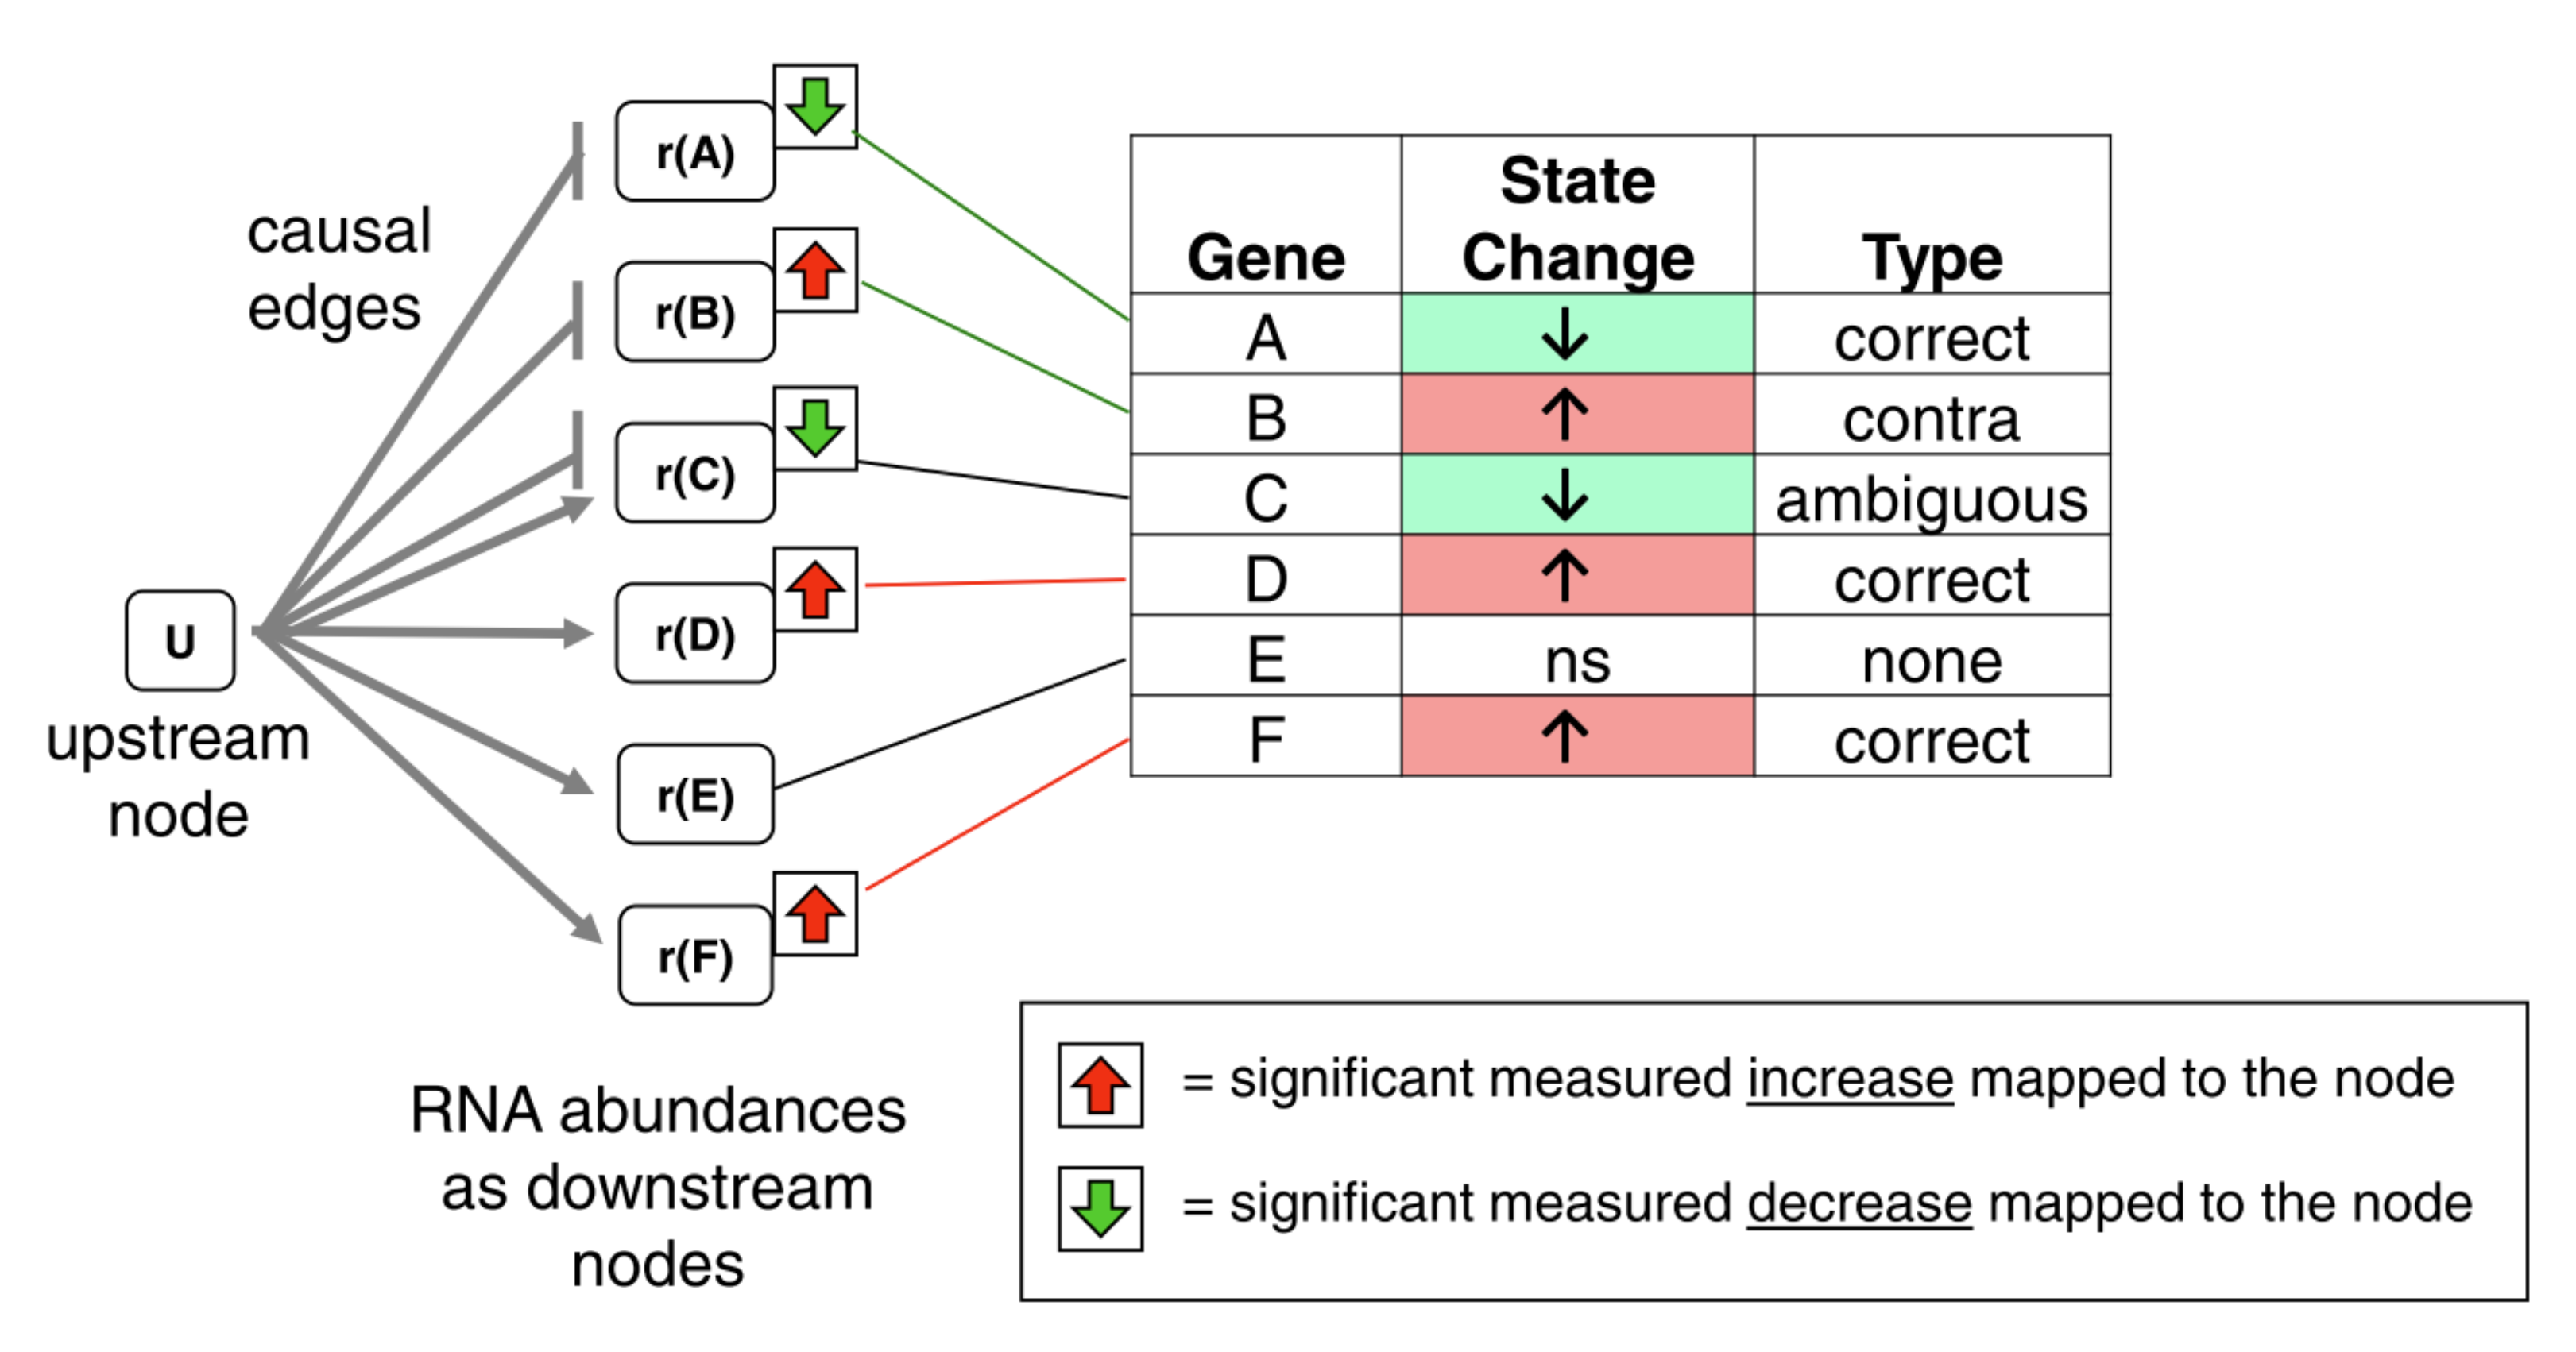
\includegraphics[width=160mm]{images/rcr_schematic.png}}
\caption[A Schematic Diagram of \ac{RCR}]{An example hypothesis network. Target nodes are counted as correct if they have a decreasing relationship and down-regulation, or an increasing relationship and up-regulation. Target nodes with multiple conflicting relationships are marked as ambiguous. Finally, target nodes are counted as incorrect if they have a mismatch between an increasing relationship and down-regulation, or a decreasing relationship and up-regulation. Adapted from \cite{Catlett2013}.}
\label{Fig:rcr_schematic}
\end{figure}

\subsection{Network Perturbation Amplitude}

While \ac{RCR} gives preliminary insights to significant biological controllers, it mostly ignores the topology of signaling, regulatory, and other causal networks that can be represented in knowledge assemblies (Figure 14). The \ac{NPA} measures the aggregated effect explained by the controller layer with reference to a given node with respect to their downstream nodes. Two complementary statistics for the effect of permutations of the upstream layer and downstream layer allow for further insight to the validity of \ac{NPA}s as a hypothesis generation mechanism \cite{Martin2014}.

\begin{figure}
\captionsetup{format=plain}
\makebox[\textwidth]{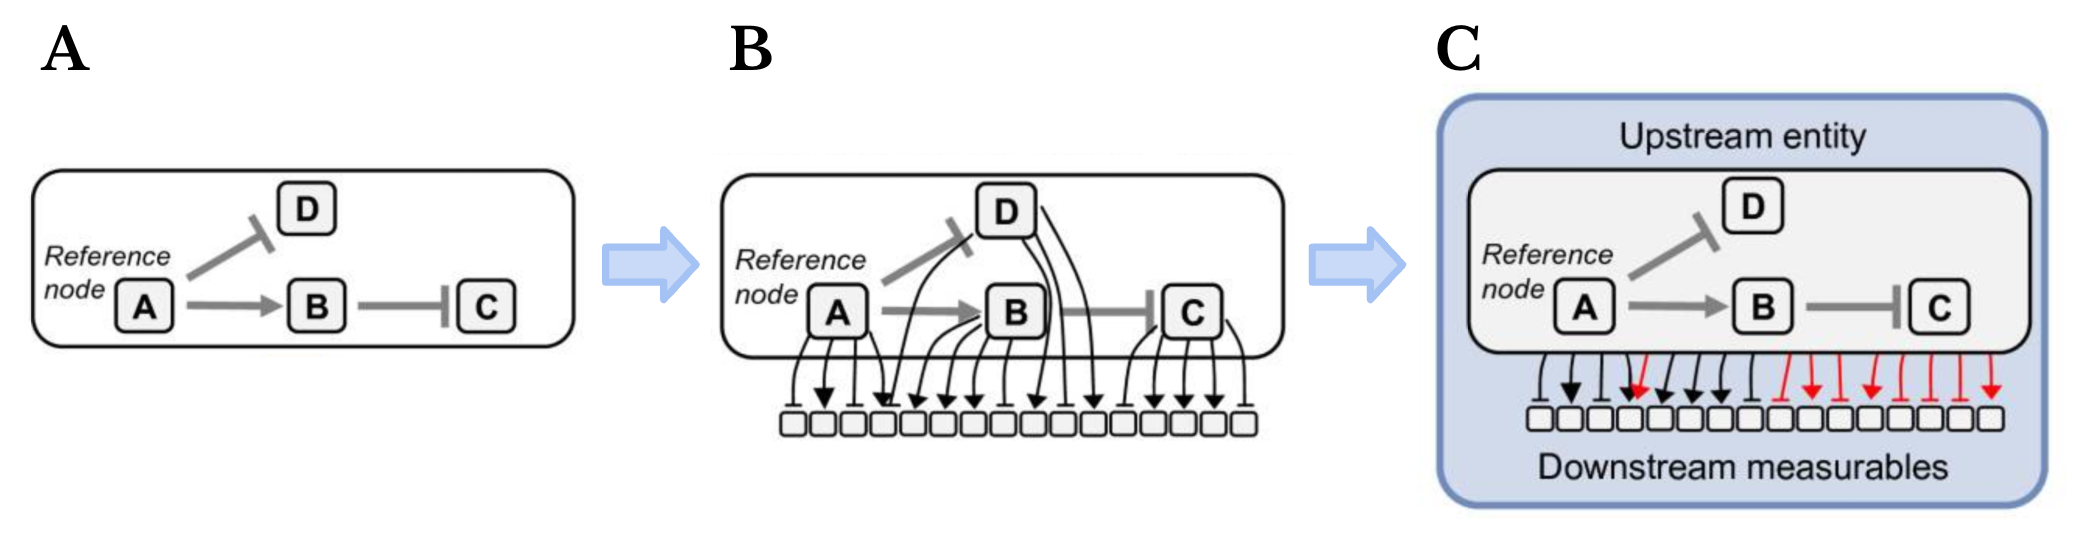
\includegraphics[width=160mm]{images/npa_schematic.png}}
\caption[Hypothesis Network Generation for Network Perturbation Amplitude]{Creation of hypothesis networks that accounts for the topology and interactions of  upstream controller layer with respect to a reference node A), their individual effects on the downstream layer B) and their combine effect C). Adapted from \cite{Martin2012}.}
\label{Fig:npa_schematic}
\end{figure}

\subsection{Sampling of Spanning Trees}

While \ac{NPA} enables more informed analyses than \ac{RCR}, its mathematical basis limits the topologies of knowledge networks that can be used to those with causal consistency. In these networks, all paths from one node to another result in the same aggregated effect of increases and decreases. An additional approach in Figure 15 for \ac{SST} with random walkers eliminates inconsistencies and can be aggregated over multiple trials to assign \ac{NPA} scores to networks that were otherwise inconsistent \cite{Vasilyev2014}. 

\begin{figure}
\captionsetup{format=plain}
\makebox[\textwidth]{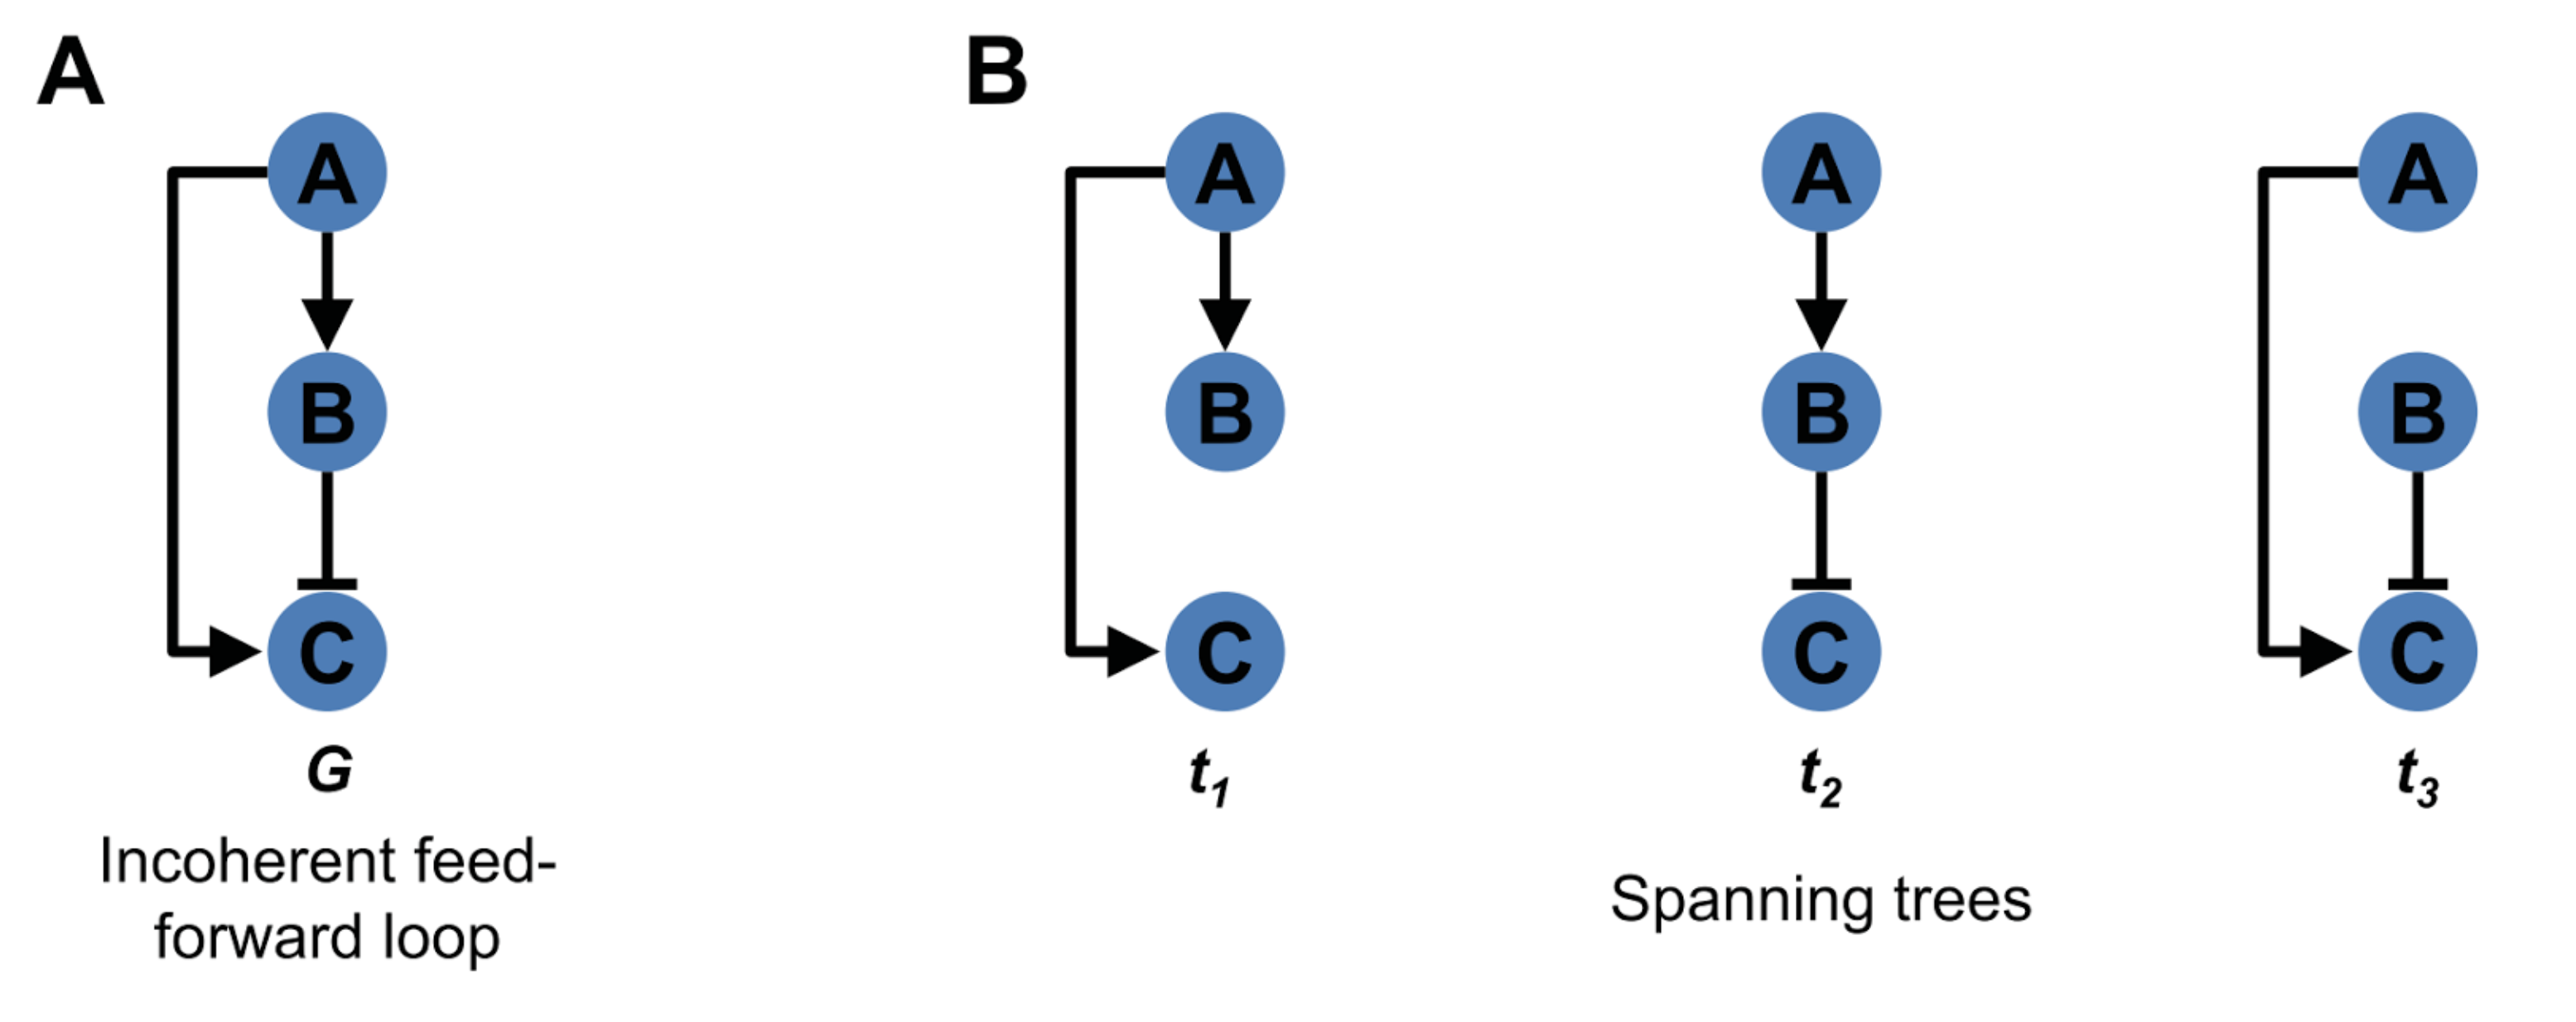
\includegraphics[width=160mm]{images/sst_example.png}}
\caption[Decomposition of Spanning Trees]{An example decomposition of a small causally inconsistent network A) to its spanning trees B)\cite{Vasilyev2014}.}
\label{Fig:sst_schematic}
\end{figure}

\subsection{Unsolved Issues}

While these algorithms already provide significant insight, they still have unresolved issues. For example: they require prior definitions of the upstream controller layer subnetworks; they do not address other exotic network motifs such as contradictions; and they do not take advantage of the vast assembly of correlative relationships. Further, there is generally a low coverage of nodes present in data sets within knowledge assemblies.

As mentioned before, these algorithms were developed for domains (oncology, immunology, etc.) that are rich in molecular data and mechanistic knowledge. For disease areas such as neurodegenerative diseases, molecular data (e.g., microarray, \ac{RNA}-seq) are not often available for the most applicable cells or tissues because of the practical difficulty of acquiring samples. It follows that context-specific knowledge is also much more sparse; and inference from other contexts (such as animal models) is much less reliable.

While backwards reasoning overcomes the issues with interpretation that are posed by forwards reasoning, the insufficient knowledge and data in neurodegenerative diseases makes this revelation much less useful. 

The experimental data available in for this field and other complex diseases are often multi-modal and multi-scale, prompting the development of new methods. Many of these experiments can only be connected to current knowledge assembles through correlative relationships, such as the associations between single nucleotide polymorphisms (\ac{SNP}s) and clinical phenotypes such as neuroimaging and gene expression. 

\section{A Priori Network Augmentation}

This section first describes pipelines that make biological knowledge assemblies more usable that rely on prior knowledge from the biomedical domain. Before developing analytical algorithms, it is first necessary to consider pipelines that improve the features of currently existing networks. After, an algorithm for generating upper layer controller networks is proposed and an alternative heat-diffusion method that is better able to accommodate heterogeneous experimental data. 

\subsection{Connecting Disconnected Components}

The GABA Subgraph in the Alzheimer's disease knowledge assembly has five disconnected components. While these can be inspected manually and the gaps can be filled, this becomes a daunting task for the set of 128 subgraphs in NeuroMMSig. PyBEL can be used to build queries that automatically expand and enrich graphs in order to create an environment in which disparate knowledge can be assembled to elucidate mechanistic understanding. Below, a procedure for filling in the holes in a subgraph is outlined. 

First, the central dogma is inferred. This ensures the existence of the corresponding RNA for proteins, and the corresponding genes for each \ac{RNA} and \ac{miRNA}. Doing so already connects the subgraph containing the relations describing how estradiol affects the expression of GABRA4 and GABR3 \ac{mRNA} \cite{Noriega2010} to another component that describes the functional impact of their translated proteins on other proteins and biological processes. After this process, four components remain.

Next, unqualified edges are enriched. This method reasons over nodes for which assertions can automatically be presumed. Relationships describing the different types of variations on genes and proteins (epigenetics, mutations, and post-translational modifications) are able to connect the GRIN2B node that is important in one large component to the phosphorylated GRIN2B node in another network. Because \ac{BEL} represents knowledge assemblies and not necessarily mechanistic models, these pieces of information can come from multiple curators without mutual knowledge. After this process, two components remain.

Of the two components, there is one large component and one small component, consisting only of cAMP catabolic process and GABBR2. While they are not yet automatic, further knowledge-based approaches can be used to connect GABBR2 to GABBR1 in the large component using resources like \ac{HGNC} Gene Families \cite{Gray2015}, InterPro \cite{Finn2017}, or PFAM \cite{Finn2016}. This is valuable because hierarchical knowledge sources like these can be used to reason over the network, like using the knowledge that GABBR2 decreases the cAMP catabolic process  \cite{Massone2011} to assert that GABBR1, the other member of the GPCR family 3, GABA-B receptor (IPR001828), shares the same activity. While this knowledge does not exist in the assembly, literature search also notes several connections between GABBR1 and cAMP signalling \cite{Frere2004,Palmer2005}.

\subsection{Subgraph Membership Inference}

While connecting components is important, it would also be useful to identify and add edges that should belong to the GABA subgraph but do not already. The first method would be to identify and edges occurring between nodes in the subgraph that are not already present, and add them. Next, this procedure can be continued to identify nodes that have edges to multiple nodes already in the subgraph. To reduce false positives, nodes added this way must both be the target of a causal relationship from a node in the subgraph and also have a causal effect on another node in the subgraph.

Finally, to improve viewability, two additional filters are provided. First, a filter for pathologies is used to remove them. This is useful since most pathologies are "super nodes" in knowledge assemblies and have numerous and often uninformative correlative relationships. Next, the central dogma is collapsed such that genes, \ac{RNA}s, and proteins are all shown as one node. While this limits the mechanistic explanatory power of a visualization, it removes a significant amount of visual clutter. 

\subsection{Pipeline Building}

It may be reasonable for viewing purpose to additionally collapse nodes representing modifications to their reference node as well. The submodule \\ 
\verb|pybel-tools.mutation| contains large library of functions that can be chained together either manually, or with a pipeline builder to promote reusability by allowing uses to save their workflows and reuse them. 

\section{Data Driven Analysis}

\subsection{Unbiased Candidate Mechanism Generation}

There are many terms used to describe portions of biological networks including pathways, mechanisms, subgraphs. They all comprise of individual interactions that accumulate to a more complex function. Often, an interaction may be part of multiple of these features. Knowledge bases like \ac{KEGG}, Reactome, and WikiPathways organize interactions into pathways; but they all suffer from bias in the literature and from the knowledge of their curators. This section presents an algorithm for generating unbiased candidate mechanisms from a given knowledge assembly. The method is then compared to the NeuroMMSig knowledge base to identify its ability to reproduce dogmatic subgraphs and identify areas of the underlying knowledge assemblies that have yet to be annotated.

In biomedical knowledge assembly across scales, biological processes represent entire subnetworks of causal interactions through both time and space. The \ac{NeuroMMSig} knowledge base captures associative, correlative,  and causal relationships between genes and gene products and biological processes directly in BEL. Because biological processes implicitly represent functional subnetworks, they are an appealing starting point for automatically unbiased generating candidate mechanisms to be used by other algorithms. 

The upstream controllers of biological processes provide direct insight to their functional impacts across scales. Therefore, the simple algorithm for generating candidate mechanisms that are unbiased by the dogmatic  takes the causally upstream controllers of a biological process, their upstream controllers, and all internal causal edges between them as a candidate mechanism. This method is thresholded at an expansion of two neighborhoods, but could easily be modified to choose larger or smaller lengths.

\subsection{Comparison to NeuroMMSig Knowledge Base}

This method was applied to the NeuroMMSig Alzheimer's disease knowledge assembly for each biological process. After, the resulting candidate mechanisms are compared to the NeuroMMSig subgraphs. First, the landscape of biological process membership in each subgraph is summarized with Figure 16. 

\begin{figure}
\captionsetup{format=plain}
\makebox[\textwidth]{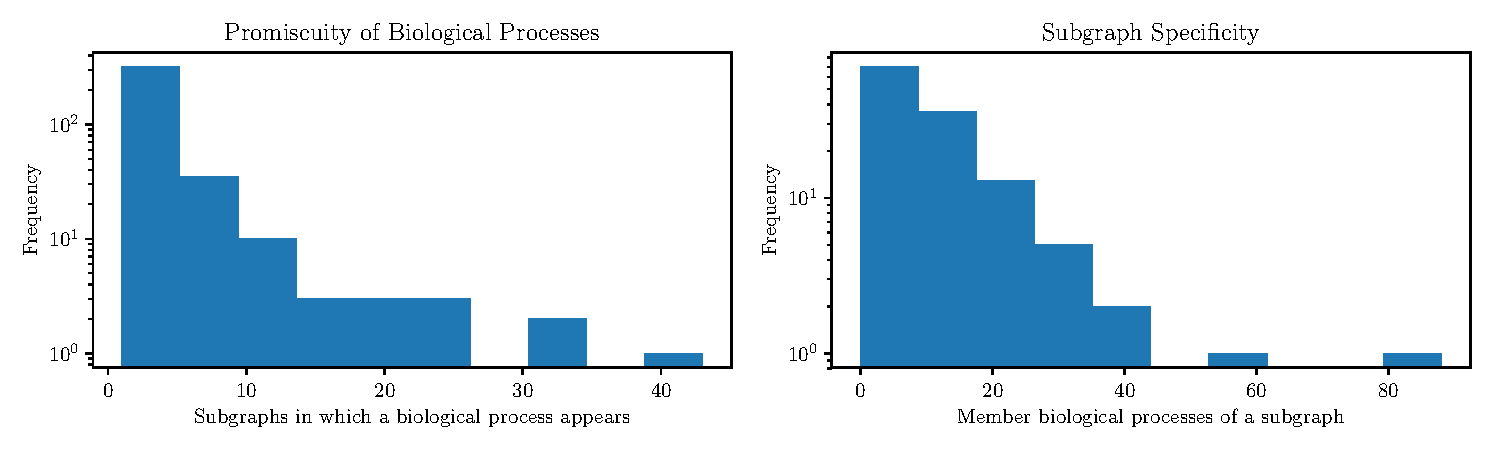
\includegraphics[width=160mm]{images/sg_comparison.pdf}}
\caption[The Landscape of Biological Process Membership in NeuroMMSig Subgraphs]{The landscape of biological process membership shows that there are both biological processes that appear in few and many subgraphs, and subgraphs with few and many biological processes.}
\label{Fig:sg_comparison}
\end{figure}

\begin{figure}
\captionsetup{format=plain}
\makebox[\textwidth]{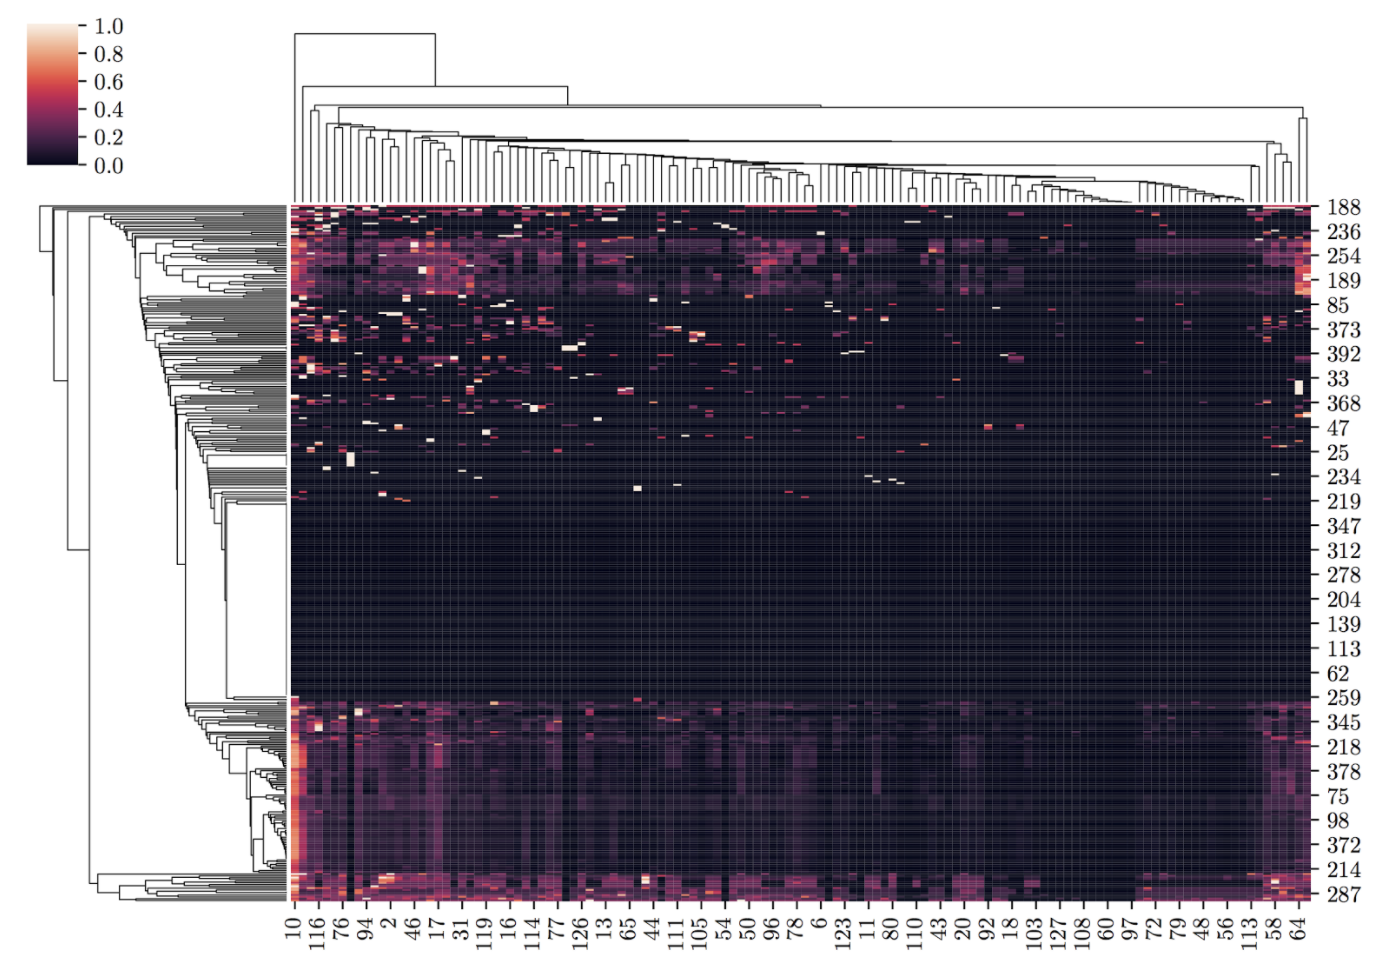
\includegraphics[width=160mm]{images/neurommsig_overlaps.png}}
\caption[Summary of the Overlap of Candidate Mechanisms with NeuroMMSig Subgraphs]{The landscape of candidate mechanism and \ac{NeuroMMSig} overlap, calculated by node overlap. The dark horizontal section directly identifies biological processes that are not annotated in any \ac{NeuroMMSig} subgraphs. This implicates their huge explanatory potential since they are outside the research dogma in Alzheimer's disease research.}
\label{Fig:neurommsig_overlaps}
\end{figure}

This landscape can also be used to annotate new candidate mechanisms to the dogmatic subgraphs in \ac{NeuroMMSig} to allow for more relevant mechanistic analysis. The annotation of further biological processes to subgraphs (Figure 17) can also allow the enrichment strategies in the \ac{NeuroMMSig} Mechanism Enrichment Server to perform enrichment over nodes corresponding to concepts on other scales.

\subsection{Candidate Mechanism Perturbation Amplitude}

All of the previous ideas from this thesis cumulate in the ability to devise and implement an algorithm for data-driven, schema-free analysis of networks. After networks are curated, parsed, enriched, checked for robustness, and triaged into unbiased candidate mechanisms, they can finally be analyzed. This section presents the candidate mechanism perturbation amplitude algorithm. It addresses the issues posed by previous algorithms with more complex randomized approaches and ultimately enables analysis of new modes of data by using a classical schema-free analytical technique similar inspired by other heat diffusion analyses in networks biology \cite{Bernabo2014,Leiserson2015}. The example presented below includes the use of differential gene expression analysis from Alzheimer's disease applied to the unbiased candidate mechanisms generated from the \ac{NeuroMMSig} knowledge assembly.

In this algorithm, heat is applied to the nodes based on the data set. For the differential gene expression experiment, the log-fold-change values were used instead of the corrected p-values to allow for the effects of up- and down-regulation to be admitted in the analysis. Finally, heat diffusion was run with the constraint that decreases edges cause the sign of the heat to be flipped. Because of the construction of unbiased candidate mechanisms, all heat will flow towards their seed biological process nodes. The amount of heat on the biological process node after heat diffusion stops becomes the score for the whole candidate mechanism.

Because heat always flows towards the biological process node, it is possible to remove leaf nodes (nodes with no incoming edges) after each step, since their heat will never change. 

The issue of inconsistent causal networks addressed by the SST algorithm does not affect heat diffusion algorithms since it can quantify multiple conflicting pathways. However, it does not address the possibility of contradictory edges, for example, when A increases B and A decreases B are both true. A random sampling approach is used on networks with contradictory edges and aggregate statistics over multiple trials are used to assess the robustness of the scores as a function of the topology of the underlying candidate mechanisms.

Finally, this algorithm can be tuned to allow the use of correlative relationships. Because many multi-scale and multi-modal data are often measured with correlations to molecular features, this enables experiments to be run using SNP or brain imaging features, whose experiments often measure their correlation with the activity of gene products. 

\subsection{Application Scenario}

This algorithm was applied with the Alzheimer's disease knowledge assembly to assist in interpretation of the differential gene expression experiments from GSE28146 \cite{Blalock2011}. This trial classified patients into three disease progression stages: early, moderate, and severe. While BEL has inherent limits in its temporal expressivity, interpreting data that has an inherent temporal ordering helps overcome this limit. The results for each time point can be accessed at \verb|https://github.com/pybel/pybel-notebooks/blob/master/results/time_series_cmpa.csv|.

\begin{figure}
\captionsetup{format=plain}
\makebox[\textwidth]{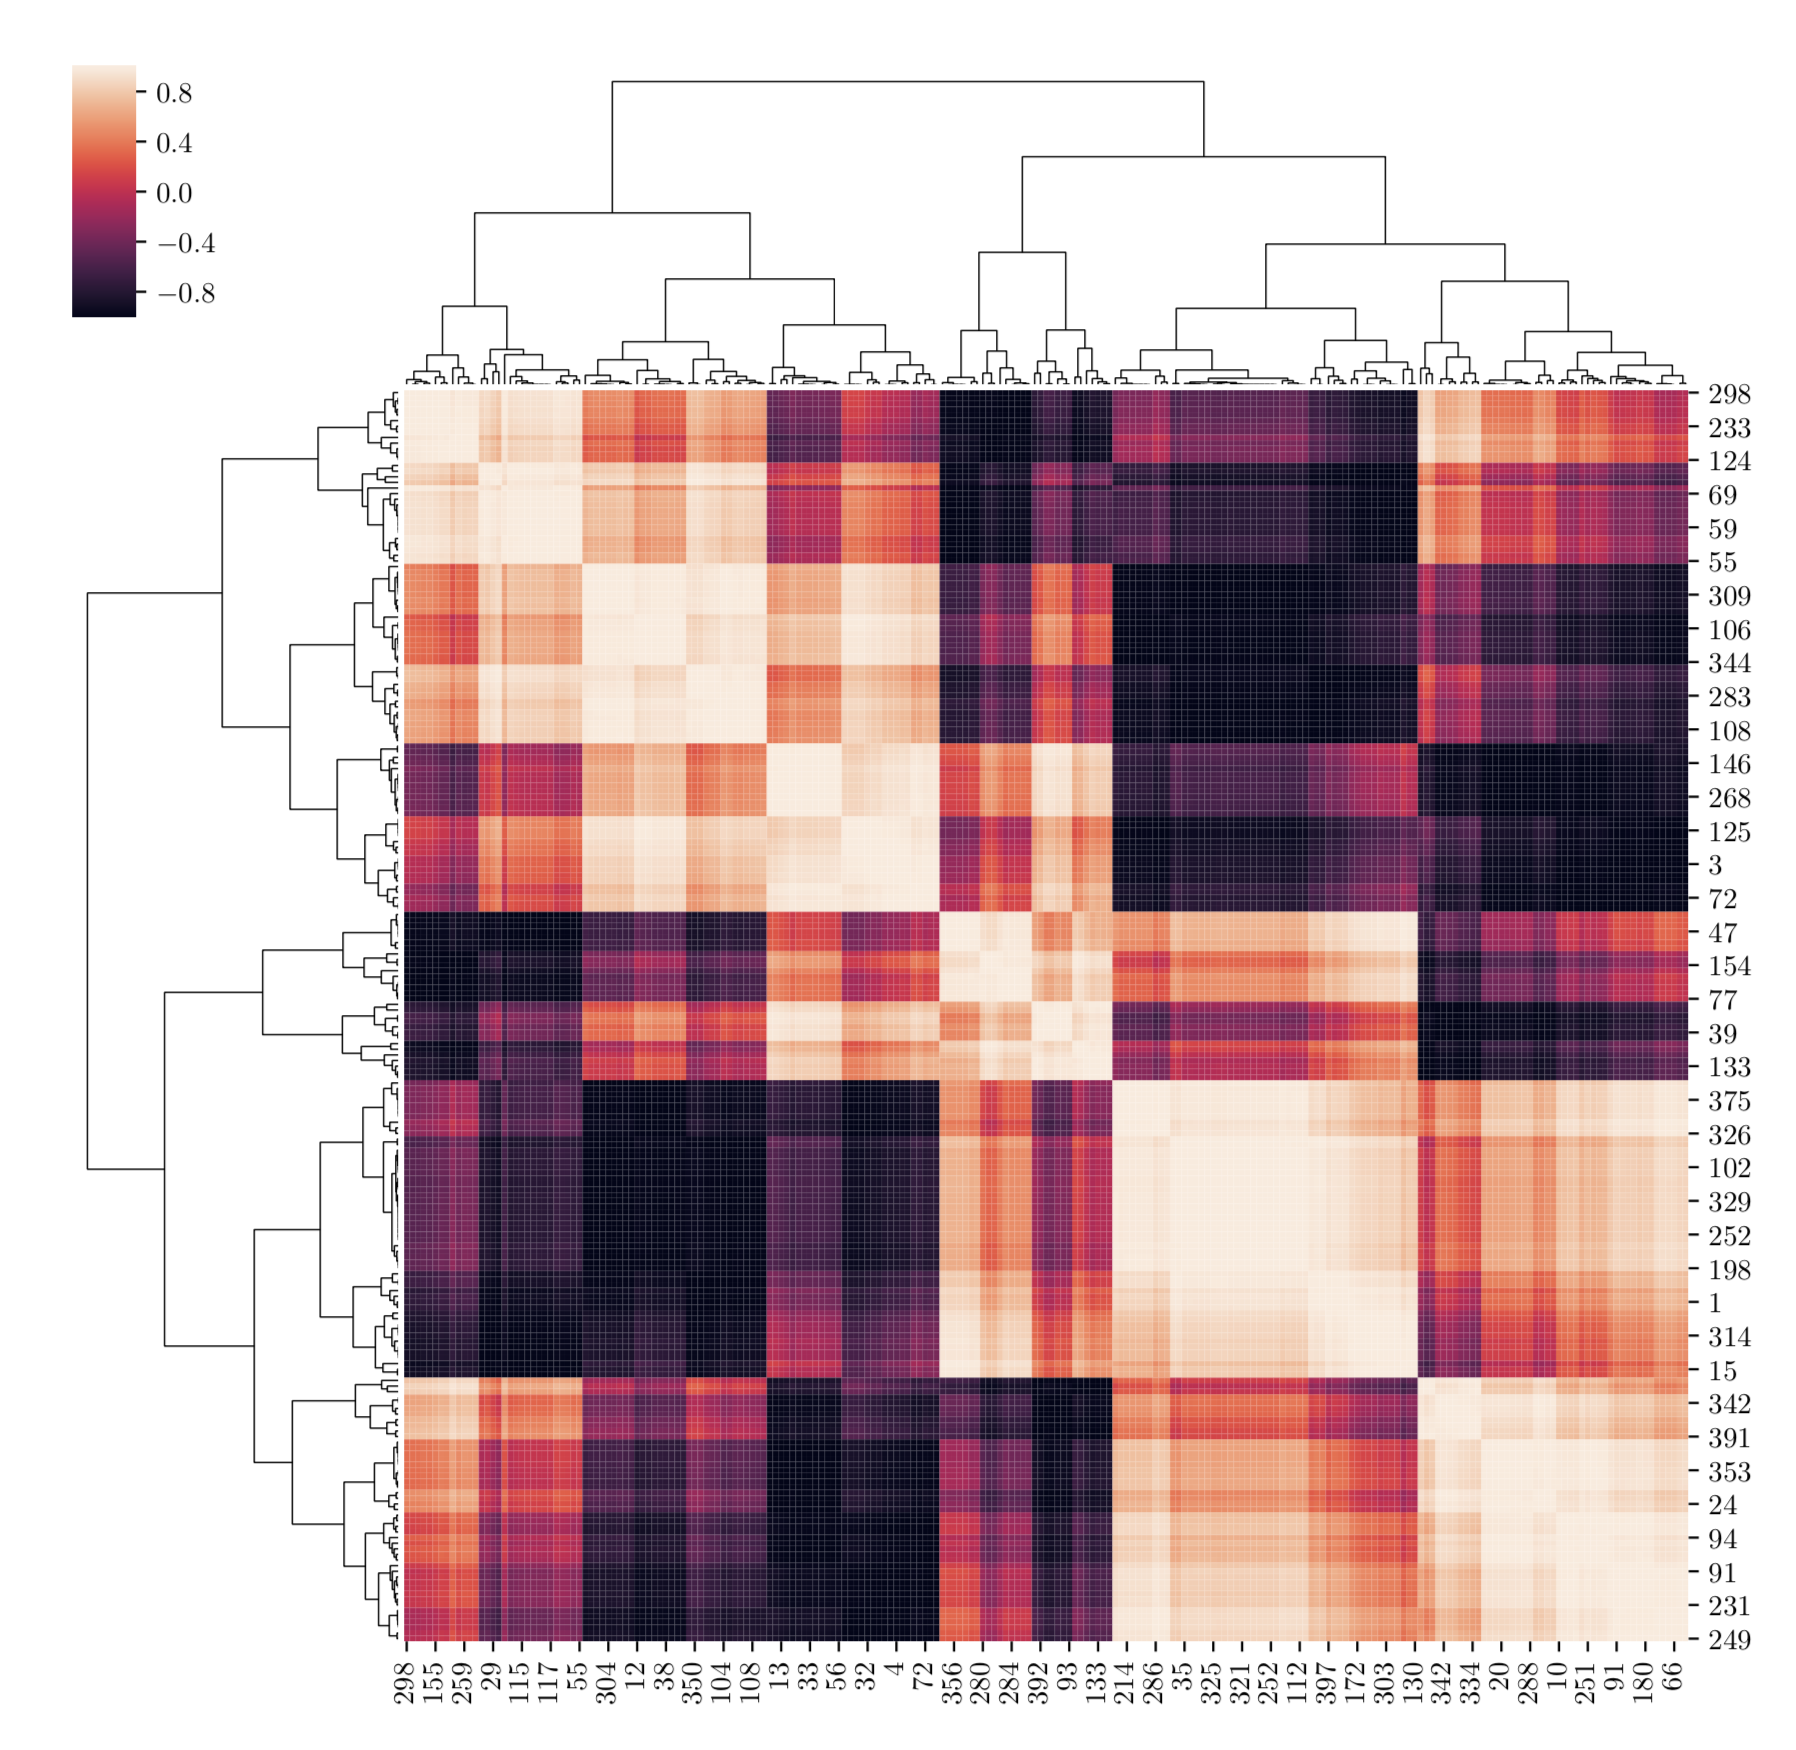
\includegraphics[width=160mm]{images/time_series_clustering.png}}
\caption[Clustering of Time-series Candidate Mechanism Perturbation Amplitude Scores]{A hierarchical clustering over the Pearson correlation of each candidate mechanism score through time suggests there are 4-6 discernible classes.}
\label{Fig:time_series_clustering}
\end{figure}

\begin{figure}
\captionsetup{format=plain}
\makebox[\textwidth]{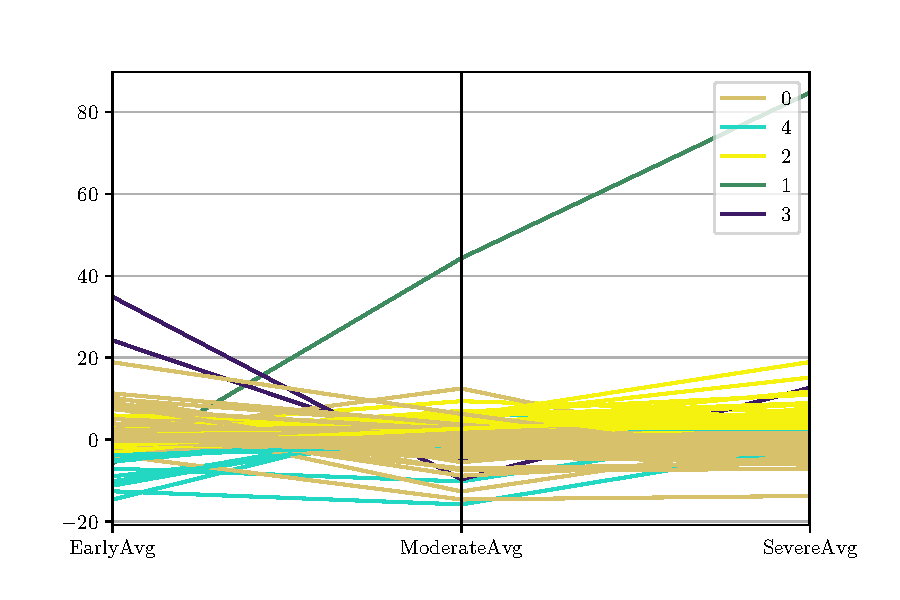
\includegraphics[width=120mm]{images/time_series_pc.pdf}}
\caption[Time-series Candidate Mechanism Perturbation Amplitude Score]{Parallel coordinate plot of all candidate mechanism with coloring by cluster shows the different progressions of biological processes.}
\label{Fig:time_series_pc}
\end{figure}

A hierarchical clustering (Figure 18) was performed using the Pearson correlation coefficient to group biological processes whose observed perturbation changed similarly through time. The dendrogram suggested there were between 4-6 groups of similarly varying processes. In order to make an interpretation, the original values are displayed in a parallel coordinate plot (Figure 19) with colors corresponding to their classes.

In figure 19, class 1 (green) is consists of biological processes that continually increase throughout the progression of the disease. Notably, it contains the inflammatory response. Class 3 (purple) contains biological processes that decrease from the early to moderate stage then increase again. This refers to cell death and neuron death processes. Class 4 includes processes that are initially down-regulated then become less regulated, including mitochondrion-related pathways. Class 2 (yellow) includes processes that do not become disregulated until the severe onset of disease, and have much more variety from glutamate secretion to ion homeostatic processes to metabolic processes. The remaining class does not show significant regulation in any of the disease stages. 

While Alzheimer's disease must be studied with respect to its progression over time, this analysis can provide insight directly to measurements performed on a single time series. Those results provide a ranking that prioritizes the most up- and down-regulated biological processes as a function of the observed data. 


\chapter{Conclusion and outlook}

This master's thesis was originally motivated by the desire to automatically interpret data sets and generate hypotheses using prior knowledge. While working towards that goal, it was necessary to develop an entire computational infrastructure for BEL. That infrastructure was extended with reusable components to integrate prior knowledge from other sources in order to model biology at the finest granularity possible. Next, a framework for testing the validity and robustness of those knowledge assemblies was implemented and applied to the \ac{NeuroMMSig} knowledge base. Finally, algorithms for extracting meaningful subnetworks were applied to enable schema-free and multi-modal analysis using a heat diffusion algorithm. Using this workflow, it is now possible to interpret multi-modal data sets and generate hypotheses in a truly automated fashion.


\printbibliography
	
\backmatter

\chapter*{Declaration}
I hereby certify that this material is my own work, that I used only those sources and resources referred to in the thesis, and that I have identified citations as such.
		
\vspace{0.3in}

\noindent Bonn, \today

\vspace{1in}

\noindent Charles Tapley Hoyt

\end{document}
